\chapter{\uppercase{$^{227}$Ac as a Calibration Source}} \label{ch:Ac}

\section{Motivation}

In the absence of an eV-scale sterile neutrino PROSPECT should measure IBD rates that fall like one over distance from the reactor squared. 
If sterile neutrino oscillation was detected, after one year PROSPECT would measure the spectrum seen in Figure~\ref{fig:lovere1yr}, given a mass splitting of 1.78 eV$^2$, .
However, a situation could occur in which a sterile neutrino did not exist, or could not be measured with PROSPECT, and an oscillation is still measured.
This could happen if there are segment to segment volume variations throughout the detector, mimicking an oscillation signal.
Therefore, it becomes important that the product of efficiency$\times$volume for all segments is well known. 

\begin{figure}[h]
	\centering
	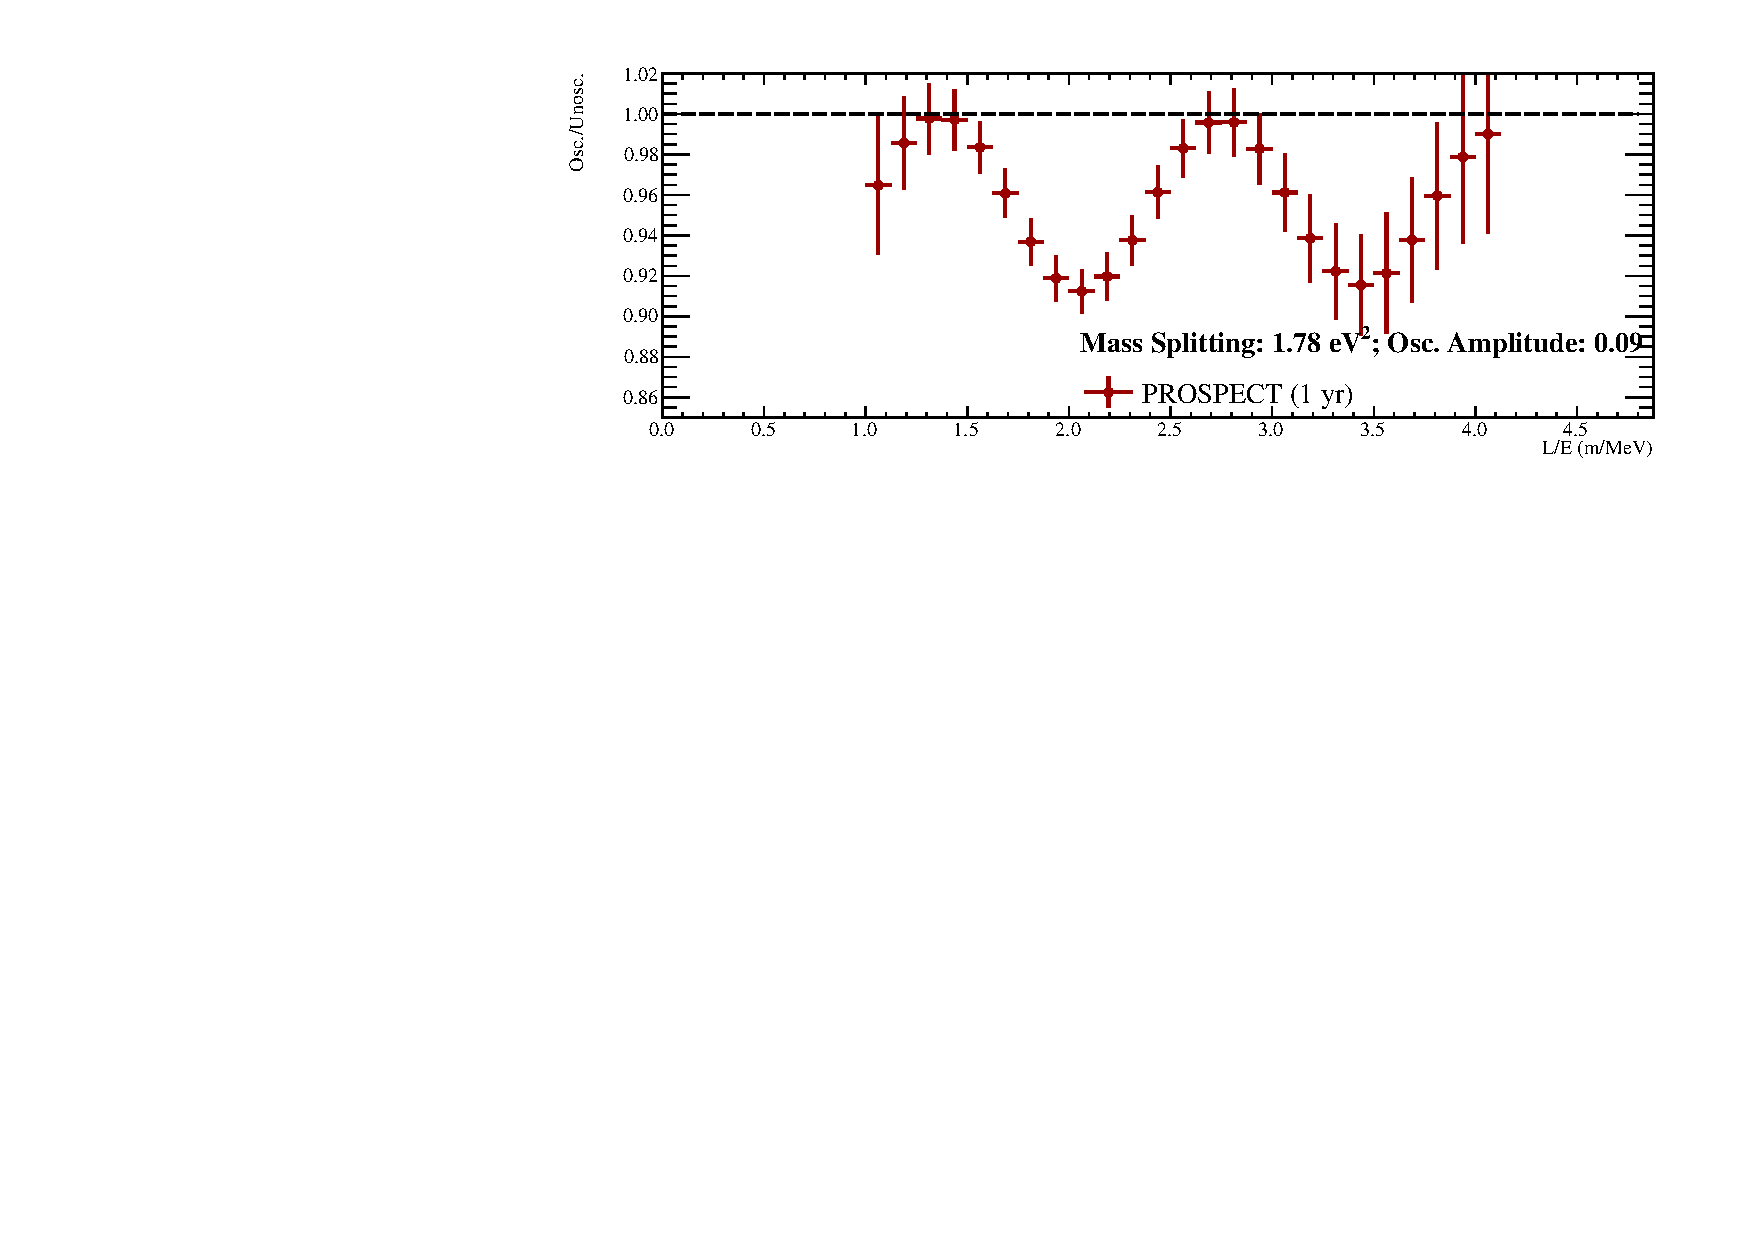
\includegraphics[width=0.7\linewidth]{tex/6-ac227-images/LoverE_1yr}
	\caption[Monte Carlo neutrino spectrum as a function of L/E]{The ratio of the oscillated to un-oscillated neutrino spectrum as a function of L/E that would be observed by PROSPECT after 1 year if a sterile neutrino signal was detected \cite{PSurukuchi:1534}.}
	\label{fig:lovere1yr}
\end{figure}


This measurement can be accomplished if an event source is uniformly distributed throughout the active volume of the detector. 
By measuring the rate of this source in each segment the relative volumes can be compared and tracked through time.
\Ac was chosen as the source and a chloride solution was prepared and dissolved in the liquid scintillator to ensure uniform distribution.

\Ac was chosen for several reasons. First, because an \AaAa coincidence occurs in its decay chain, specifically $^{219}$Rn $\rightarrow ^{215}$Po + $\alpha \rightarrow ^{211}$Pb + \Aa, as highlighted in Figure~\ref{fig:ac227chain}.
\Rn has a half-life of 3.96 $\pm$ 0.01 s and $\alpha$-decays 100\% of the time, while \Po has a half-life of 1.781 $\pm$ 0.005 ms and $\alpha$-decays  99.99977(2)\% of the time \cite{ENSDF}, so the \AaAa coincidences happen frequently.
The \Aa decay of \Po is mono-energetic at 7.39 MeV which results in a $\sim$0.78 MeVee signal after quenching, well removed from nLi captures that occur around 0.5 MeVee. 
In addition, there are no corresponding gammas with the \Po decay, making this a very clean and well defined signal.
The \Rn \Aa decays are not so nice, as there are four dominant alpha energies and three dominant gamma energies for these decays, as listed in Table~\ref{tab:RnPoE}, but the use of time, energy, and PSD cuts make them easy to pair with corresponding \Po decays.

\begin{figure}[hb]
	\centering
	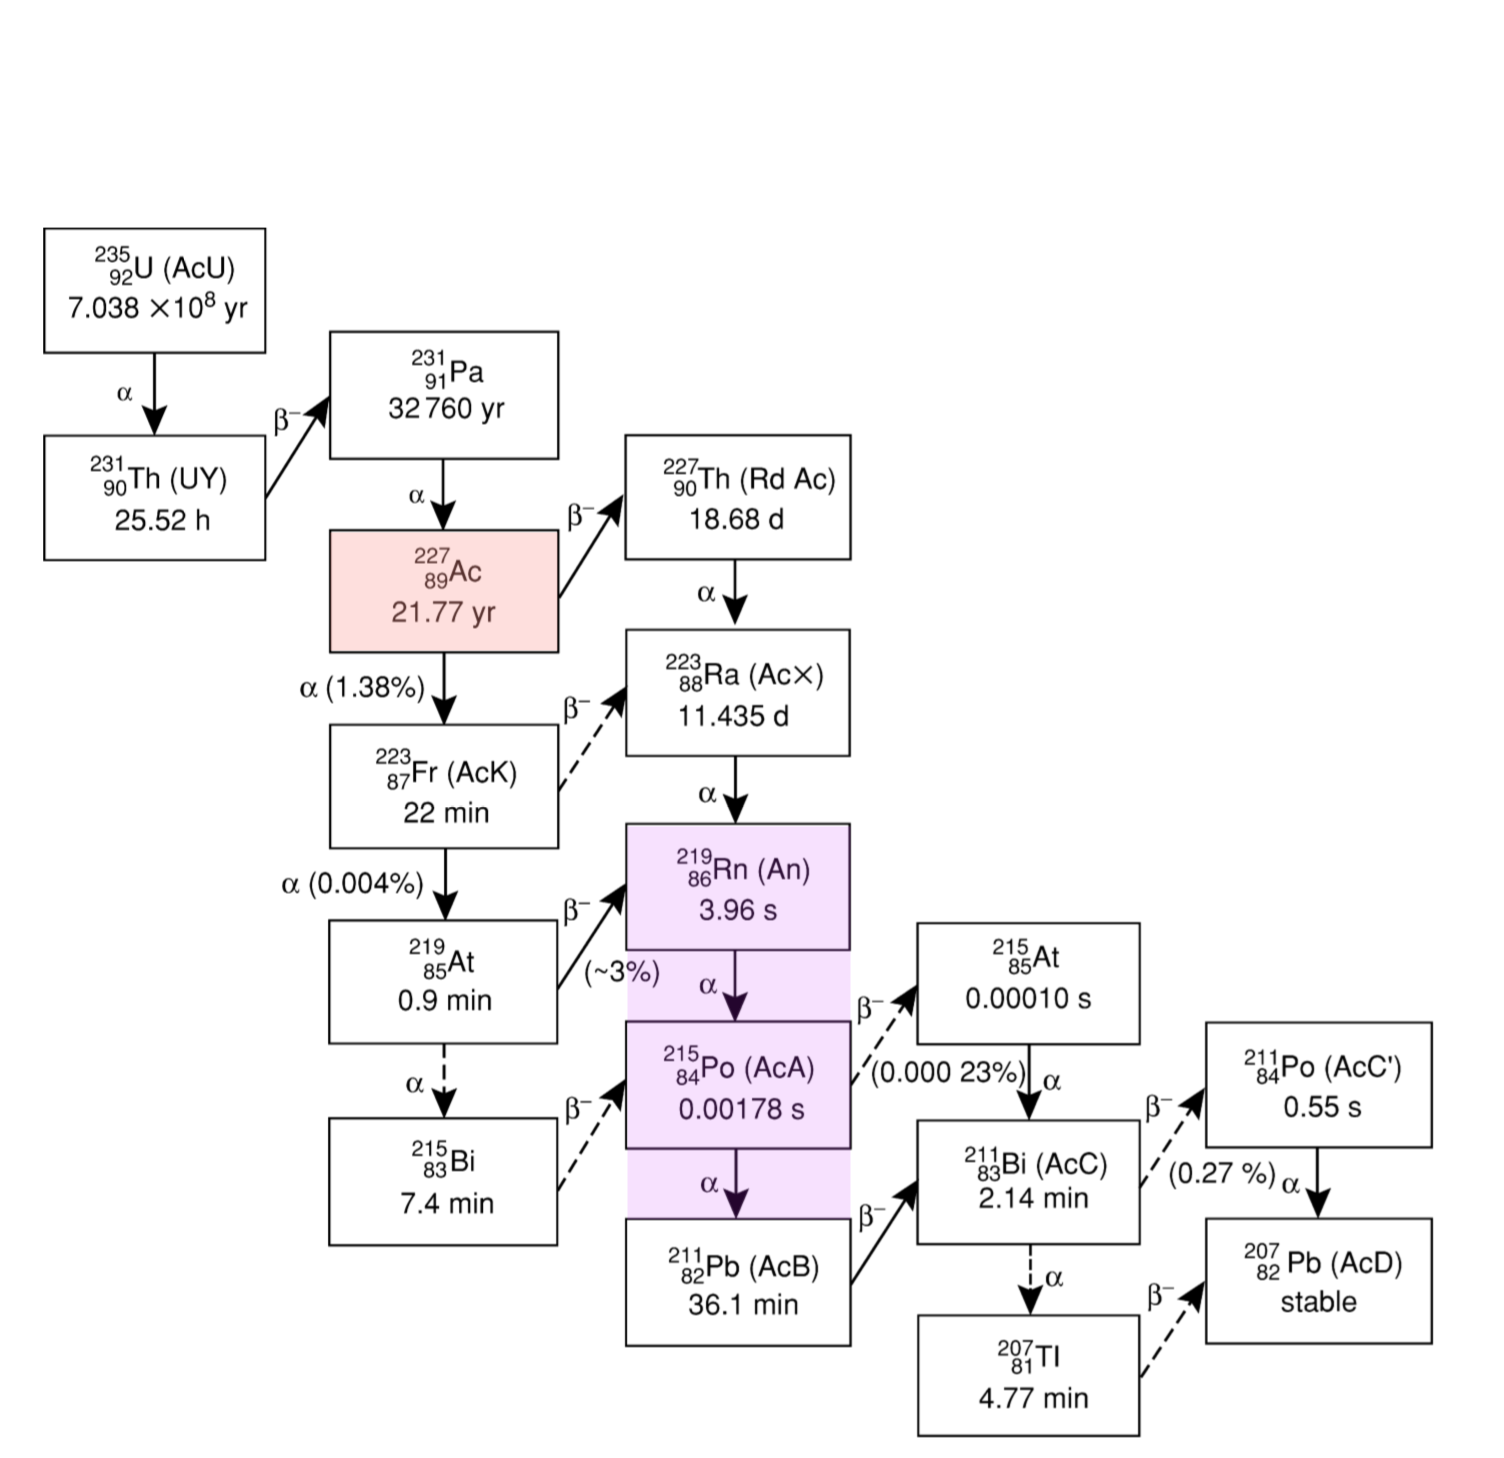
\includegraphics[width=0.6\linewidth]{tex/6-ac227-images/Ac227Chain}
	\caption[\Ac decay chain]{The full decay chain of \Ac (a daughter of $^{235}$U), in which the \AaAa coincidence of interest is highlighted \cite{Kirby2011}.}
	\label{fig:ac227chain}
\end{figure}

\begin{table}[h]
	\centering
\begin{tabular}{|c|c|c|c|c|c|}
	\hline 
	& E$_\alpha$ [keV] & I$_\alpha$ \% &  & E$_\gamma$ [keV] & I$_\gamma$ \% \\ 
	\hline 
	\Rn & 6425.0(10) & 7.5(6) &  & 271.23(1) & 10.8(6) \\ 
	%\hline 
	& 6530(2) & 0.110(10) &  & 401.81(1) & 6.6(4) \\ 
	%\hline 
	& 6552.6(10) & 12.9(6) &  & 130.60(3) & 0.13(9) \\ 
	%\hline 
	& 6819.1(3) & 79.4(10) &  &  &  \\ 
	\hline 
	\Po & 7386.1(8) & 99.999770(20) &  &  &  \\ 
	\hline 
\end{tabular} 
\caption[$\alpha$ and $\gamma$ energies of \Rn and \Po decays]{Energy and absolute intensity of dominant $\alpha$ and $\gamma$ decay radiation for \Rn and \Po. Decay energies not listed here have an intensity of $< $0.05\%.}
\label{tab:RnPoE}
\end{table}

%\begin{figure}[h]
%	\centering
%	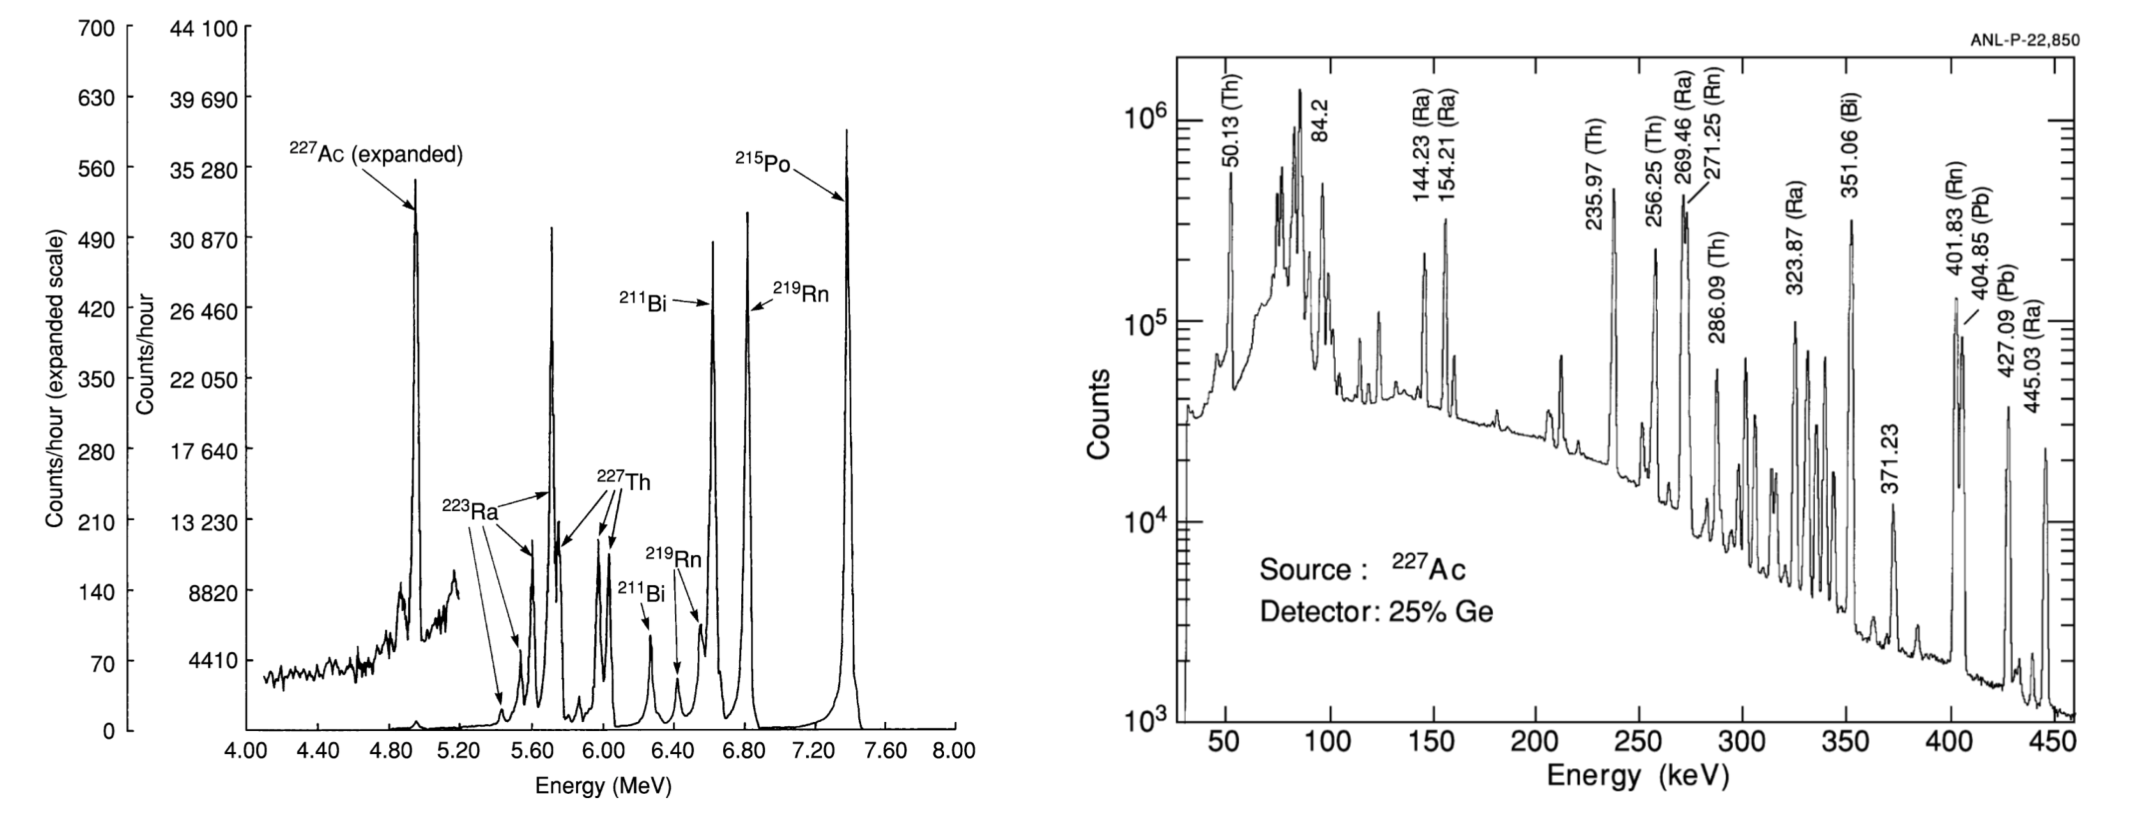
\includegraphics[width=0.95\linewidth]{tex/6-ac227-images/Actinium_agSpectrum}
%	\caption[]{\cite{Kirby2011}}
%	\label{fig:actiniumagspectrum}
%\end{figure}


\section{Material Compatibility}

Before \Ac could be added to the PROSPECT detector, it had to be determined that \Ac and its daughters would not adsorb onto detector materials.
If it was adsorbed then it would not be a uniform source in the detector, nullifying its use as a method to track relative efficiency$\times$volume throughout the detector.
To test this six material samples were placed in vials of $^6$Li-LS spiked with \Ac. The rate of \Ac in each sample vial and one reference vial with no material was measured and tracked over a period of 6 months. 
An observation of a significant decrease in rate, relative to the half-life of \Ac, would indicate that \Ac was adsorbing onto the material.

\subsection{Material and Scintillator Preparation}
The materials tested were: ultraviolet transmitting (UVT) acrylic, flourinated ethylene propylene (FEP), polylactide (PLA), polyether ether ketone (PEEK), a RG 188 cable, and viton o-rings. See Table~\ref{tab:materials} for a list of their uses in the detector and sample sizes.
To prepare the materials they were all placed in a single beaker with ultra-pure water and cleaned ultrasonically for 30 minutes.
They were then transferred to a watch glass and placed in a 50 C over for two hours.
After drying they were placed in empty 12 mL vials.

The \Ac used to spike the scintillator was obtained from Eckert and Ziegler as a solution of 3.711$\times$10$^4$ Bq $\pm$ 1.32\% of \Ac in 10.22710 g of 1 M HCl, measured on September 6, 2016.
0.503 g of this solution was added to 192 g of $^6$Li-LS on December 15, 2016.
With a half-life of 21.772 $\pm$ 0.003 yrs \cite{ENSDF}, the activity of the \Ac solution before adding to the LiLS was 36788 Bq, yielding a final activity of 94.2 Bq/10 g. 
This is the stock solution from which all LS was taken for the material studies and later on for spiking the detector.

\begin{table}[H]
	\centering
\begin{tabular}{|p{0.17\textwidth}|p{0.45\textwidth}|p{0.33\textwidth}|}
	\hline 
	\textbf{Material} & \textbf{Detector Use} & \textbf{Sample Size} \\ 
	\hline 
	UVT Acrylic & Front window of PMT housing & 1.0 $\times$ 1.15 $\times$ 0.1 cm$^3$ \\ 
	\hline 
	FEP  & Film on optical separators & 1.5 $\times$ 1.5 cm$^2$, 3 mm thick \\ 
	\hline 
	PLA & 3D printed pinwheels & 10 disks; 0.5 cm diameter, 0.1 cm thick \\ 
	\hline 
	PEEK & Seal plugs through which the high voltage and signal cables were threaded. Screws used to bolt together segment supports. Spacers at the base of the acrylic tank. & 1 Nut; ID 0.5 cm, small OD 1cm, large OD 1.1cm, thickness 0.5 cm \\ 
	\hline 
	RG188 Cable & High voltage and signal cables & 4.5'' long \\ 
	\hline 
	Viton O-ring & Seal back plugs of PMT housings and seal acrylic tank & 10 O-rings; OD 6mm, ID ~3mm, thickness 1.5mm \\ 
	\hline 
\end{tabular} 
\caption{Samples used to test if \Ac or its daughters would adsorb onto detector materials.}
\label{tab:materials}
\end{table}

\begin{table}[H]
	\centering
\begin{tabular}{|c|c|c|}
	\hline 
	\textbf{Material} & \textbf{Date Filled} & \textbf{Weight of LiLS Added (g)}  \\ 
	\hline 
	Reference & 12/15/2016 & 10.030 \\ 
	\hline 
	UVT Acrylic & \multirow{6}{*}{02/24/2017}  & 9.98 \\ 
	%\hline 
	FEP &  & 9.98 \\ 
	%\hline 
	PLA &  & 9.999 \\ 
	%\hline 
	PEEK &  & 9.99 \\ 
	%\hline 
	RG188 Cable &  & 9.981  \\ 
	%\hline 
	Viton O-ring &  & 10.011  \\ 
	\hline 
\end{tabular} 
\caption{The weight of \Ac spiked LiLS that was added to each sample vial.}
\label{tab:MatFill}
\end{table}

Prior to filling all sample vials the threads of each vial were wrapped with teflon tape in an effort to obtain a secure seal. 
The reference vial was filled on December 15, 2016 with 10.030 g of \Ac spiked LiLS from the stock solution, yielding an expected activity of 94.5 Bq.
All material vials were filled on February 24, 2017 with the amount of stock solution added to each listed in Table~\ref{tab:MatFill}.
At the time of filling the rate in each vial was expected to be $\sim$93 Bq.
For a photograph of all filled material sample vials see Figure~\ref{fig:samples}.

\begin{figure}[h]
	\centering
	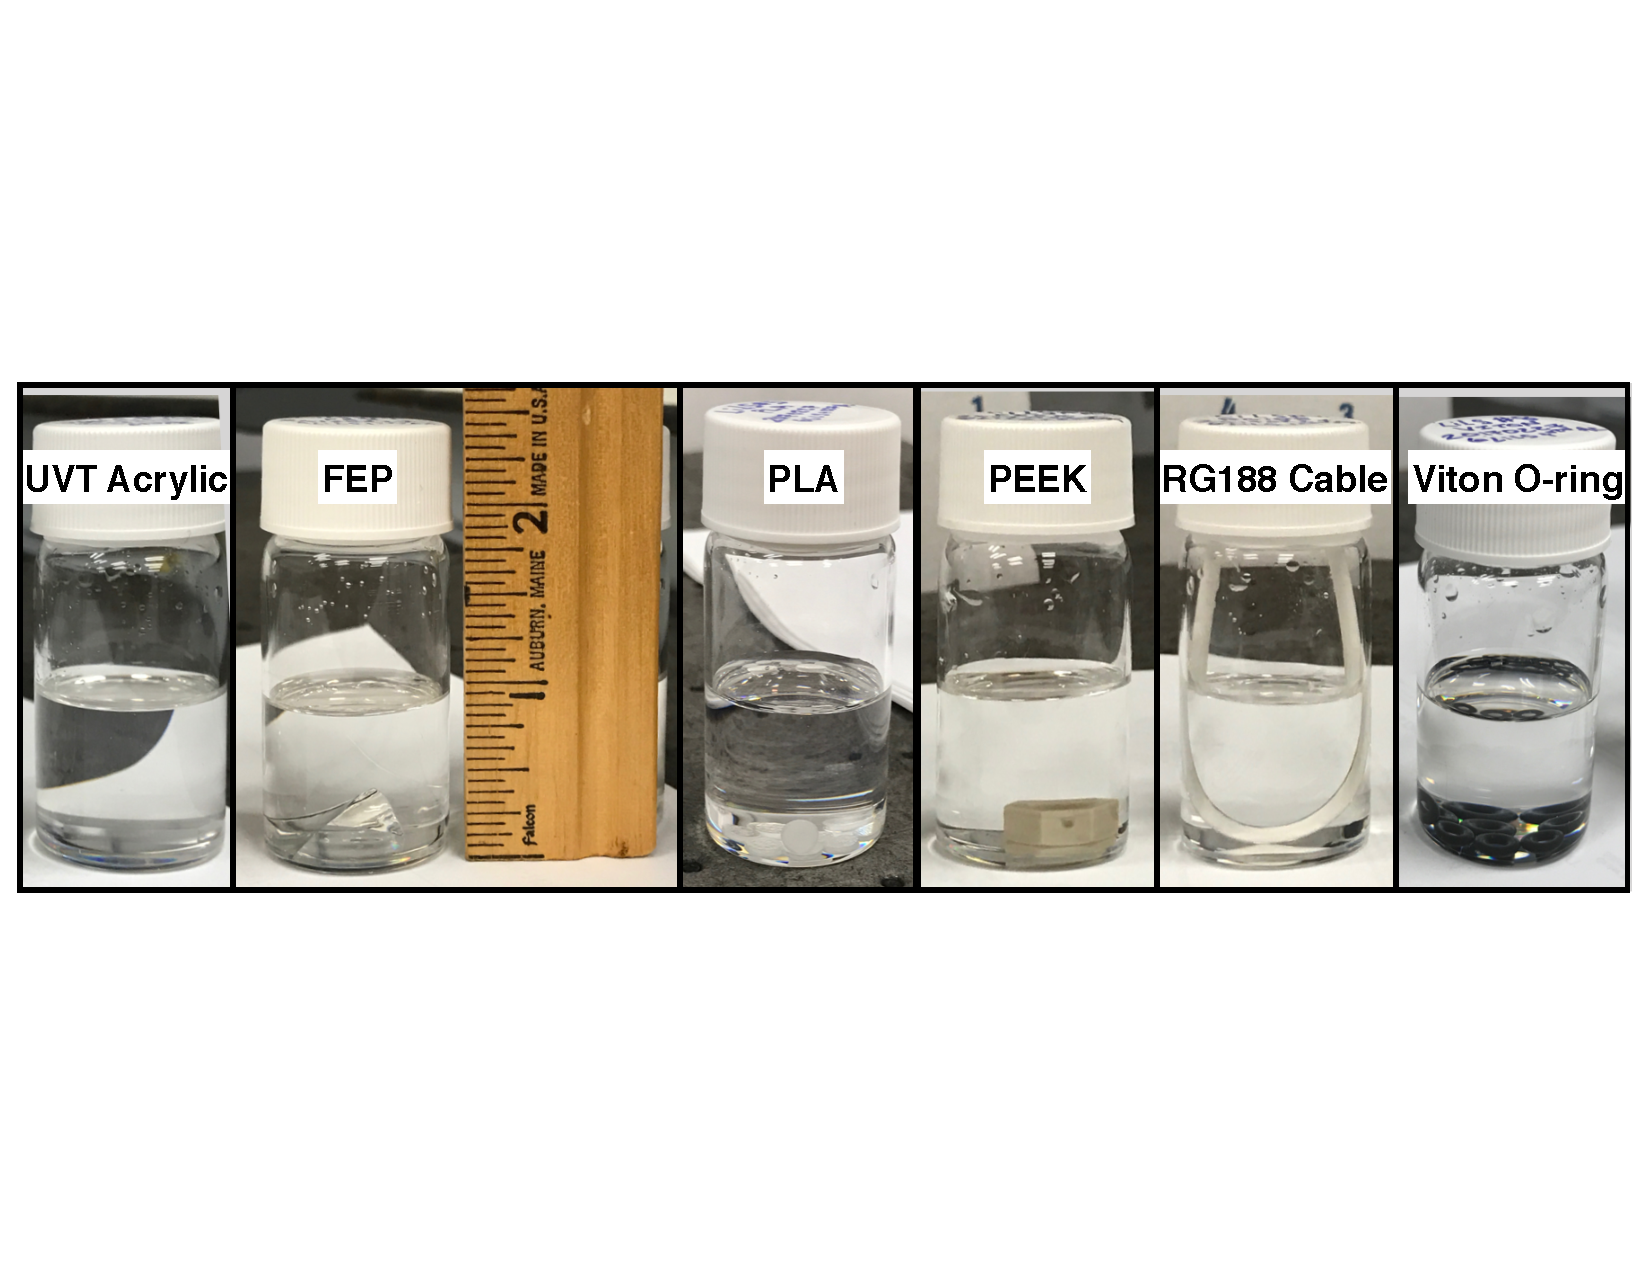
\includegraphics[width=0.8\linewidth]{tex/6-ac227-images/BNL/Samples}
	\caption[Material sample vials]{Photos of all material sample vials filled with \Ac spiked LiLS, with ruler for scale.}	
	\label{fig:samples}
\end{figure}

\subsection{Detector}

The detector consisted of a 2'' photomultiplier tube coupled using optical grease to a solid cylinder of UVT acrylic painted white with an insert cut out to hold the sample vials, as shown in Figure~\ref{fig:blackbox}.
Placed in a dark box the PMT is cabled to a CAEN DT55xx Desktop HV Power Supply and a CAEN DT5730 8 Channel 14-bit 500 MS/s Digitizer \cite{CAENDigit}.
A modified version of Wavedump 3.7.2 \cite{CAENWD} was used to start and stop the data runs and save the waveforms of the signals.

\begin{figure}[H]
	\centering
	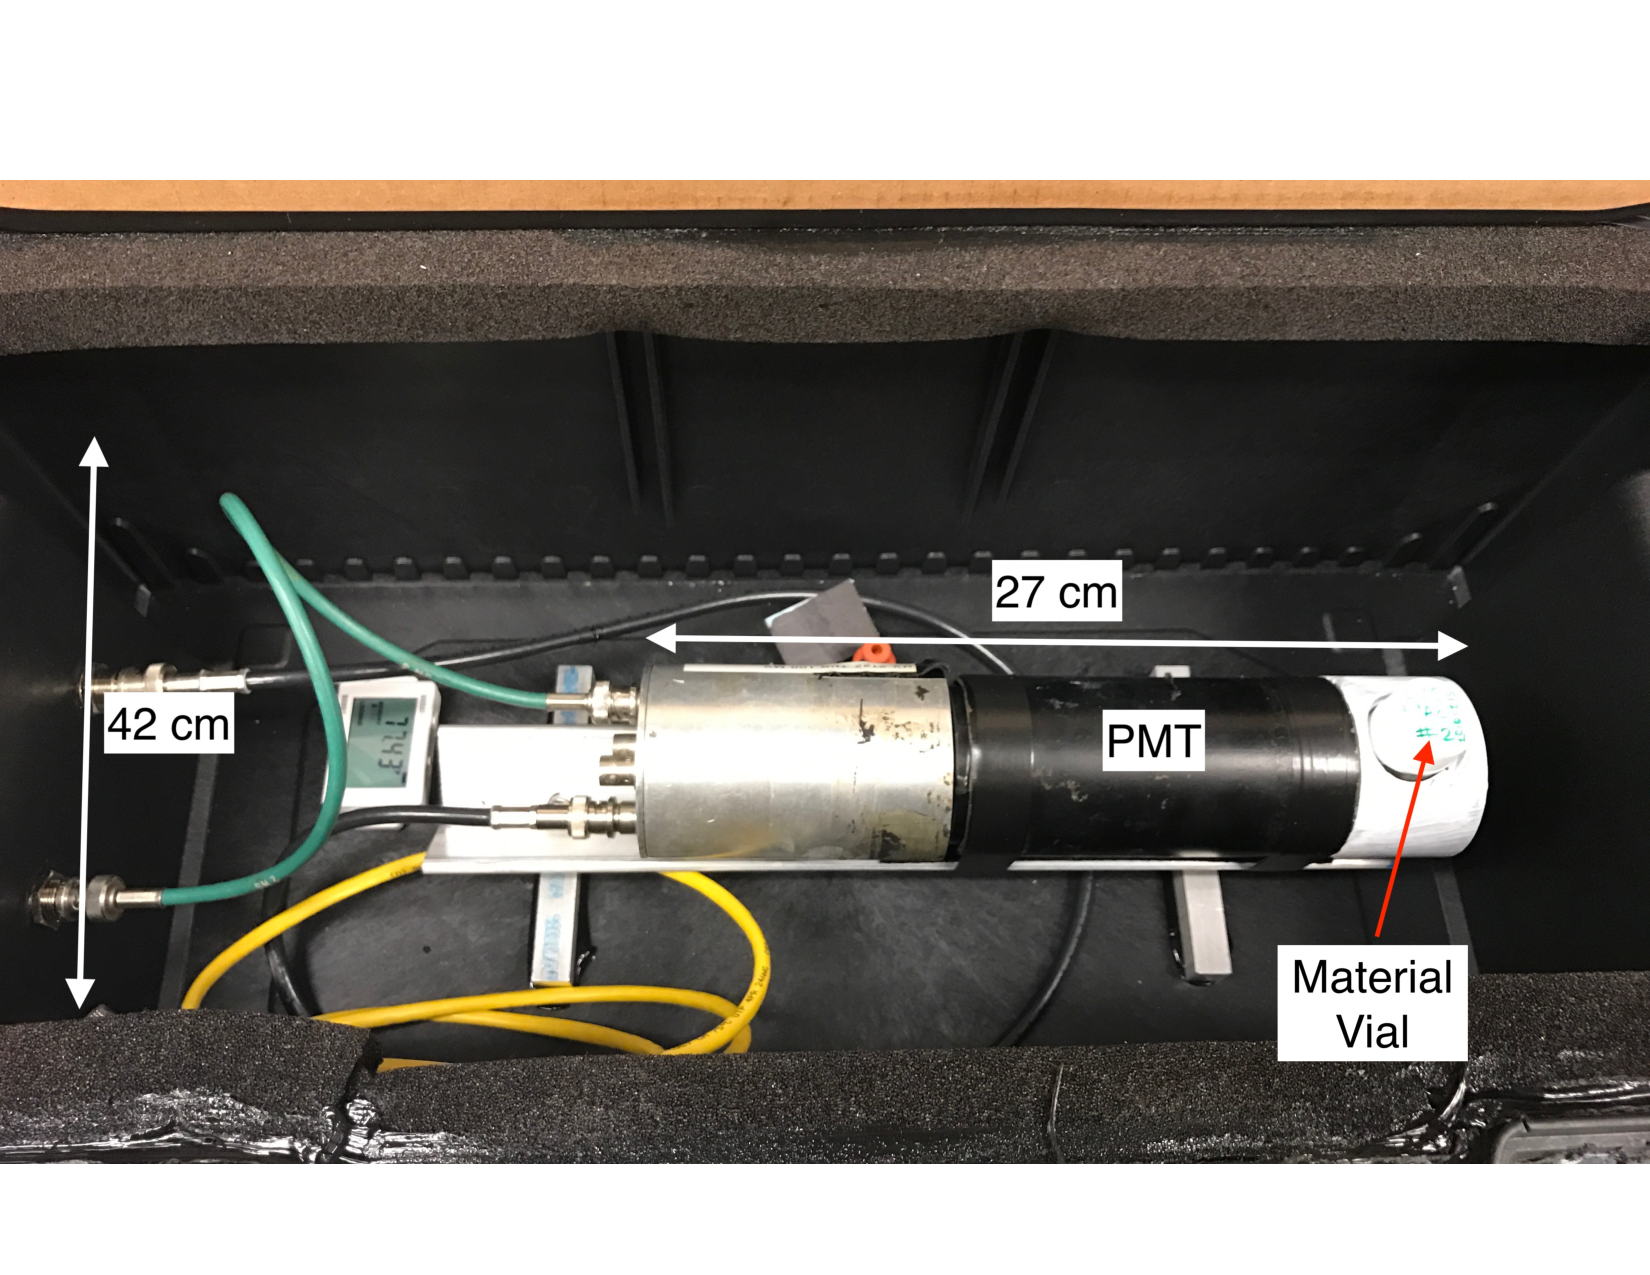
\includegraphics[width=0.7\linewidth]{tex/6-ac227-images/BNL/BlackBox}
	\caption[Detector used for material adsorption studies]{Detector used for material studies, consisting of a 2'' PMT coupled to an acrylic cylinder holding the sample vials, all contained in a dark box. The PMT is cabled to a power supply and digitizer that exist outside of the box.}
	\label{fig:blackbox}
\end{figure}

\subsection{Data Analysis}

The raw waveforms are analyzed to calculate the energy and PSD of each signal. 
Each collected waveform consists of 250 2 ns samples.
The energy is measured by taking the integral of the waveform using the trapezoidal rule in ADC units.
The total energy is converted to nC using
\begin{equation}
E[nC] = E[ADC] \times \frac{1\times10^9}{R\times\textrm{sample-rate}\times n[ADC/V]}
\end{equation}
where $R$, the resistance, is 50 $\Omega$, the sample-rate is $5\times10^8$ Hz, and $n = (2^{14} -1)/2 = 8191.50$ ADC/V.
The tail and total fractions used to calculate the PSD are both measured from the leading half-maximum point.
The total is measured as the integral from 10 samples before the half-max to 140 samples after.
The tail is measured as the integral from 19 samples after the half-max to 140 samples after.

The \Ac coincident alpha events, labeled RnPo events for the remainder of this document, are found by applying a set of timing, energy, and PSD cuts along with an accidental background subtraction.
Po events are found first by applying the energy and PSD cuts listed in Tabel~\ref{tab:MatCuts}. 
Rn coincidental events are found by looking in a 12.85 ms time window before a given Po event and applying the same energy and PSD cuts.
This time window is 5 times the lifetime of Po, 2.57 ms, allowing the collection of all possible coincident events.
Accidental events are found by looking in the same length time window, using the same energy and PSD cuts, but offset 10 Po lifetimes before a given Po event.
RnPo events are then found by subtracting the accidental events from the coincident events.
See Figure~\ref{fig:rnpoenpsd} for an example of typical energy and PSD distributions.

\begin{table}[H]
	\centering
	\begin{tabular}{c|c}
		\hline 
		Energy & 0.01 $<$ E $<$ 0.055 nC \\ 
		\hline 
		PSD & 0.31 $<$ PSD $<$ 1.0  \\ 
		\hline 
		$\Delta$t = t$_{\mathrm{delay}}$ - t$_{\mathrm{prompt}}$ & $\Delta$t $<$ 5$\tau_{\textrm{Po}}$ \\ 
		\hline 
	\end{tabular} 
	\caption{Energy, PSD, and time cuts used to find RnPo events where $\tau_{\textrm{Po}}$ = 2.57 ms. Energy and PSD cuts are applied to both prompt and delay events.}
	\label{tab:MatCuts}
\end{table}

\begin{figure}[H]
	\centering
	\begin{subfigure}{0.5\linewidth}
		\centering
		\includegraphics[width=1.\linewidth]{"tex/6-ac227-images/BNL/RnPoEn_TimeBin23_S2"}
		\caption{}
	\end{subfigure}%
	\begin{subfigure}{0.5\linewidth}
		\centering
		\includegraphics[width=1.\linewidth]{"tex/6-ac227-images/BNL/RnPoPSD_TimeBin23_S2"}
		\caption{}
	\end{subfigure}
	\caption[Typical RnPo energy and PSD distributions]{Typical energy (a) and PSD (b) distributions for RnPo events in the reference sample after accidental background subtraction.}
	\label{fig:rnpoenpsd}
\end{figure}

The rate of RnPo events is measured by fitting the RnPo $\Delta$t distribution with
\begin{equation}
	f(t) = N_0e^{-t/\tau}
	\label{eq:MatDtFit}
\end{equation}
where $N_0$ and $\tau$, the lifetime of \Po, are allowed to vary. 
Using the fit results, the rate is then defined as
\begin{equation}
	R = \frac{N_0 \tau}{\textrm{bin-width}\times\textrm{livetime}}
\end{equation}
\begin{equation}
	\sigma_R = R \times \sqrt{  \left(\frac{\sigma_{N_0}}{N_0}\right)^2 + \left(\frac{\sigma_{\tau}}{\tau}\right)^2 + \frac{2\sigma_{N_{0}\tau}}{N_0\tau} }
\end{equation}
where the livetime is measured, for each run, as the time from the beginning of the run to the last Po event. 
An example of a typical RnPo $\Delta$t distribution can be seen in Figure~\ref{fig:rnpodttimebin23s2}. It should be noted here that the energy and PSD cuts were made wide enough so that no efficiency correction needed to be applied.

\begin{figure}[H]
	\centering
	\includegraphics[width=1.\linewidth]{"tex/6-ac227-images/BNL/RnPoDt_TimeBin23_S2"}
	\caption[Typical RnPo $\Delta$t distribution]{A typical example of the RnPo $\Delta$t distributions for the reference sample. Left: coincidental and accidental distributions found using the defined energy and PSD cuts. Right: the $\Delta$t distribution after subtraction of the accidental distribution, fit with Equation~\ref{eq:MatDtFit}.}
	\label{fig:rnpodttimebin23s2}
\end{figure}

\subsection{Results}

The RnPo rate was calculated for each material sample and the reference sample over a period of about six months. These results can be seen in Figure~\ref{fig:ratevstimeallsamples}.
Though statistical errors vary from around 0.6-1\%, overall rates vary at a rate of around 12\%, indicating systematic variations.

\begin{figure}[ht]
	\centering
	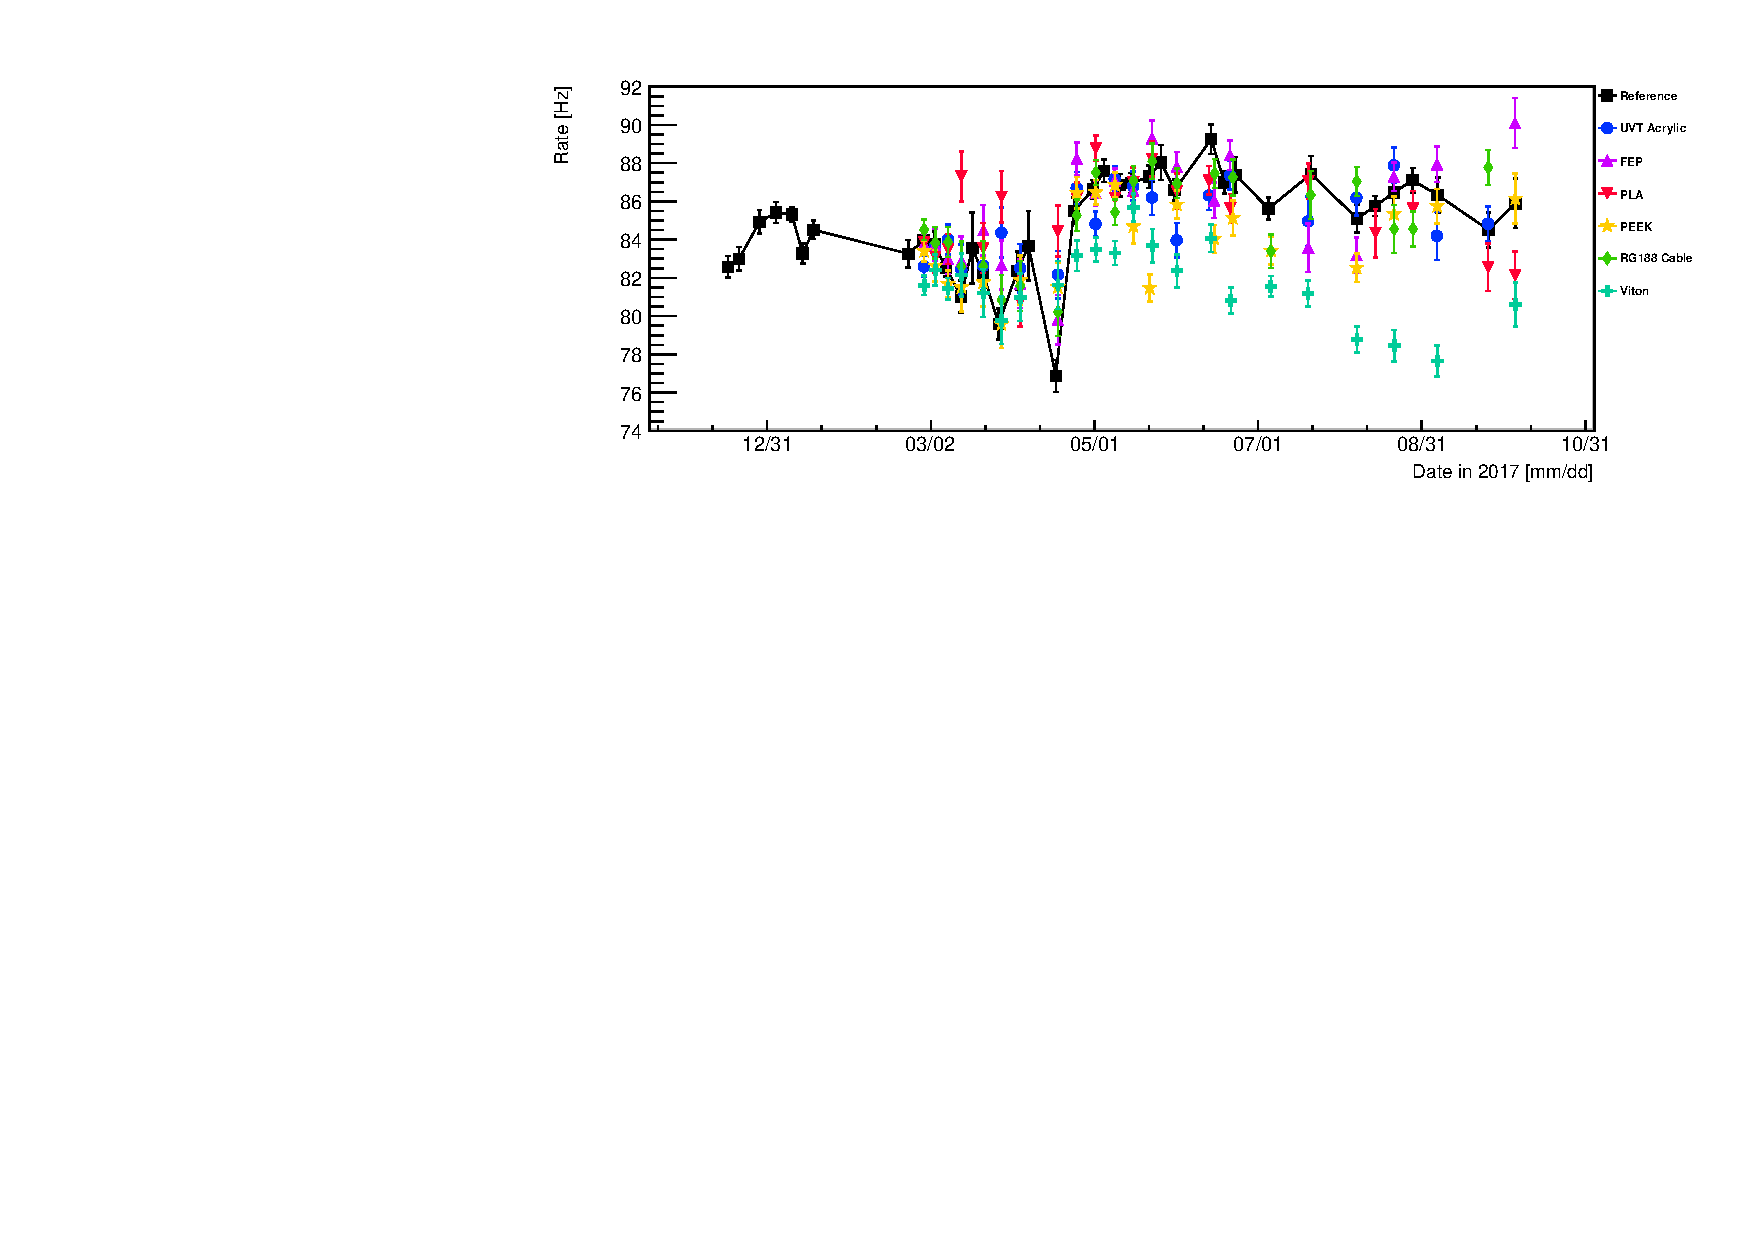
\includegraphics[width=1\linewidth]{tex/6-ac227-images/BNL/RateVsTime_AllSamples}
	\caption[\Ac rate for each material sample]{\Ac rate for each material sample. Errors are statistical.}
	\label{fig:ratevstimeallsamples}
\end{figure}

Systematic variations can be better understood by looking at the behavior of the \Po energy distribution through time.
This was done by fitting this distribution for the reference sample with a sum of two Gaussians to account for the non-Gaussian nature of the peak as demonstrated in Figure~\ref{fig:poenfittimebin23s2}.
The mean and 1$\sigma$ width of each of these Gaussians versus time is show in Figures~\ref{fig:poenmeanvstimes2} and ~\ref{fig:poenwidthvstimes2}.
It can be seen that the \Po energy mean varies about 5\% and the width around 15\%.

\begin{figure}[!b]
	\centering
	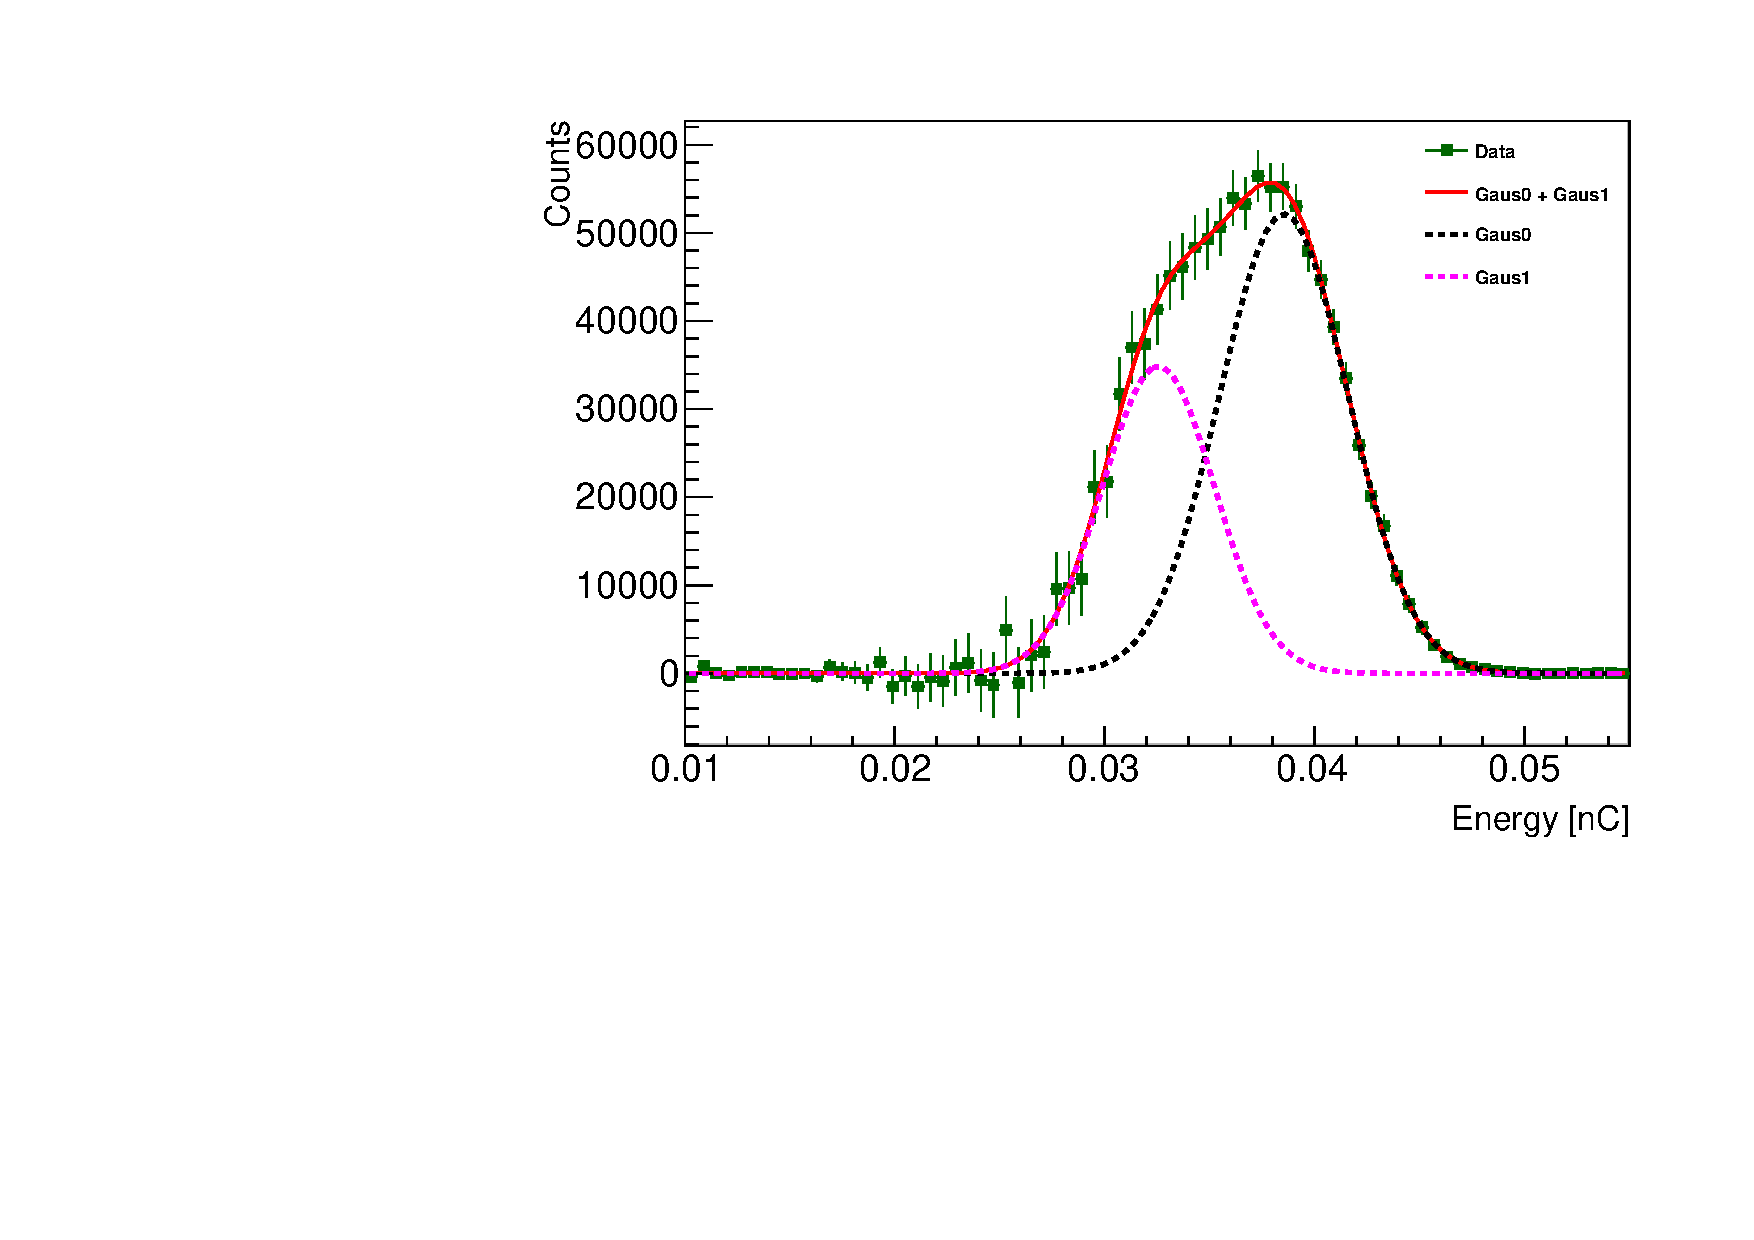
\includegraphics[width=0.6\linewidth]{tex/6-ac227-images/BNL/PoEnFit_TimeBin23_S2}
	\caption[\Po energy distribution for reference sample with two Gaussian fit]{\Po energy distribution for the reference sample, fit with a sum of two Gaussians. The total fit is seen in red, while the two Gaussians are drawn as the pink and black dashed lines.}
	\label{fig:poenfittimebin23s2}
\end{figure}

The amount of variation seen in measured rates and the \Po energy distribution indicate that the system is not repeatable and, as such, introduces significant systematic errors. 
Though the PMT and acrylic holder were glued in place, the sample vials were repeatedly removed and replaced, possibly shifting the placement of the acrylic holder and the optical grease.
If the experiment were to be repeated a more robust detector system would be needed to eliminate these systematic errors.

\begin{figure}[!t]
	\centering
	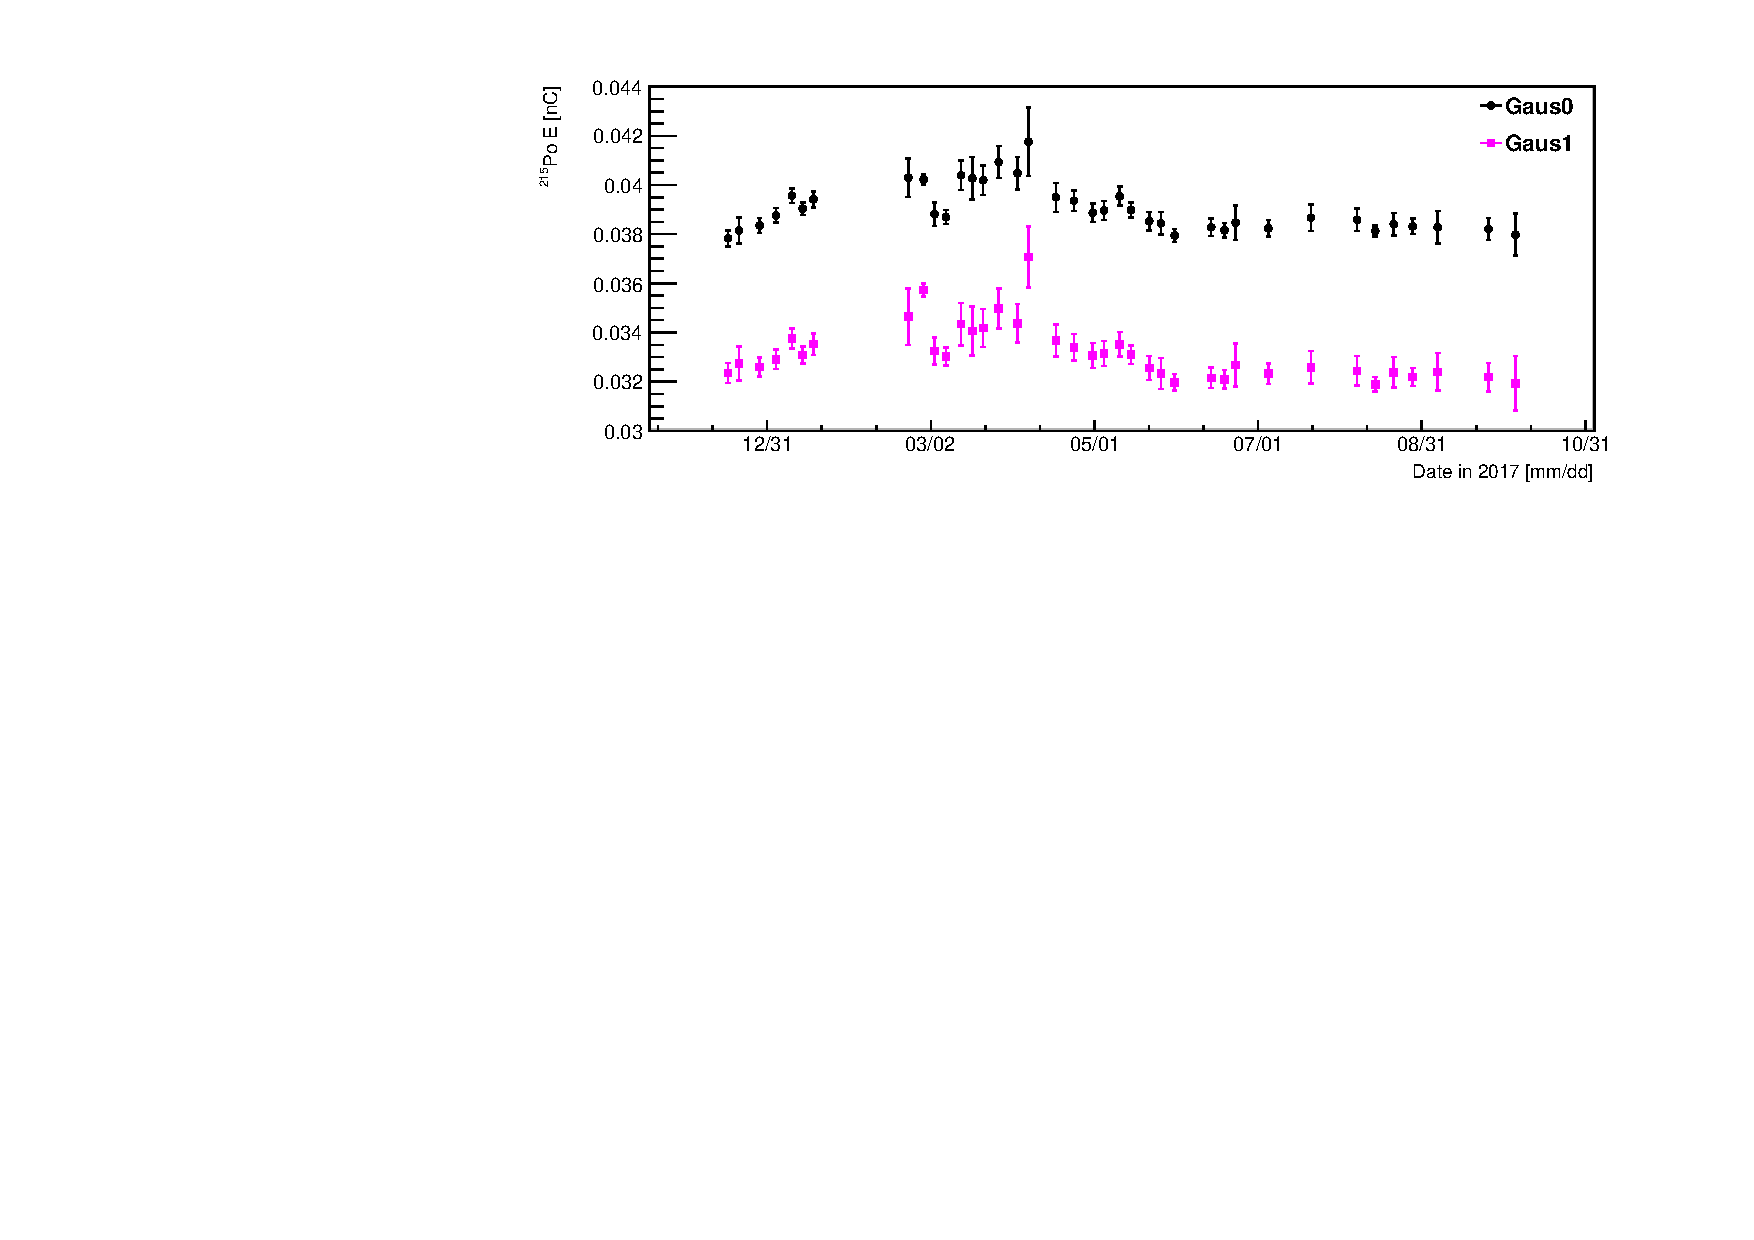
\includegraphics[width=0.8\linewidth]{tex/6-ac227-images/BNL/PoEnMeanVsTime_S2}
	\caption[\Po mean versus time for the reference sample]{The mean of the two Gaussians fit to the \Po distribution for the reference sample.}
	\label{fig:poenmeanvstimes2}
\end{figure}

\begin{figure}[!t]
	\centering
	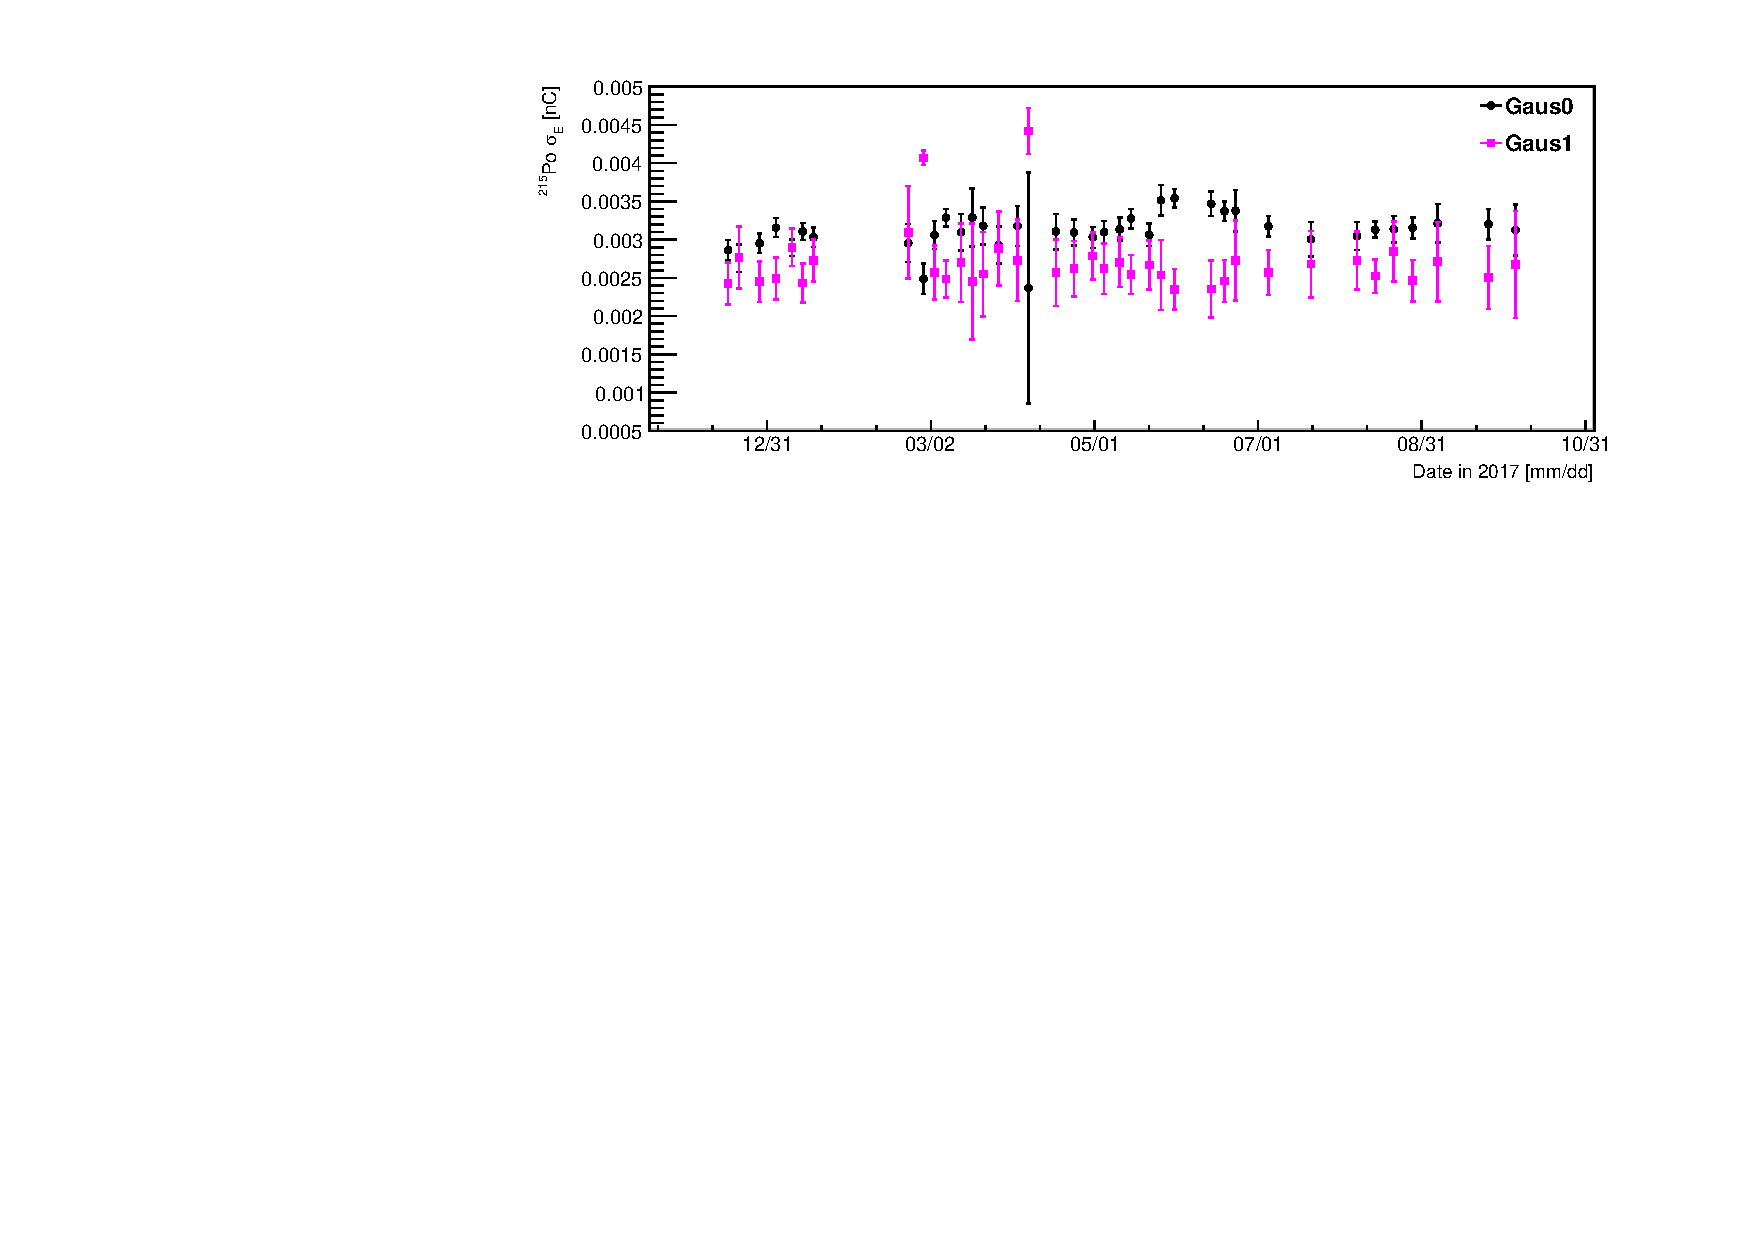
\includegraphics[width=0.8\linewidth]{tex/6-ac227-images/BNL/PoEnWidthVsTime_S2}
	\caption[\Po 1$\sigma$ width versus time for the reference sample]{The 1 $\sigma$ width of the two Gaussians fit to the \Po distributions for the reference sample.}
	\label{fig:poenwidthvstimes2}
\end{figure}

To account for these variations all material sample rates, $R_M$, were compared to the reference sample rate, $R_{ref}$.
The ratio of the rates was calculated for each time bin as
\begin{equation}
ratio = \frac{R_M}{R_{ref.}}
\end{equation}
\begin{equation}
\sigma_{ratio} = ratio \times \sqrt{\left(\frac{\sigma_{M}}{R_{M}}\right)^2+\left(\frac{\sigma_{ref.}}{R_{ref.}}\right)^2}
\end{equation}
and the results are shown in Figure~\ref{fig:relratevstimeallsamples}.
The ratio of rates versus time, for each material, were fit with a constant and a straight line, the results of which are tabulated in Tables~\ref{tab:MatFitC} and \ref{tab:MatFitLine} respectively.

Except for the case of viton (discussed in the next section) there is no clear decrease in rate observed over the six month period for any material.
Though the chi-squared results for the constant fits are not ideal, the fits to a straight line result in slopes with 50\% error to greater than 100\% error, indicating that a decrease in rate is not a good model.
Since no obvious and significant decrease was observed it was concluded that \Ac was not adsorbing onto materials and next steps were taken to include the source in the final detector.

\begin{figure}[H]
	\centering
	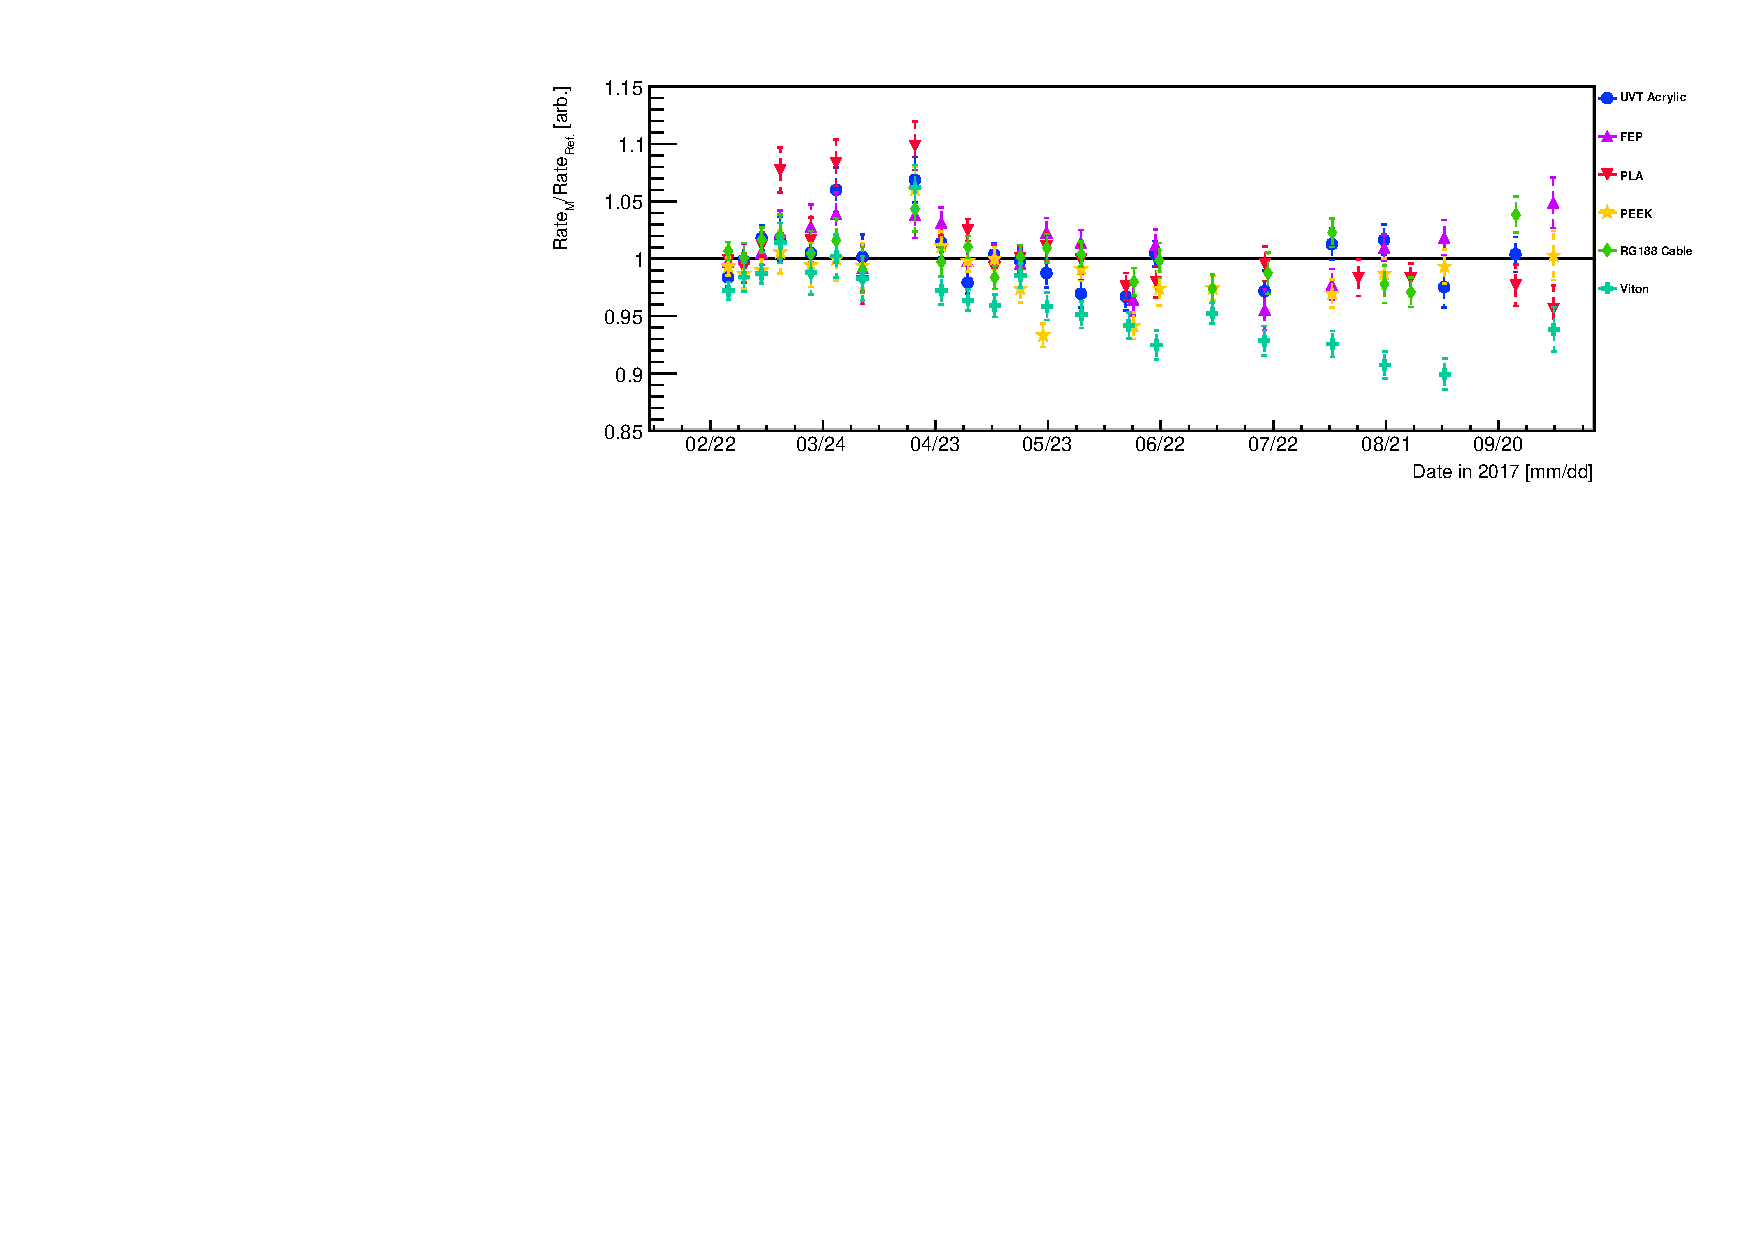
\includegraphics[width=1\linewidth]{tex/6-ac227-images/BNL/RelRateVsTime_AllSamples}
	\caption[\Ac rate for each material sample relative to the reference sample]{\Ac rate for each material sample, $M$, relative to the reference sample.}
	\label{fig:relratevstimeallsamples}
\end{figure}

\begin{table}[H]
	\centering
\begin{tabular}{|c|c|c|}
	\hline 
	\textbf{Material} & \textbf{Constant} & \textbf{$\chi^2$/NDF} \\ 
	\hline 
	UVT Acrylic  & 0.997 $\pm$ 0.003 & 56.5/20 = 2.82 \\ 
	\hline 
	FEP & 1.005 $\pm$ 0.003 & 44.1/20 = 2.21 \\ 
	\hline 
	PLA & 1.003 $\pm$ 0.003 & 80.6/20 = 4.03 \\ 
	\hline 
	PEEK & 0.985 $\pm$ 0.003 & 70.9/20 = 3.55 \\ 
	\hline 
	RG188 Cable & 1.001 $\pm$ 0.003 & 38.3/21 = 1.82 \\ 
	\hline 
	Viton  & 0.960 $\pm$ 0.002 & 136.3/21 = 6.49 \\ 
	\hline 
\end{tabular} 
\caption{The results of fitting the relative rate for each material sample with a constant.}
\label{tab:MatFitC}
\end{table}

\begin{table}[H]
	\centering
\begin{tabular}{|c|c|c|c|}
	\hline 
	\textbf{Material} & \textbf{Constant} & \textbf{Slope [ratio/yr]} & \textbf{$\chi^2/NDF$} \\ 
	\hline 
	UVT Acrylic  & 1.5 $\pm$ 0.8 & -0.01 $\pm$ 0.02 & 56.2/19 = 2.96 \\ 
	\hline 
	FEP  & 1.3 $\pm$ 0.8 & -0.005 $\pm$ 0.018 & 44.0/19 = 2.32 \\ 
	\hline 
	PLA  & 4.4 $\pm$ 0.8 & -0.07 $\pm$ 0.02 & 64.3/19 = 3.38 \\ 
	\hline 
	PEEK  & 2.9 $\pm$ 0.8 & -0.04 $\pm$ 0.02 & 65.2/19 = 3.43 \\ 
	\hline 
	RG188 Cable  & 2.3 $\pm$ 0.8 & -0.03 $\pm$ 0.02 & 35.7/20 = 1.79\\ 
	\hline 
	Viton  & 7.7 $\pm$ 0.7 & -0.14 $\pm$ 0.02 & 48.9/20 = 2.45 \\ 
	\hline 
\end{tabular} 
\caption{The results of fitting the relative rate for each material with a straight line.}
\label{tab:MatFitLine}
\end{table}

\subsubsection{Viton}

Observation of the rate of \Ac in the viton o-ring material sample vial initially indicates a decrease in rate over time, about 10\% compared to the reference vial over a six month period.
Upon further inspection, though, it becomes clear that the energy spectrum, of the Rn events in particular, shift toward the system threshold as time goes on.
This causes a loss of events, not due to adsorbance, but rather due to threshold effects.

Figure~\ref{fig:rnpoenfirstandlast} shows the \Rn and \Po energy distributions in the first and last time bins for both viton and PEEK.
It can be seen that at the last time bin the viton distributions sit against the threshold, compared to the PEEK distributions which approach but do not get close to the threshold.
To quantify this the \Rn spectrum was fit with a sum of two Gaussians and the widths versus time are shown in Figure~\ref{fig:rnenwidths8}.
It can be seen that the lower energy Gaussian becomes narrower as time goes on, indicating a loss of events due to threshold effects.
Therefore, it was concluded that the decrease in \Ac rate observed in the viton o-ring sample was due to threshold effects rather than adsorption.


\begin{figure}[H]
	\begin{subfigure}{1\linewidth}
	\centering
	\includegraphics[width=1.\linewidth]{"tex/6-ac227-images/BNL/RnPoEn_FirstAndLast_S8"}
	%\caption{}
	\label{fig:rnpoenfirstandlasts8}
\end{subfigure}
\begin{subfigure}{1\linewidth}
	\centering
	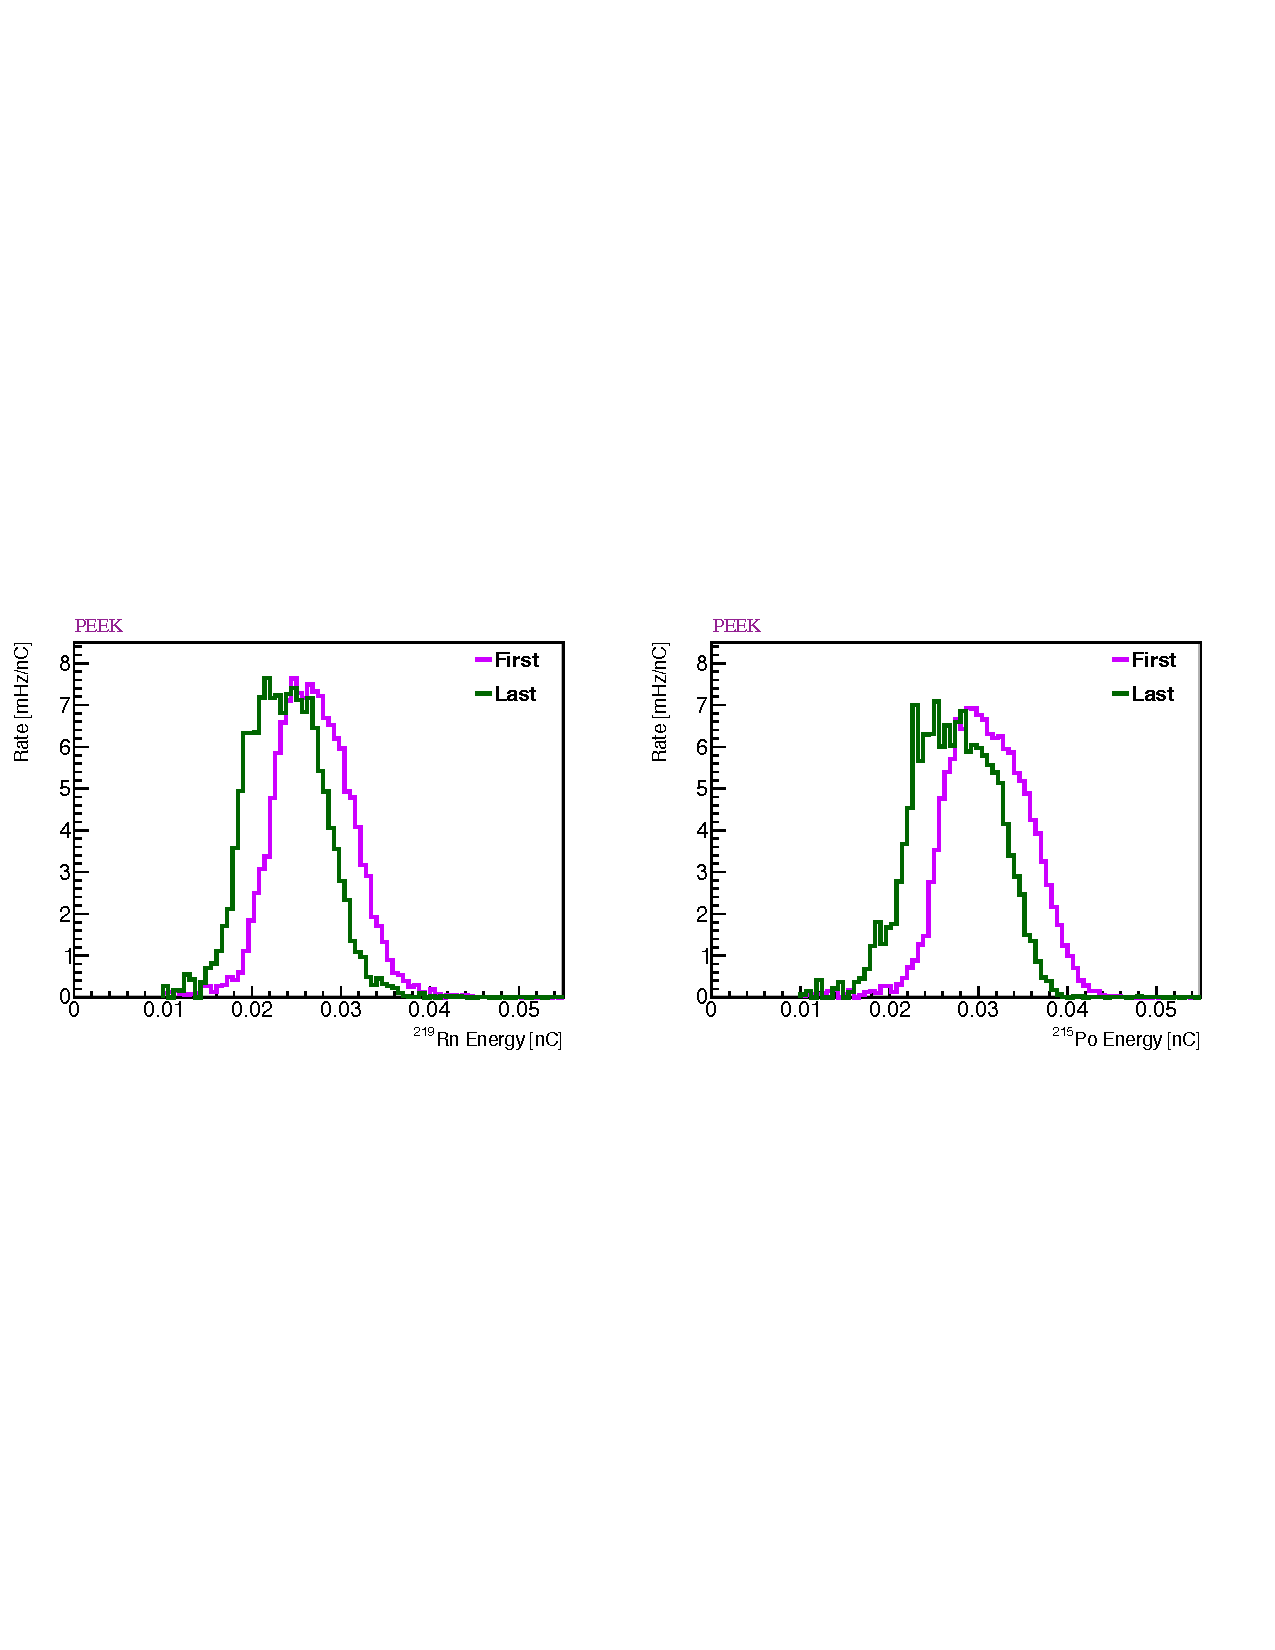
\includegraphics[width=1\linewidth]{tex/6-ac227-images/BNL/RnPoEn_FirstAndLast_S6}
	%\caption{}
	\label{fig:rnpoenfirstandlasts6}
\end{subfigure}
\caption[RnPo energy spectra for viton and PEEK at the first and last time bins]{\Rn and \Po energy spectra for both the viton o-ring (top) and PEEK (bottom) material samples during the first and last time bins.}
\label{fig:rnpoenfirstandlast}
\end{figure}

\begin{figure}[H]
	\centering
	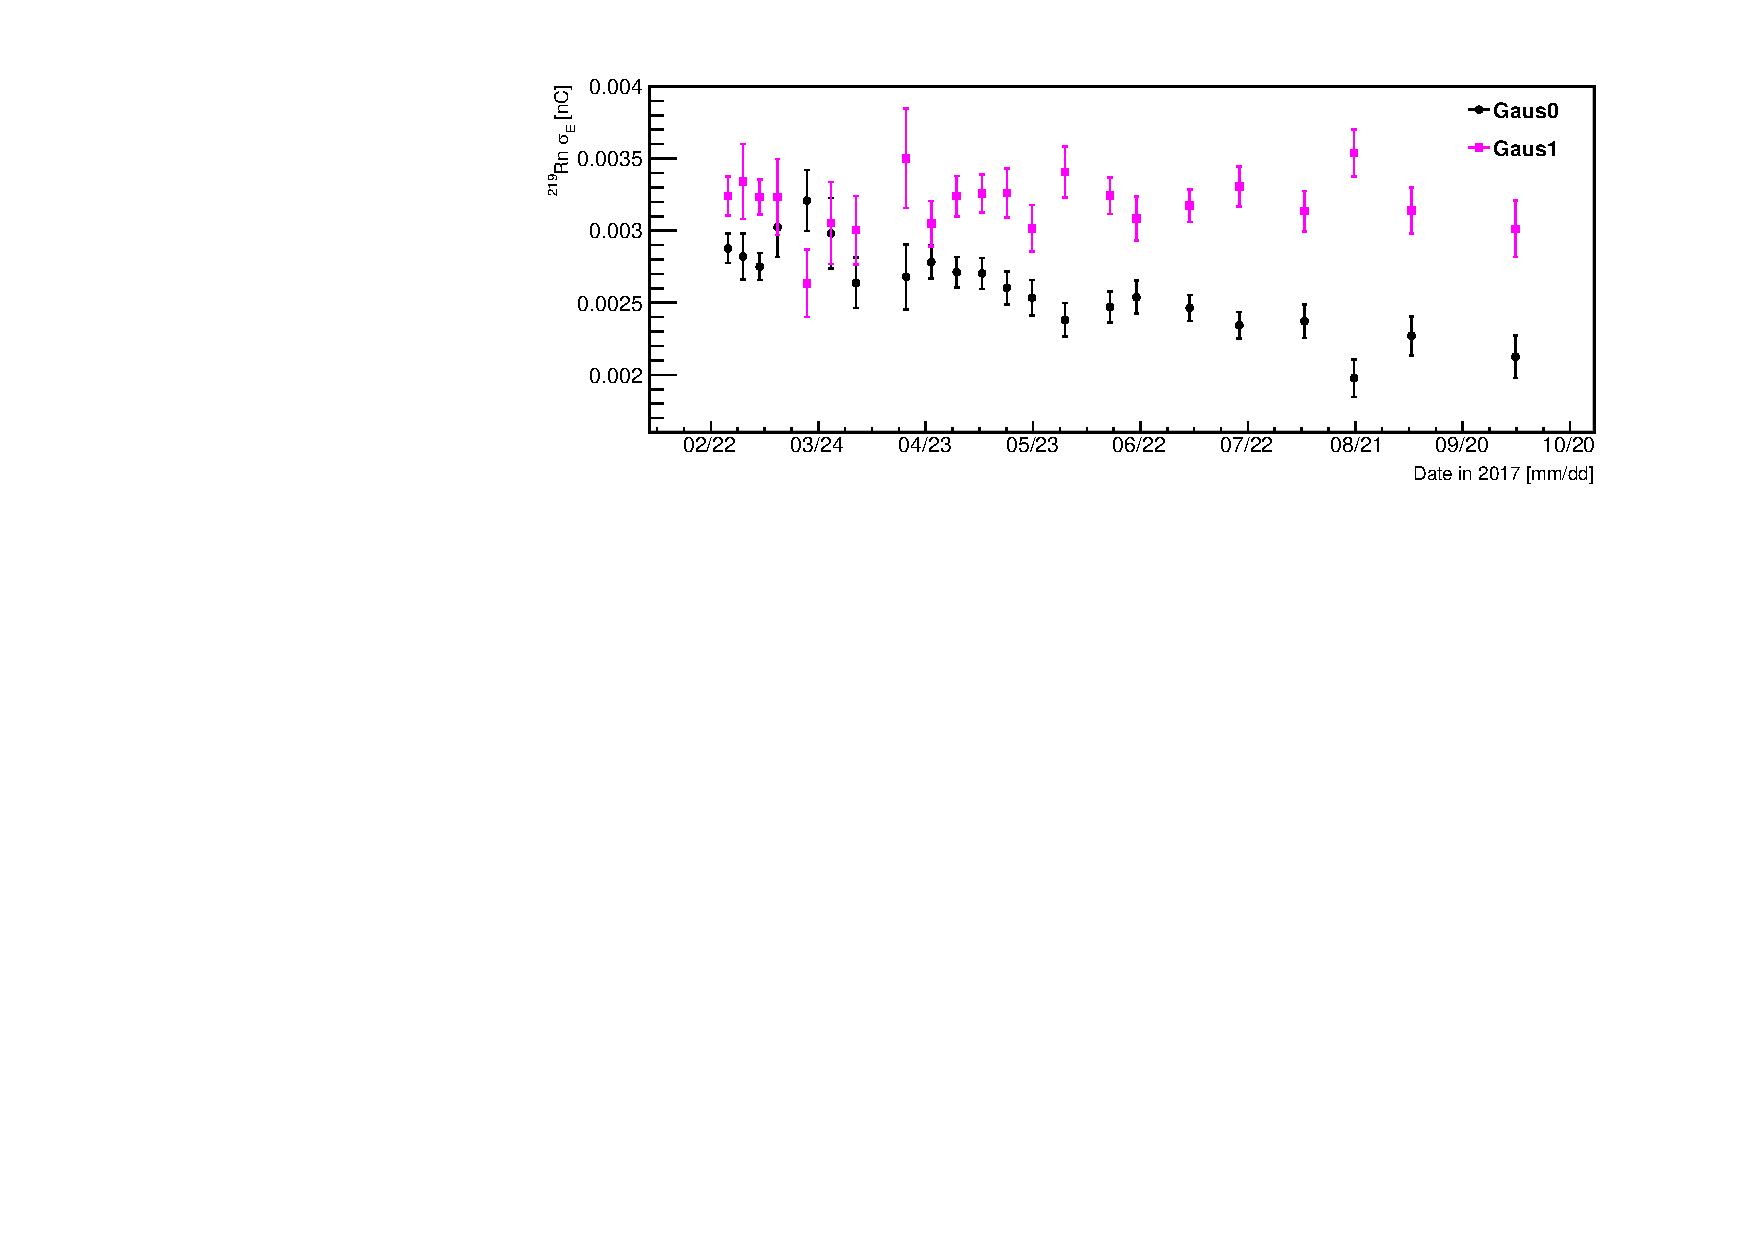
\includegraphics[width=0.9\linewidth]{tex/6-ac227-images/BNL/RnEnWidth_S8}
	\caption{The 1$\sigma$ width of two Gaussians fit to the \Rn energy spectrum versus time for the viton o-ring material sample. Black (circle): higher energy Gaussian, Magenta (square): lower energy Gaussian.}
	\label{fig:rnenwidths8}
\end{figure}



\section{\Ac in the PROSPECT AD}

Material compatibility testing determined that \Ac did not adsorb onto detector materials, confirming that it could be used as a uniformly distributed source.
It will be noted here that \Ac spiked LiLS was added to a prototype detector that consisted of two stacked segments.
This was done to determine that the \Ac did not degrade the performance of the liquid scintillator and that it did not introduce significant background.
Initial results from the prototype concluded that it did neither and provided the last step of evidence needed before addition to the full-scale detector.

\subsection{Spiking the LiLS}

After concluding that \Ac would be added to the AD, the goal was to obtain a final activity of 0.01 Bq/segment. 
Assuming a total LiLS mass of 4600 kg and an active mass of 3939 kg implies a total \Ac activity of 1.8 Bq.
The stock solution from which the LiLS would be spiked was the same stock that was used for the material studies, which had an activity of $\sim$9.13 Bq/g on December 13, 2017, the day the spiking procedure was performed.
This means that $\sim$200 mg of the stock was needed to spike the LiLS.

In order to add \Ac to the total detector, a vial of spiked LiLS was added to a 55-gallon drum of LiLS prepared previously for detector filling.
Before the detector was filled all drums were added to an ISO-tank and bubbled with nitrogen to ensure thorough mixing of the LiLS from all drums and the \Ac.

Spiking of the drum was done by adding the stock solution to an intermediate vial of production LiLS before spiking the vial that is added to the drum. 
This was done to offset the estimated 10 mg uncertainty of the balance used to weigh the vials and allows an assessment of the activity of the remaining vial.
The procedure was also repeated in a second set of vials so that both vials could be measured.

The spiking procedure was performed using four vials, V0, V1, V2, and V3.
The steps were:
\begin{enumerate}
	\item Fill all four vials with production LiLS
	\item Fill V1 and V2 with the \Ac spiked LiLS stock solution
	\item Fill V0 with solution from V1 until desired activity is reached
	\item Fill V3 with solution from V2 until desired activity is reached
	\item Empty V0 into drum of production LiLS 
\end{enumerate}
See Figure~\ref{fig:spikingprocedure} for a graphic of these steps along with Table~\ref{tab:SpikeProc} for a list of the weights of all solutions added and removed from the vials.
Filling of all vials was performed using pipettes, therefore, some drops inevitably remained in the pipette at every step.
Vials V1 and V2 were gently swirled after the addition of the \Ac spiked LiLS in an attempt to mix the solution.

\begin{figure}[!hb]
	\centering
	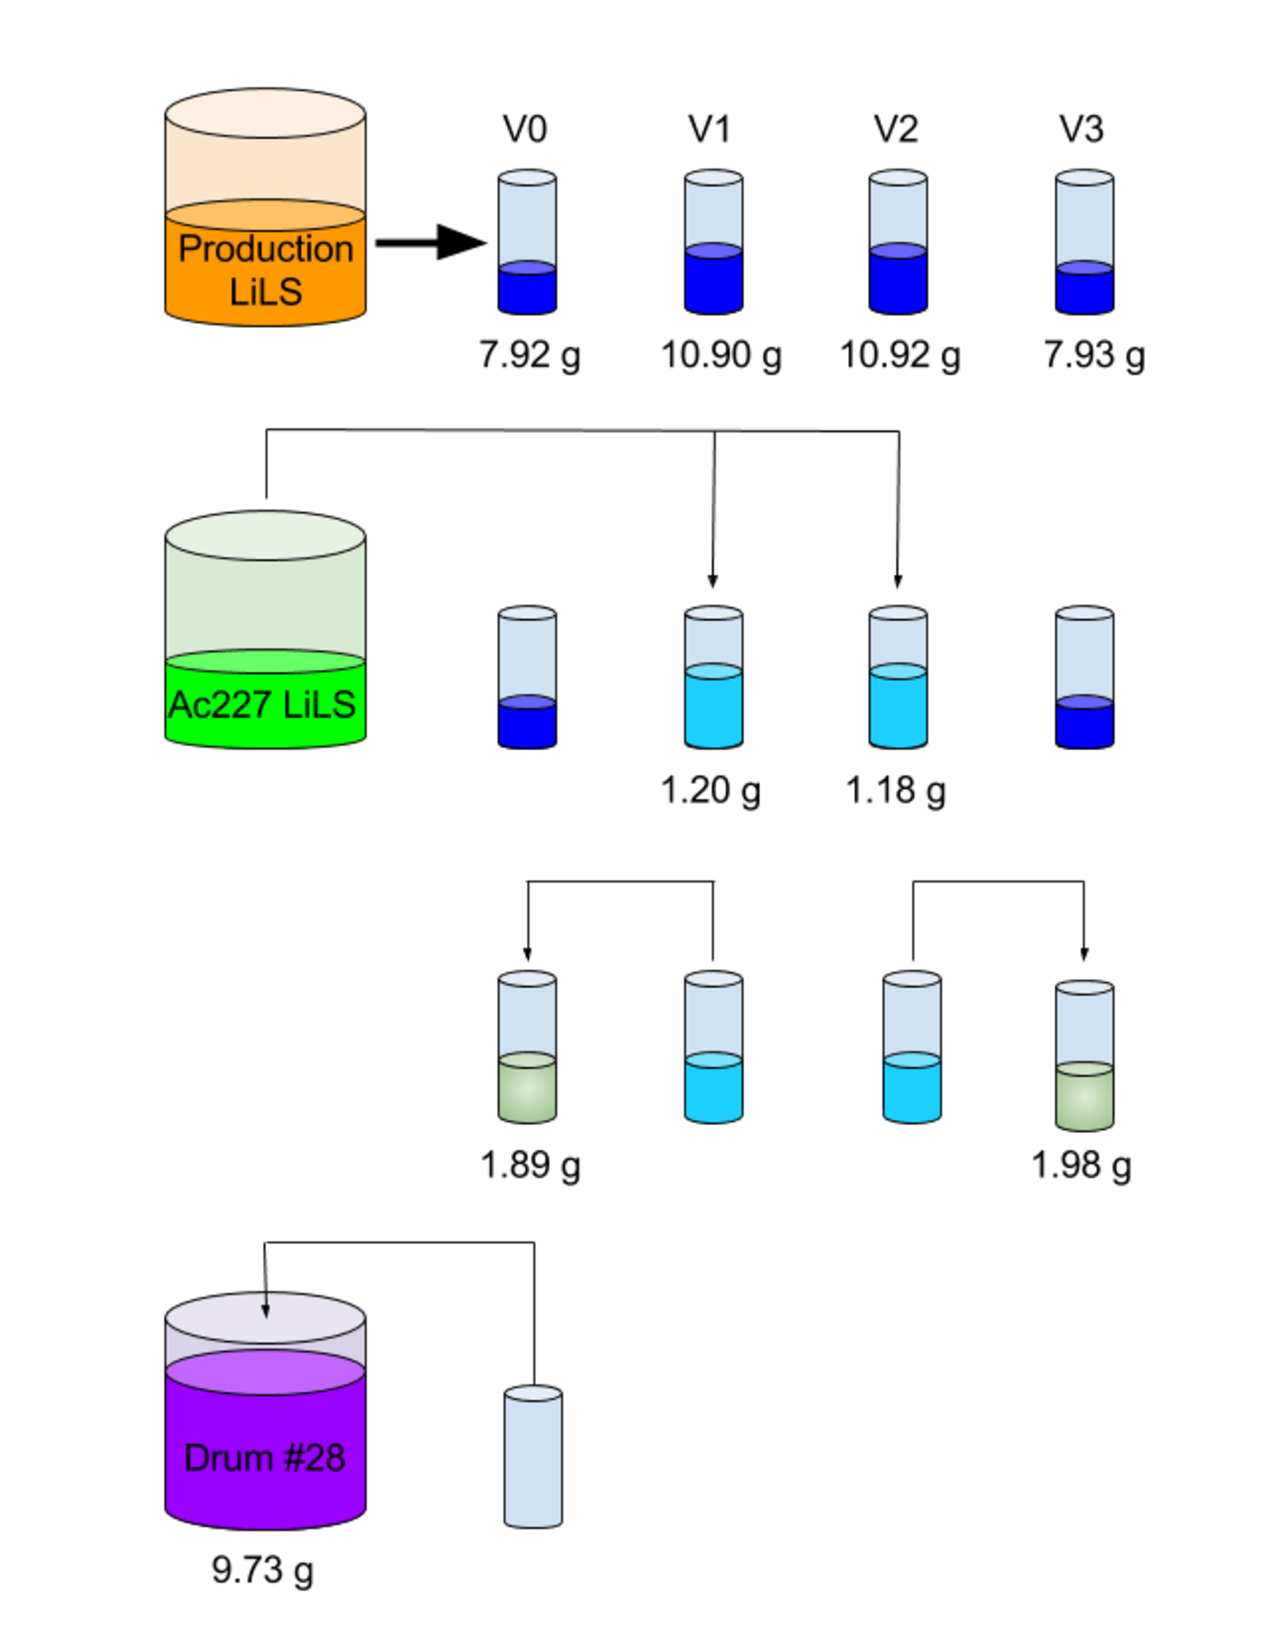
\includegraphics[width=0.5\linewidth]{tex/6-ac227-images/BNL/SpikingProcedure}
	\caption{A graphic of the procedure used to spike the drum of LiLS with \Ac for filling of the AD.}
	\label{fig:spikingprocedure}
\end{figure}

\begin{table}[!ht]
	\centering
\begin{tabular}{r|c|c|c|c}
	\hline 
	& \textbf{V0} & \textbf{V1} & \textbf{V2} & \textbf{V3} \\ 
	\hline 
	\textbf{Production LiLS added, $m_1$ (g)}  & 7.92 & 10.90 & 10.92 & 7.925 \\ 
	\hline 
	\textbf{\Ac spiked solution added, $m_2$ (g)} &  & 1.20 & 1.18 &  \\ 
	\hline 
	\textbf{Solution removed, $m_3$ (g)} &  & 2.047 & 2.09 &  \\ 
	\hline 
	\textbf{Solution added, $m_4$ (g)} & 1.885 &  &  & 1.98 \\ 
	\hline 
\end{tabular} 
\caption{The weight of all solutions added and removed from the four vials for spiking of the LiLS with \Ac for filling of the AD.}
\label{tab:SpikeProc}
\end{table}

The expected \Ac rate, $A$, in vials V0(V3) can be calculated as
\begin{equation}
	A = C~m_2 \frac{m_4}{m_1 + m_2}
\end{equation}
where $C$ is the activity of the \Ac spiked stock solution, 9.13 Bq/g, $m_1$ is the amount of production LiLS added to V1(V2), $m_2$ is the amount of the stock solution added to V1(V2), and $m_4$ is the amount of solution from V1(V2) that was added to V0(V3).
The expected rate in vials V1(V2) is calculated as 
\begin{equation}
A = C~m_2 \left(1 - \frac{m_3}{m_1 + m_2}\right)
\end{equation}
where $m_3$ is the amount of solution removed from V1(V2).
The expected \Ac activity for each vial is listed in Table~\ref{tab:SpikeExpA}.

The \Ac rate in vials V1, V2, and V3 were measured after adding V0 to the drum of LiLS.
The rate of \Ac in V3 should be similar to the rate in AD, recalling that the goal was 1.8 Bq.
A plot of the measured rates for each vial is shown in Figure~\ref{fig:ADVials}.
Each of these rates was fit with a constant, with the results of these fits listed in Table~\ref{tab:SpikeExpA}.
It can be seen that the measured rates in V1 and V2 are about 4\% higher than expectation, and the rate in V3 is about 50\% lower.
A possible explanation for this discrepancy is that the solution was not sufficiently mixed before transferring between the stock solution and the vials and between the vials themselves. 
If this experiment was to be repeated a more thorough testing of transfer procedures would need to be performed.
In conclusion, the measured rate in V3 indicates that the \Ac rate in the PROSPECT AD should be around 0.7 Hz, less than half of the initial goal.

\begin{table}
	\centering
\begin{tabular}{c|c|c}
	\hline 
	\textbf{Vial} & \textbf{Expected Activity [Bq]} & \textbf{Measured Rate [Hz]} \\ 
	\hline 
	V0 & 1.71 & \\ 
	\hline 
	V1 & 9.10 &  9.48 $\pm$ 0.04  \\ 
	\hline 
	V2 & 8.91 & 9.38 $\pm$ 0.06\\ 
	\hline 
	V3 & 1.76 & 0.696 $\pm$ 0.001 \\ 
	\hline 
\end{tabular} 
\caption{Expected and measured \Ac activity in vials prepared for spiking the LiLS. }
\label{tab:SpikeExpA}
\end{table}

\begin{figure}[H]
	\centering
\begin{subfigure}{1\linewidth}
	\centering
	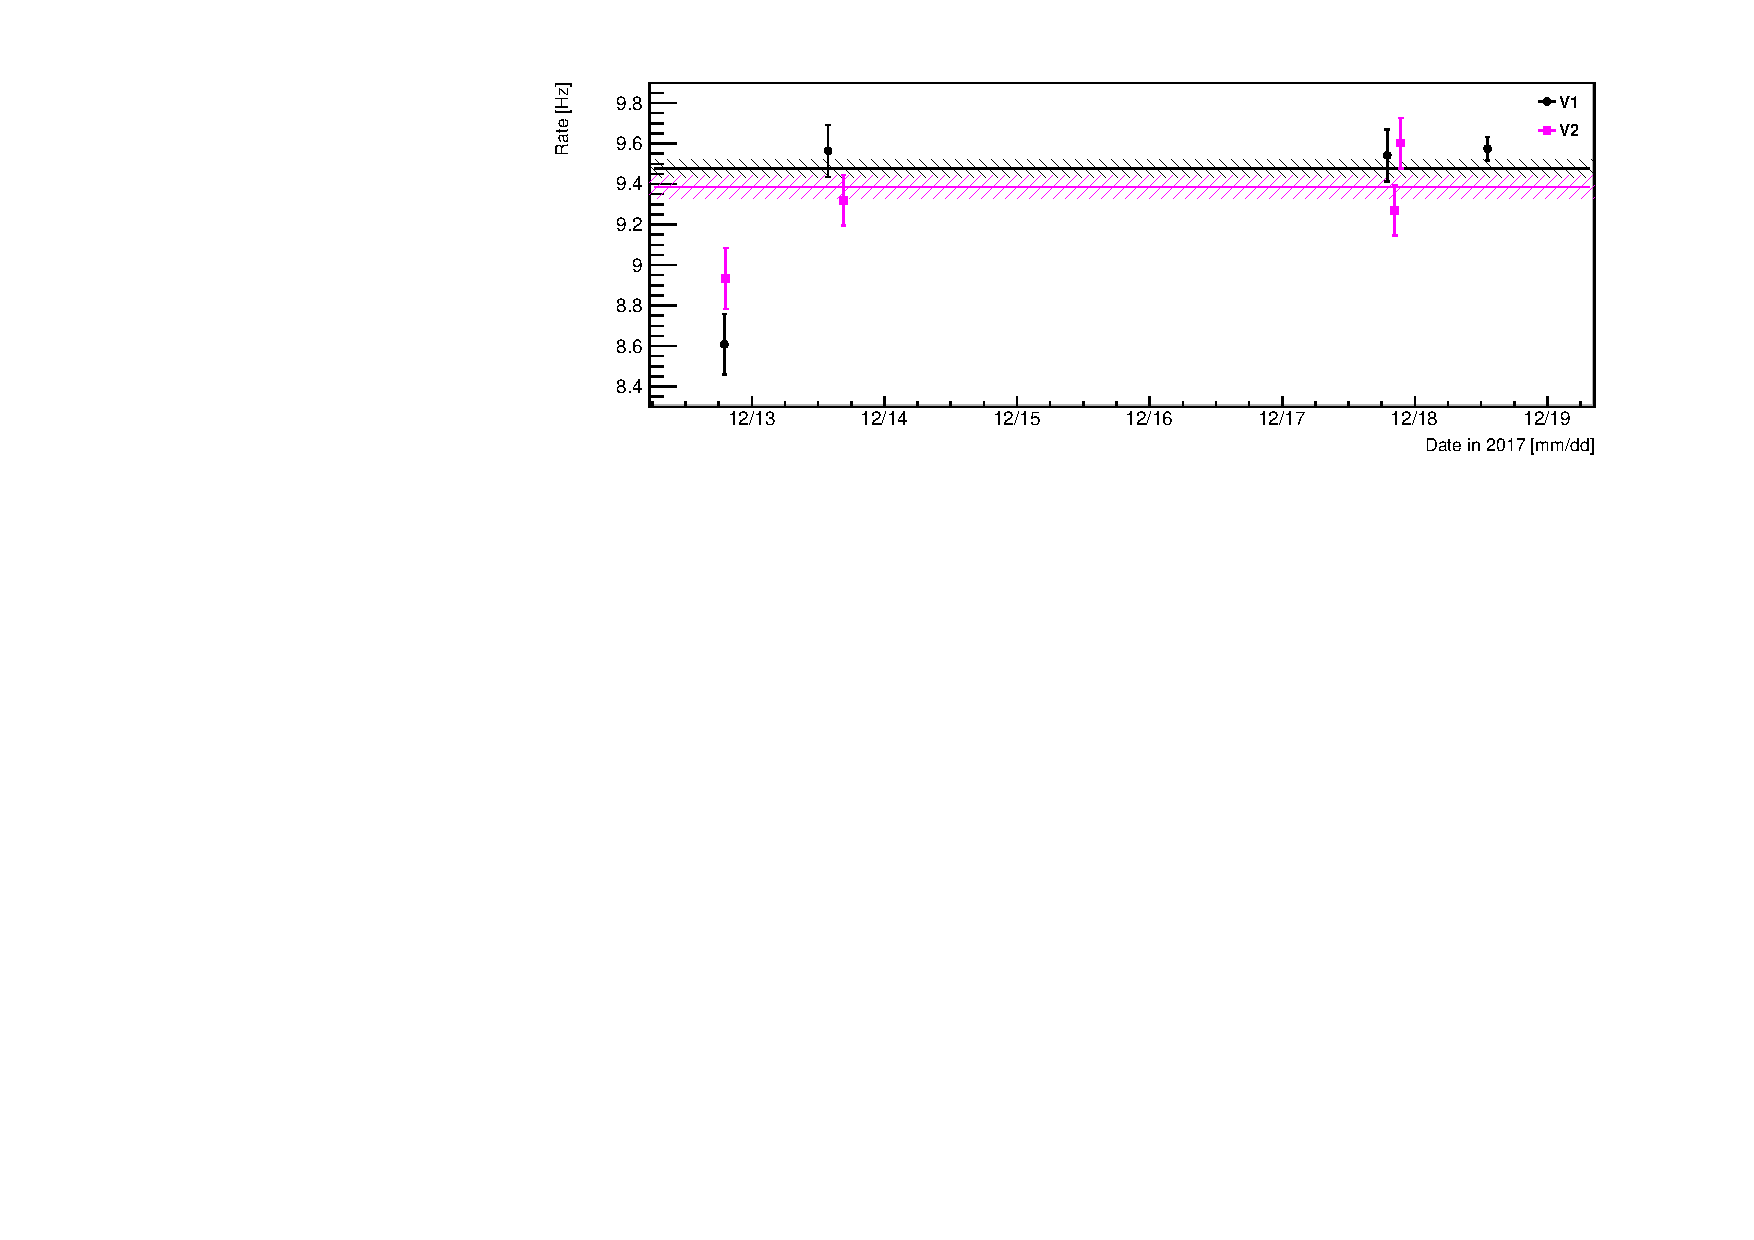
\includegraphics[width=1\linewidth]{tex/6-ac227-images/BNL/AD_Rates}
	%\caption{}
	\label{fig:adrates}
\end{subfigure}
\begin{subfigure}{1\linewidth}
	\centering
	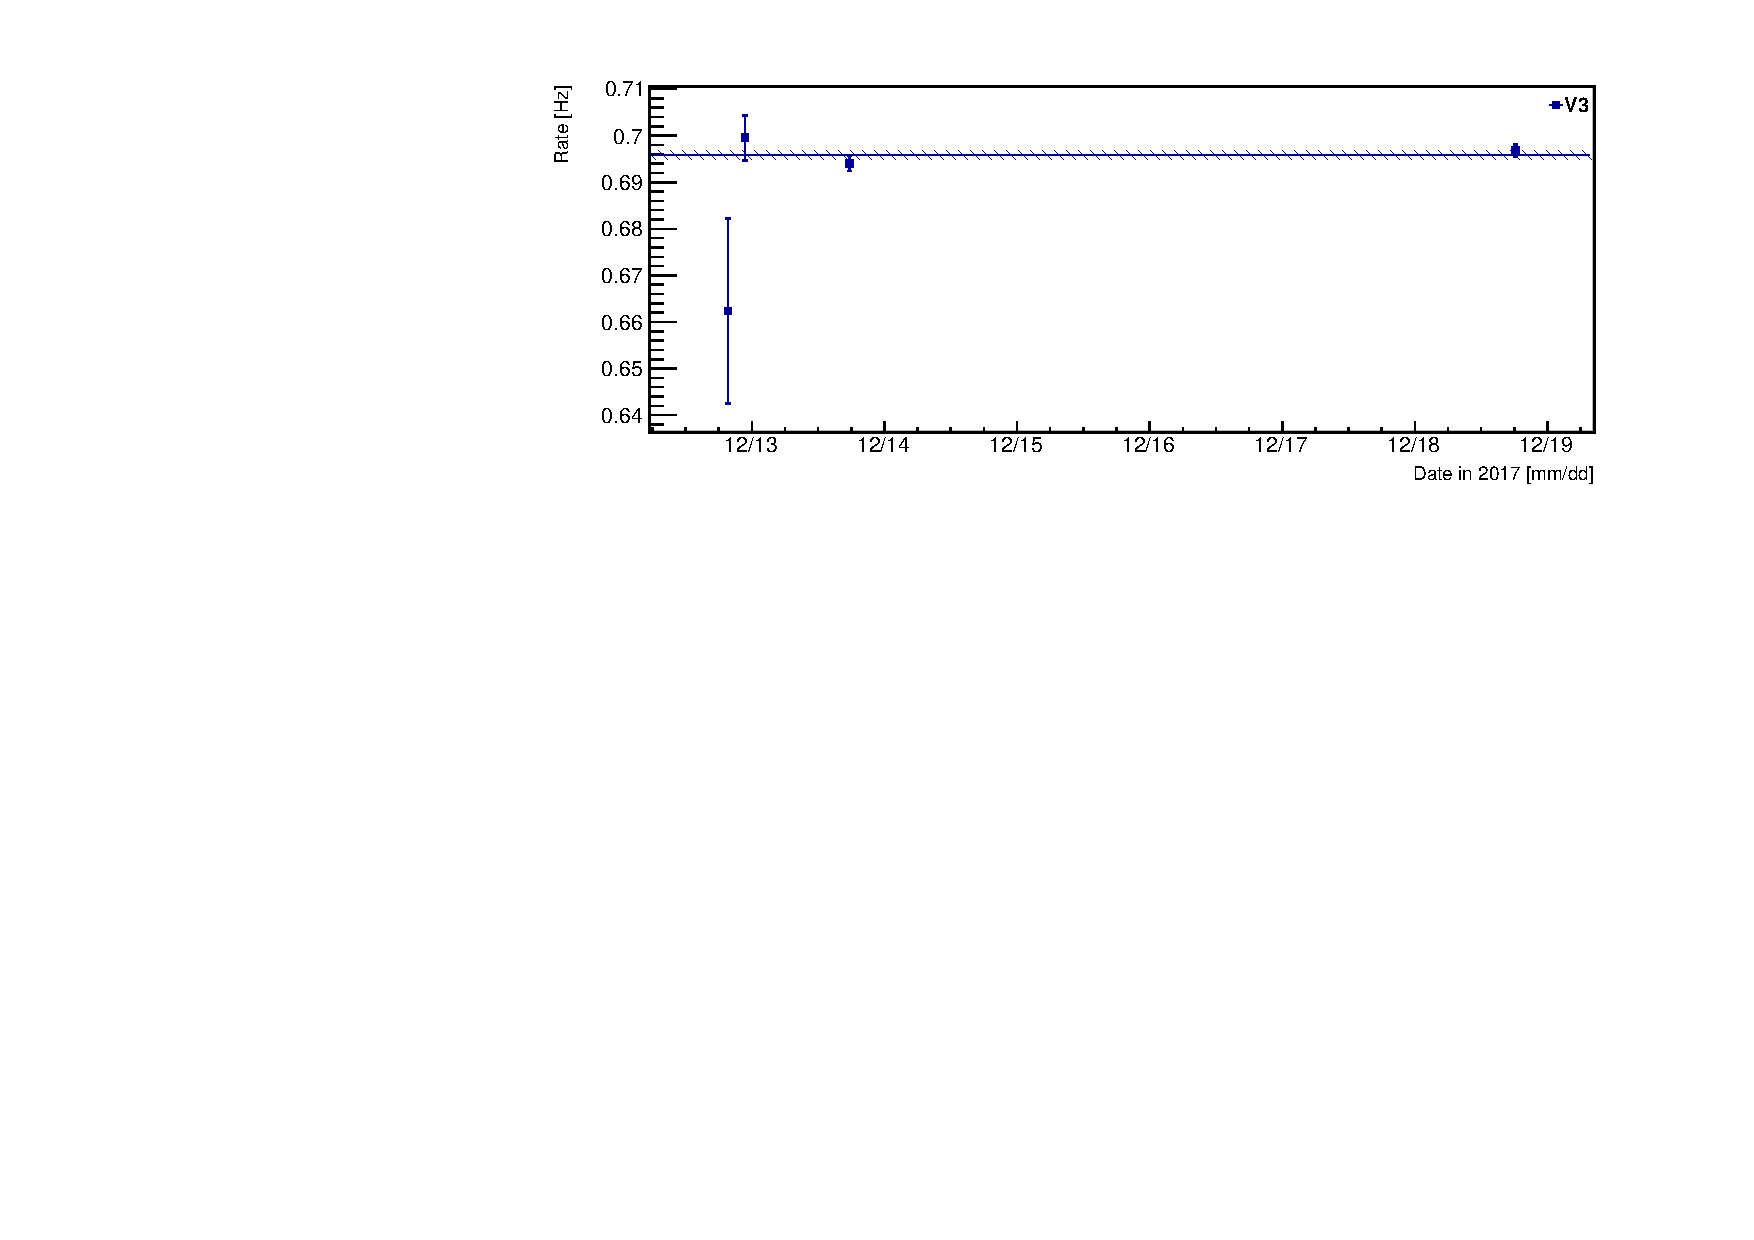
\includegraphics[width=1\linewidth]{tex/6-ac227-images/BNL/AD_RateV3}
	%\caption{}
	\label{fig:adratev3}
\end{subfigure}
\caption{Measured \Ac rates of vials used in the procedure performed to add \Ac to the LiLS of the PROSPECT AD. Top: intermediate vials V1 and V2. Bottom: V3, filled in the same method as the vial that was added to the drum of LiLS. All rates were fit with a constant, the results drawn as solid lines with hashed lines representing the error.}
\label{fig:ADVials}
\end{figure}


\subsection{Data Set}

PROSPECT began taking data in March 2018.
The data set used for the \Ac analysis runs from March 5, 2018 - October 6, 2018, with a break from March 31, 2018 - April 17, 2018 when the detector was off for maintenance. 
The total runtime is 4048.9 hrs, with 4011.7 hrs of livetime data.
2293.7 hrs of the runtime is reactor on data, and 1755.2 hrs of reactor off. 

During the data collection period used for this analysis, several PMTs exhibited abnormal behavior, including current instabilities, and are no longer in operation.
Preliminary theories for the cause of this are that LiLS leaked into the PMT housings and damaged the voltage dividers, but this has yet to be confirmed. 
To account for this all segments that `turned off' during the data period are excluded in this analysis. 
The result is 90 active segments, as shown in Figure~\ref{fig:segments}.

\begin{figure}[h]
	\centering
	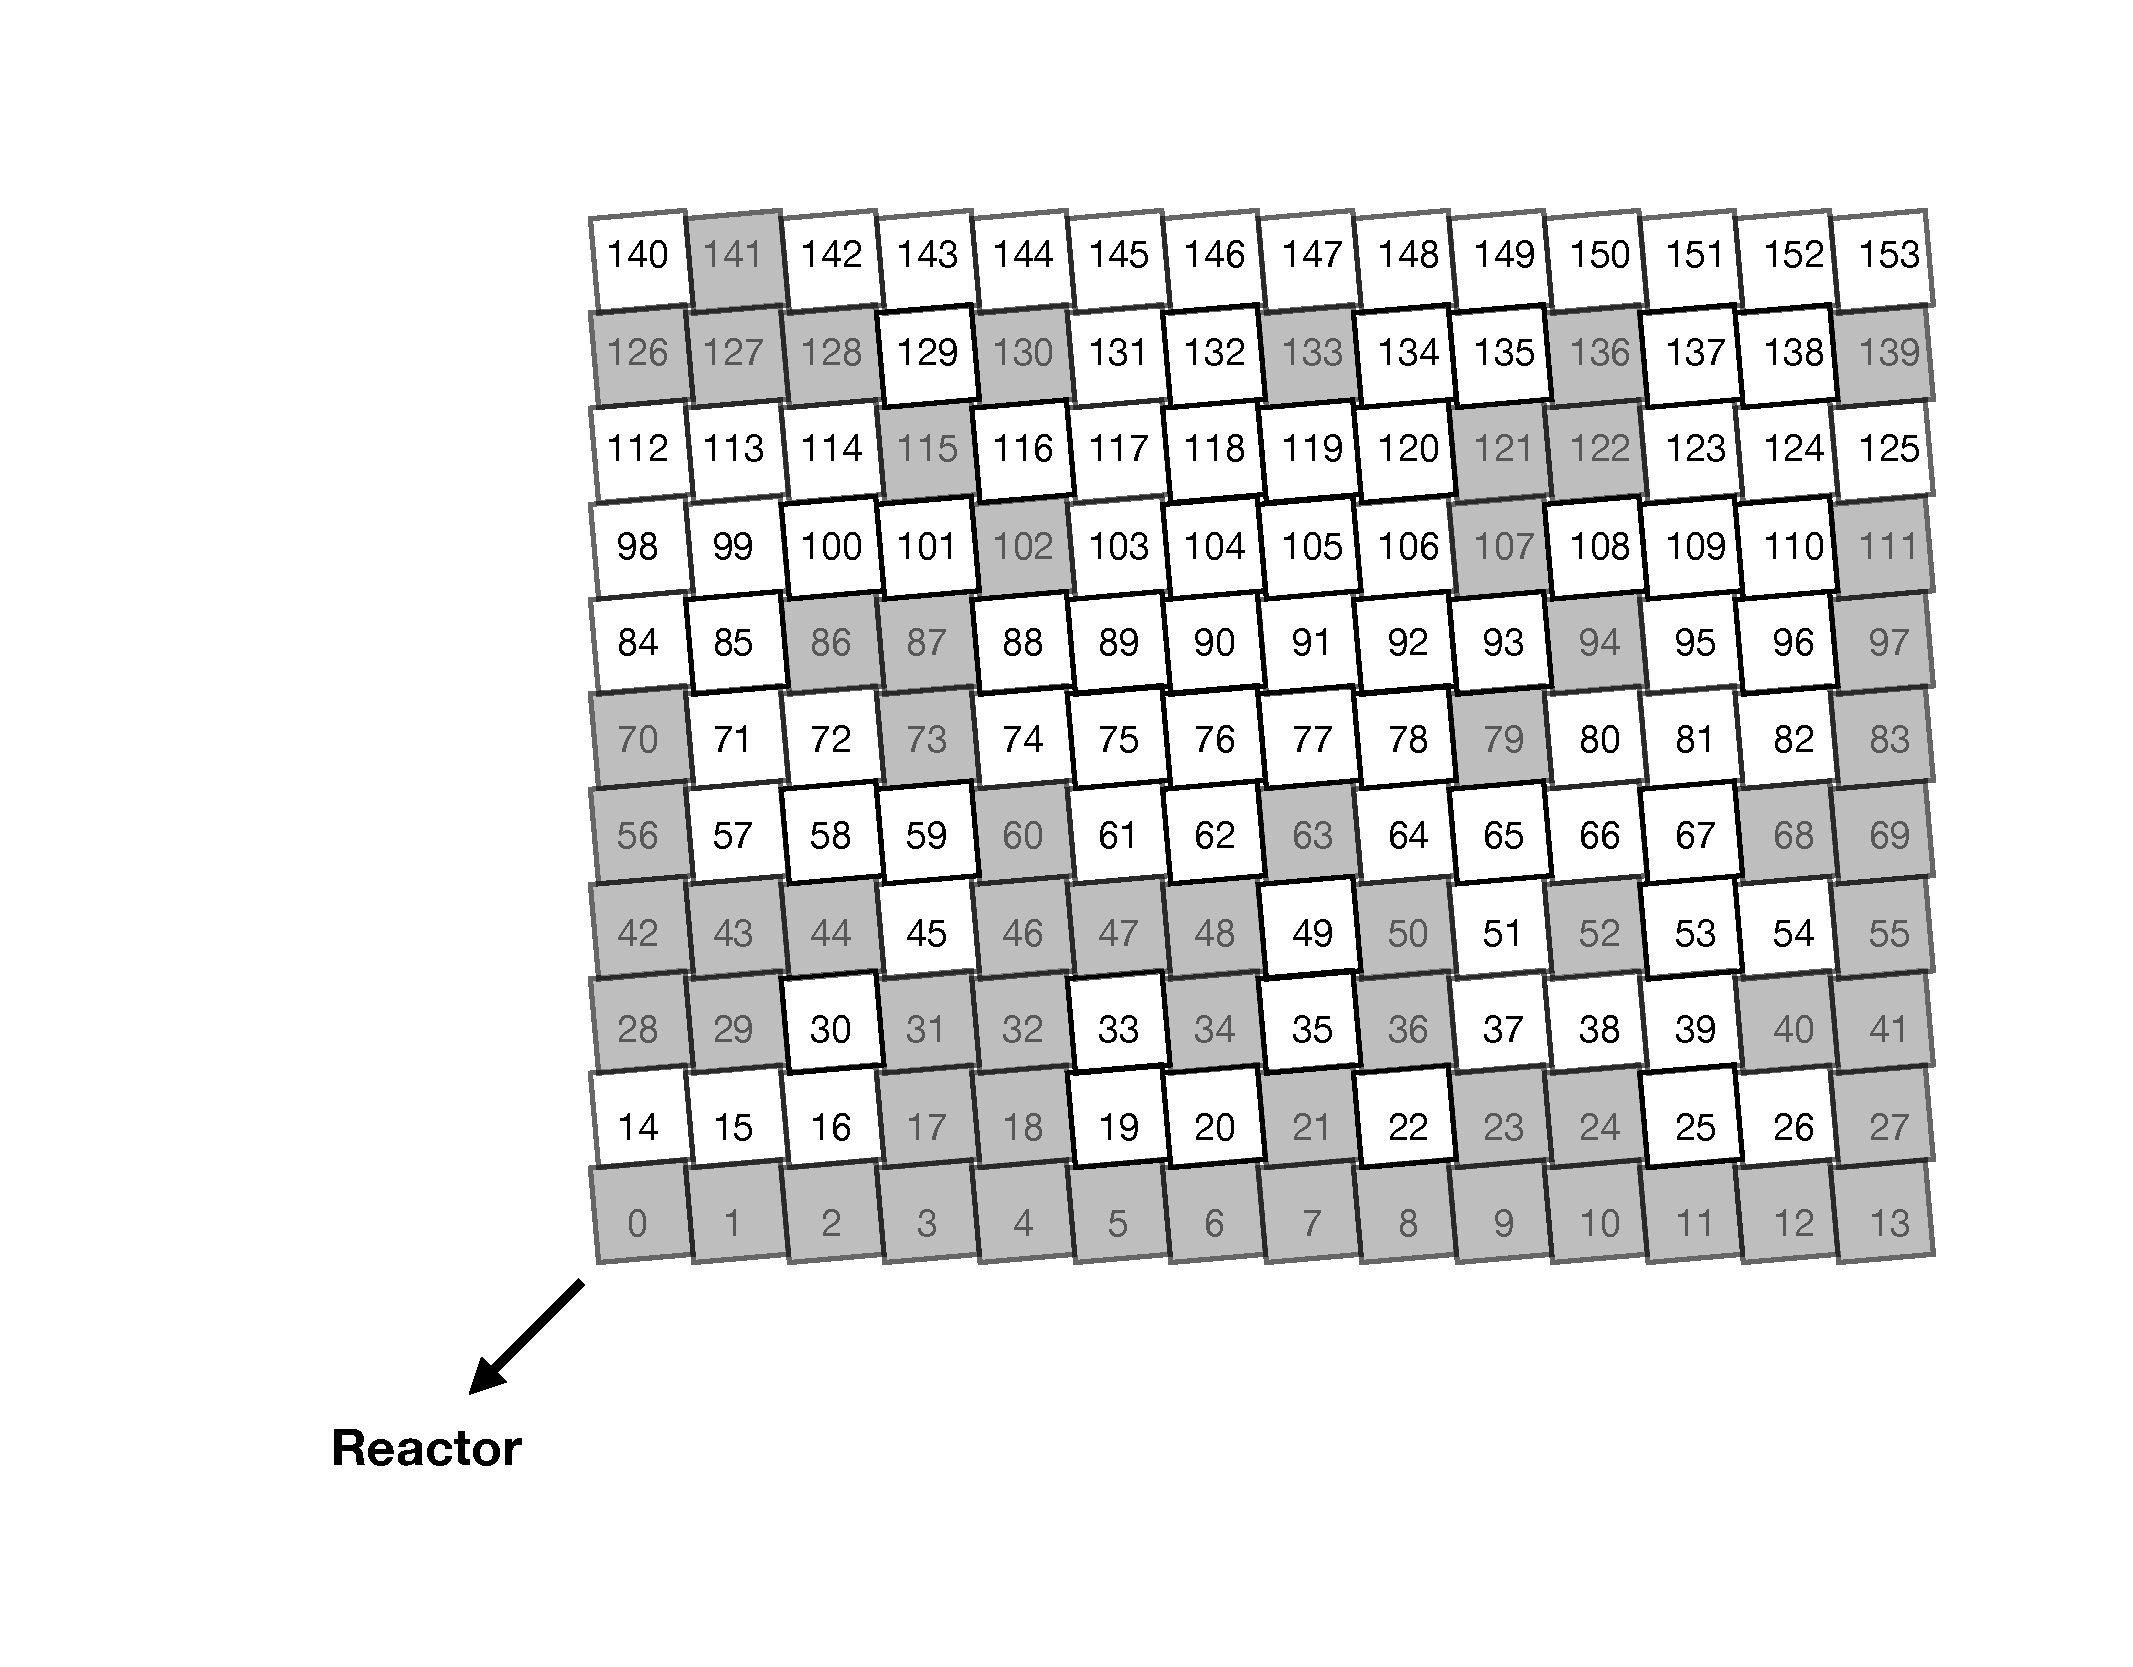
\includegraphics[width=0.7\linewidth]{tex/6-ac227-images/AD_DataSet/Segments}
	\caption{Graphic of 154 segments of the PROSPECT AD. Grayed out segments are those that `turned off' during the data period and are excluded in this analysis.}
	\label{fig:segments}
\end{figure}


\subsection{Event Selection}

RnPo events in the PROSPECT detector were found by looking at event clusters.
A cluster is defined as a collection of events that occur within 20 ns of each other.
Time coincident events were found by first looking for delay (Po) events. 
It was required that these events existed in a single multiplicity cluster and passed broad energy and PSD cuts outlined in Table~\ref{tab:RnPoCuts}.

Coincident prompt events were found by looking in a 5$\tau$ time window before the delay event, where $\tau$ is the lifetime of \Po, 2.57 ms.
It was required that the highest energy event in a given cluster in that time window occurred in the same segment as the delay event and passed the energy and PSD cuts in Table~\ref{tab:RnPoCuts}.
The distance between the prompt and delay event was also required to be less than 250 mm. 
Accidental prompt events were found by looking in a 5$\tau$ time window offset 10$\tau$ before the delay event. 
The same cuts applied to coincidental prompt events were applied to accidental prompt events.

\begin{table}[!t]
	\centering
\begin{tabular}{c|c}
	\hline 
	Prompt Energy & 0.48 $<$ E $<$ 1.18 MeVee \\ 
	\hline 
	Delay Energy & 0.61 $<$ E $<$ 1.18 MeVee \\ 
	\hline 
	PSD & 0.16 $<$ PSD $<$ 0.36 \\ 
	\hline 
	$\Delta z = |z_{\textrm{delay}} - z_{\textrm{prompt}}|$ & $\Delta z < 250$ mm  \\ 
	\hline 
	$\Delta t = t_{\textrm{delay}} - t_{\textrm{prompt}}$ & $\Delta t < 5\tau$ ms \\ 
	\hline 
\end{tabular} 
\caption{Broad cuts used to find RnPo events, where $\tau$ is the lifetime of \Po, 2.57 ms.}
\label{tab:RnPoCuts}
\end{table}

In addition to energy, PSD, and position cuts a pileup veto was applied to all events.
At the time of a trigger event all boards are signaled to begin a 592 ns acquisition window. 
Events arriving at the end of this window do not re-trigger the data acquisition system, thus causing truncated waveforms.
In order to avoid using these truncated events, any cluster preceded by another cluster in a 800 ns window is vetoed. 

The broad energy and PSD cuts listed in Table~\ref{tab:RnPoCuts} are applied on a first pass analysis of the PROSPECT data.
Changes in detector performance over time, including decreasing energy resolution and PSD, required a second pass of the data, in which the lower bounds of the energy and PSD cuts were changed to be 4$\sigma$ lower than the mean of the distributions for a given time bin or segment.
The PSD versus energy and \Po energy versus \Rn energy distributions, after accidental subtraction, can be seen in Figure~\ref{fig:RnPoPSDEn}.

\begin{figure}[H]
	\centering
	\begin{subfigure}{0.5\linewidth}
		\centering
		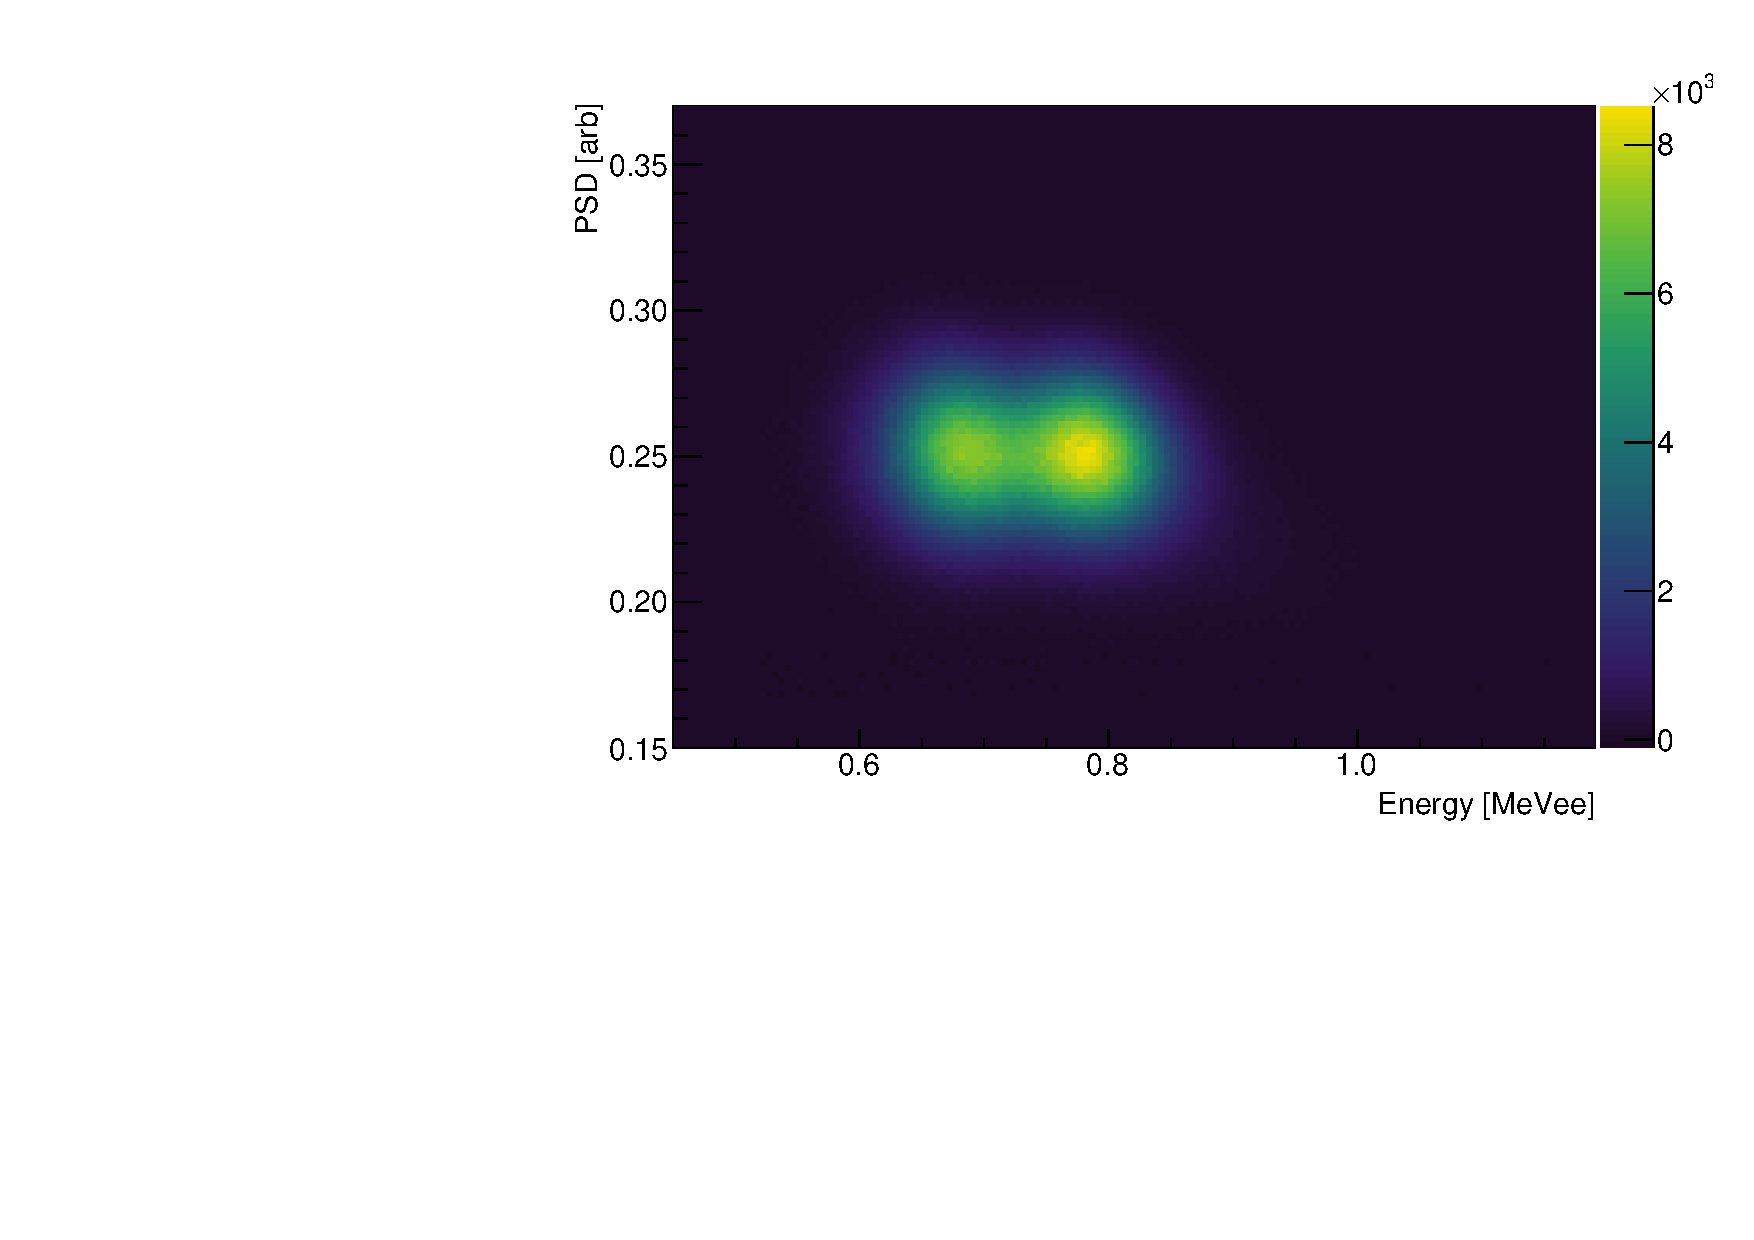
\includegraphics[width=0.8\linewidth]{tex/6-ac227-images/AD_EventSelection/RnPoPSDvsEn_AllCellsAllTime_Time0}
		\caption{RnPo PSD versus Energy.}
		\label{fig:rnpopsdvsentimebin0}
	\end{subfigure}\hspace{0cm}%
	\begin{subfigure}{0.5\linewidth}
		\centering
		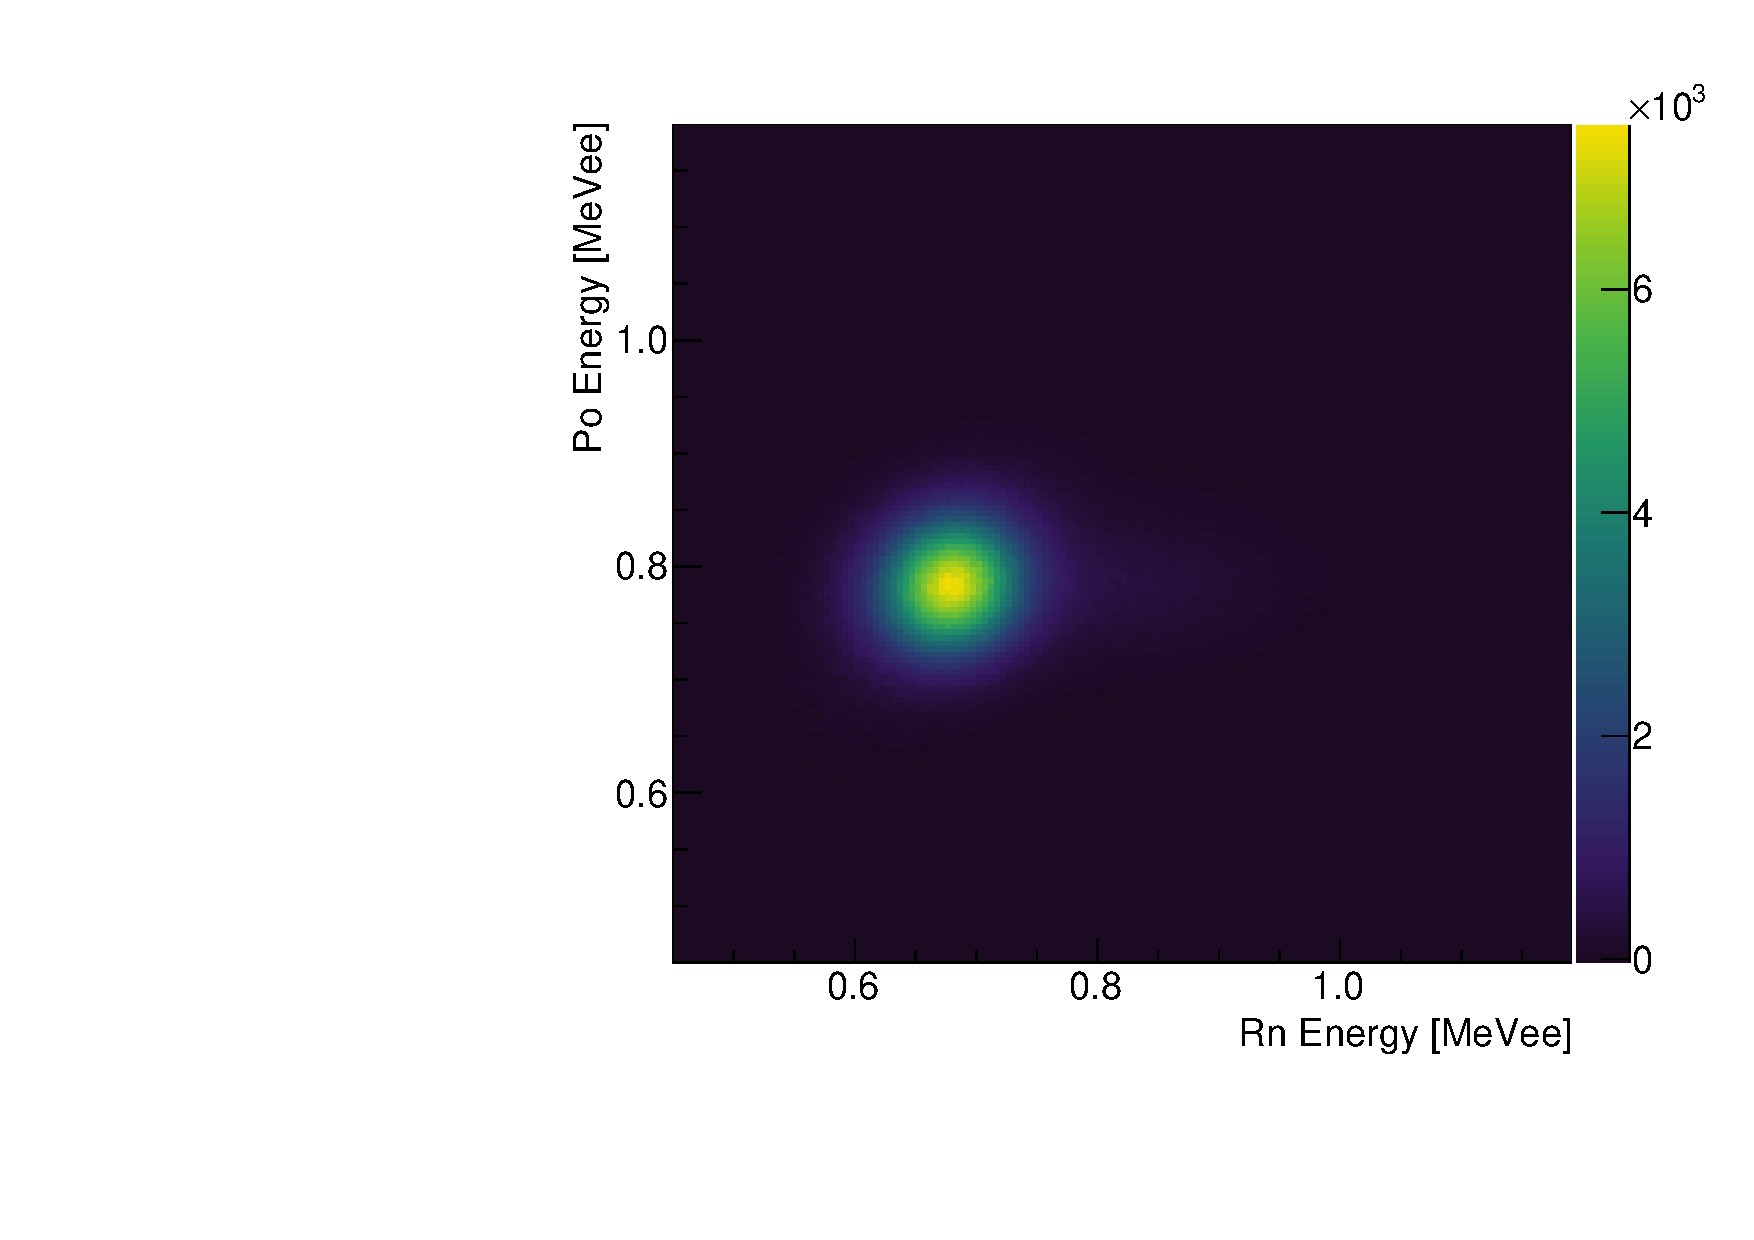
\includegraphics[width=0.6\linewidth]{tex/6-ac227-images/AD_EventSelection/PoEnvsRnEn_AllCellsAllTime_Time0}
		\caption{\Po energy versus \Rn energy.}
		\label{fig:poenvsrnentimebin0}
	\end{subfigure}
	\caption{RnPo distributions for all cells integrated over all time.}
	\label{fig:RnPoPSDEn}
\end{figure}

\subsection{Rate Calculation}

The \Ac rate per segment, or for a given time period, is found by fitting the background subtracted $\Delta t$ distribution, where $\Delta t = t_{\textrm{delay}} - t_{\textrm{prompt}}$, with
\begin{equation}
	f(t) = Ne^{-t/\tau}
	\label{eq:dtexp}
\end{equation}
where $N$ and $\tau$, the lifetime of \Po, are allowed to vary.
For an example of these distributions and fit for a typical segment see Figure~\ref{fig:rnpodtseg76}.
The rate is then calculated as
\begin{equation}
	R = \frac{N~\tau}{\Delta t\textrm{-bin-width}\times\textrm{livetime}\times\textrm{efficiency}}
\end{equation}
\begin{equation}
	\sigma_R = R \times \sqrt{\left(\frac{\sigma_N}{N}\right)^2 + \left(\frac{\sigma_\tau}{\tau}\right)^2  +  \frac{2\sigma_{N\tau}}{N\tau} + \left(\frac{\sigma_{eff.}}{eff.}\right)^2}
\end{equation}
where $N$ and $\tau$ are results of the $\Delta t$ fit.

\begin{figure}[!b]
	\centering
	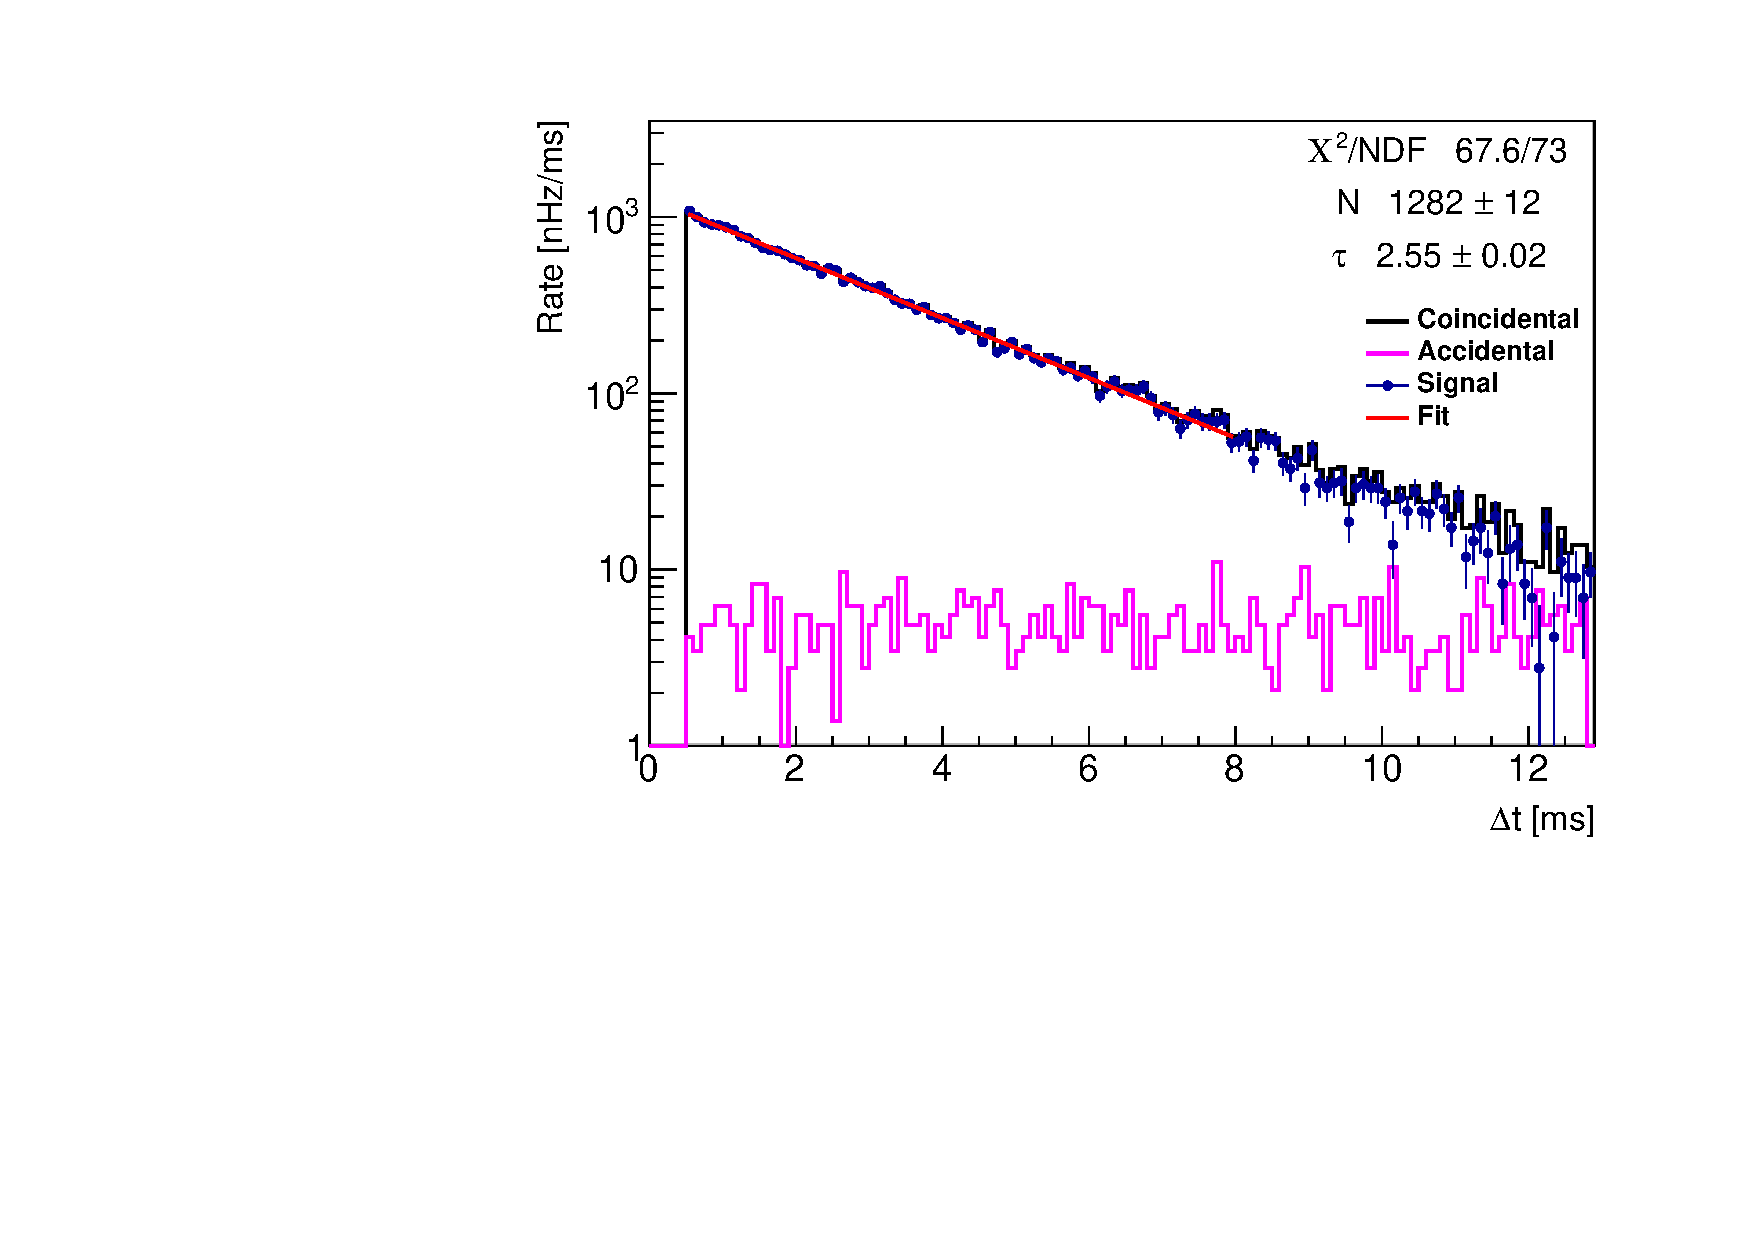
\includegraphics[width=0.7\linewidth]{tex/6-ac227-images/AD_RateCalc/RnPoDt_Seg76}
	\caption{Coincidental (black), accidental (magenta), and background subtracted (blue) $\Delta t$ distributions for a typical segment integrated over all time. A fit of Equation~\ref{eq:dtexp} to the background subtraction distribution is shown in red along with its results.}
	\label{fig:rnpodtseg76}
\end{figure}

The uncorrected livetime is calculated, for each data run, as the time from the beginning of the run to the time of the last delay candidate event. 
This is summed for all analyzed runs. 
This livetime is corrected for the dead time introduced by the pileup veto.
This correction is calculated as the number of clusters, $NClusts$, times the pileup veto time, 800 ns.
Figure~\ref{fig:vetotimevstime} shows the dead time, as a fraction of livetime, versus time.
Because the veto is applied to both prompt and delay candidates the livetime is corrected with 2$\times$ the dead time as
\begin{equation}
	\textrm{livetime} = \sum(t_{\textrm{finalPo}} - t_0) - 2.0 \times NClusts \times 800\textrm{ns}
\end{equation}
When measuring the rate per segment the same livetime is applied to all segments. 

\begin{figure}[!t]
	\centering
	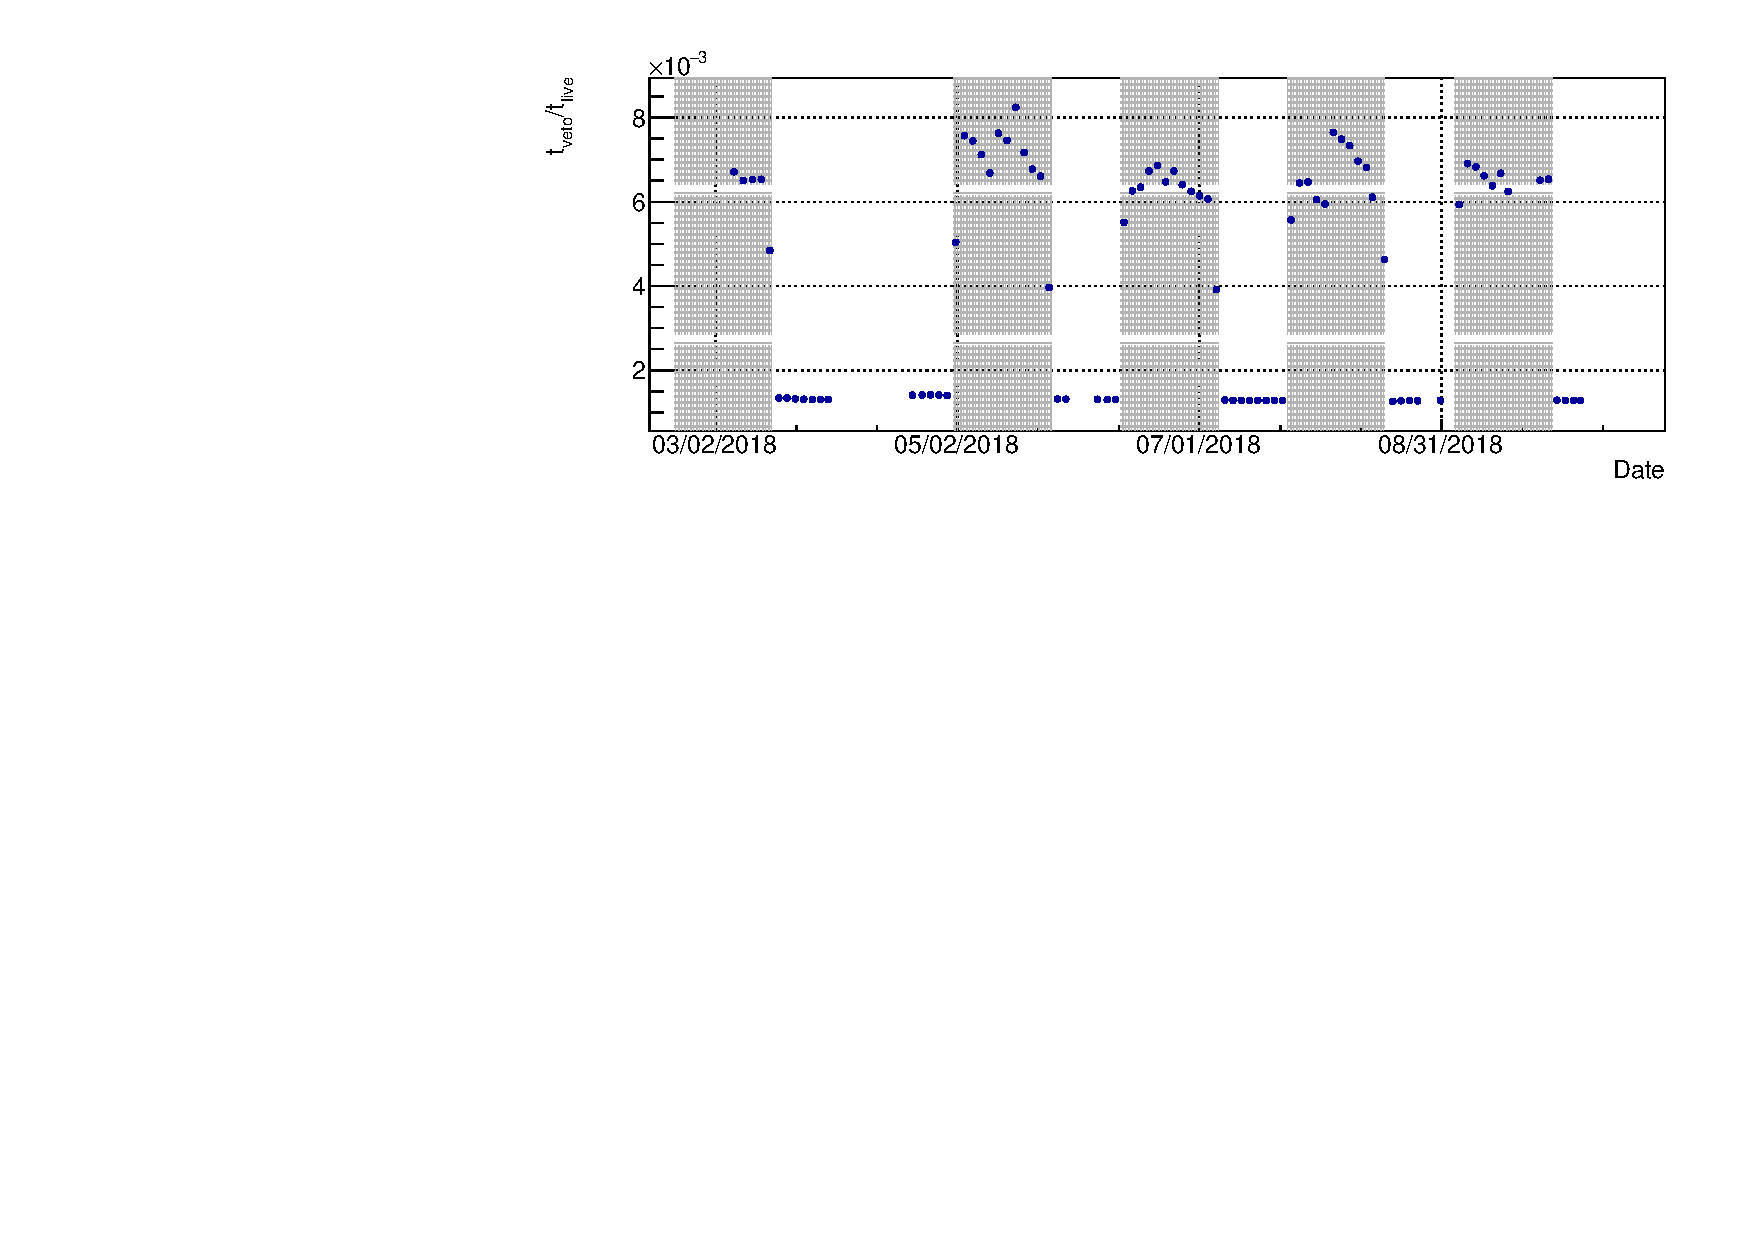
\includegraphics[width=0.8\linewidth]{tex/6-ac227-images/AD_RateCalc/VetoTimeVsTime}
	\caption{The dead time, as a fraction of livetime, due to the pileup veto versus time. Shaded areas are reactor on periods.}
	\label{fig:vetotimevstime}
\end{figure}



The efficiency is calculated for energy and PSD cuts on both prompt and delay events, and for the $\Delta z$ cut.
This is done by fitting each distribution with a Gaussian $\pm 2\sigma$ from the mean, with the exception of the prompt energy which is fit from -1.3$\sigma$ to +0.6$\sigma$.
The efficiency is then calculated as the ratio of the integral of the Gaussian
between the cuts for that distribution to the integral between $\pm \infty$, as defined in Equation~\ref{eq:Eff}.
The error on the efficiency is treated as a binomial error.
For an example of the distributions and fits for a typical segment see Figure~\ref{fig:RnPoDist}.

\begin{align}
	\text{Eff} = \frac{\int_{\text{low-cut}}^{\text{high-cut}}g(u) du}{\int_{-\infty}^{\infty}g(u) du}
	&& \sigma_{\text{Eff}} =\sqrt{\frac{\text{Eff}(1-\text{Eff})}{N}}
	\label{eq:Eff}
\end{align}	

It should be noted here that although the \Rn energy distribution has a high energy tail, due to the accompanying gammas, the efficiency is calculated using a single Gaussian fit around the peak.
This is valid as long as the high energy cut is always wide enough to include the whole high energy tail, which is true for this analysis.

In general the total efficiency is 99.9\% or higher, for RnPo rates calculated in individual segments or versus time.
Figures~\ref{fig:efficiencypercell} and \ref{fig:efficiencyvstime} show the efficiency calculated for all distributions for all individual segments and versus time, respectively.

\begin{figure}[H]
	\begin{subfigure}{0.5\linewidth}
	\centering
	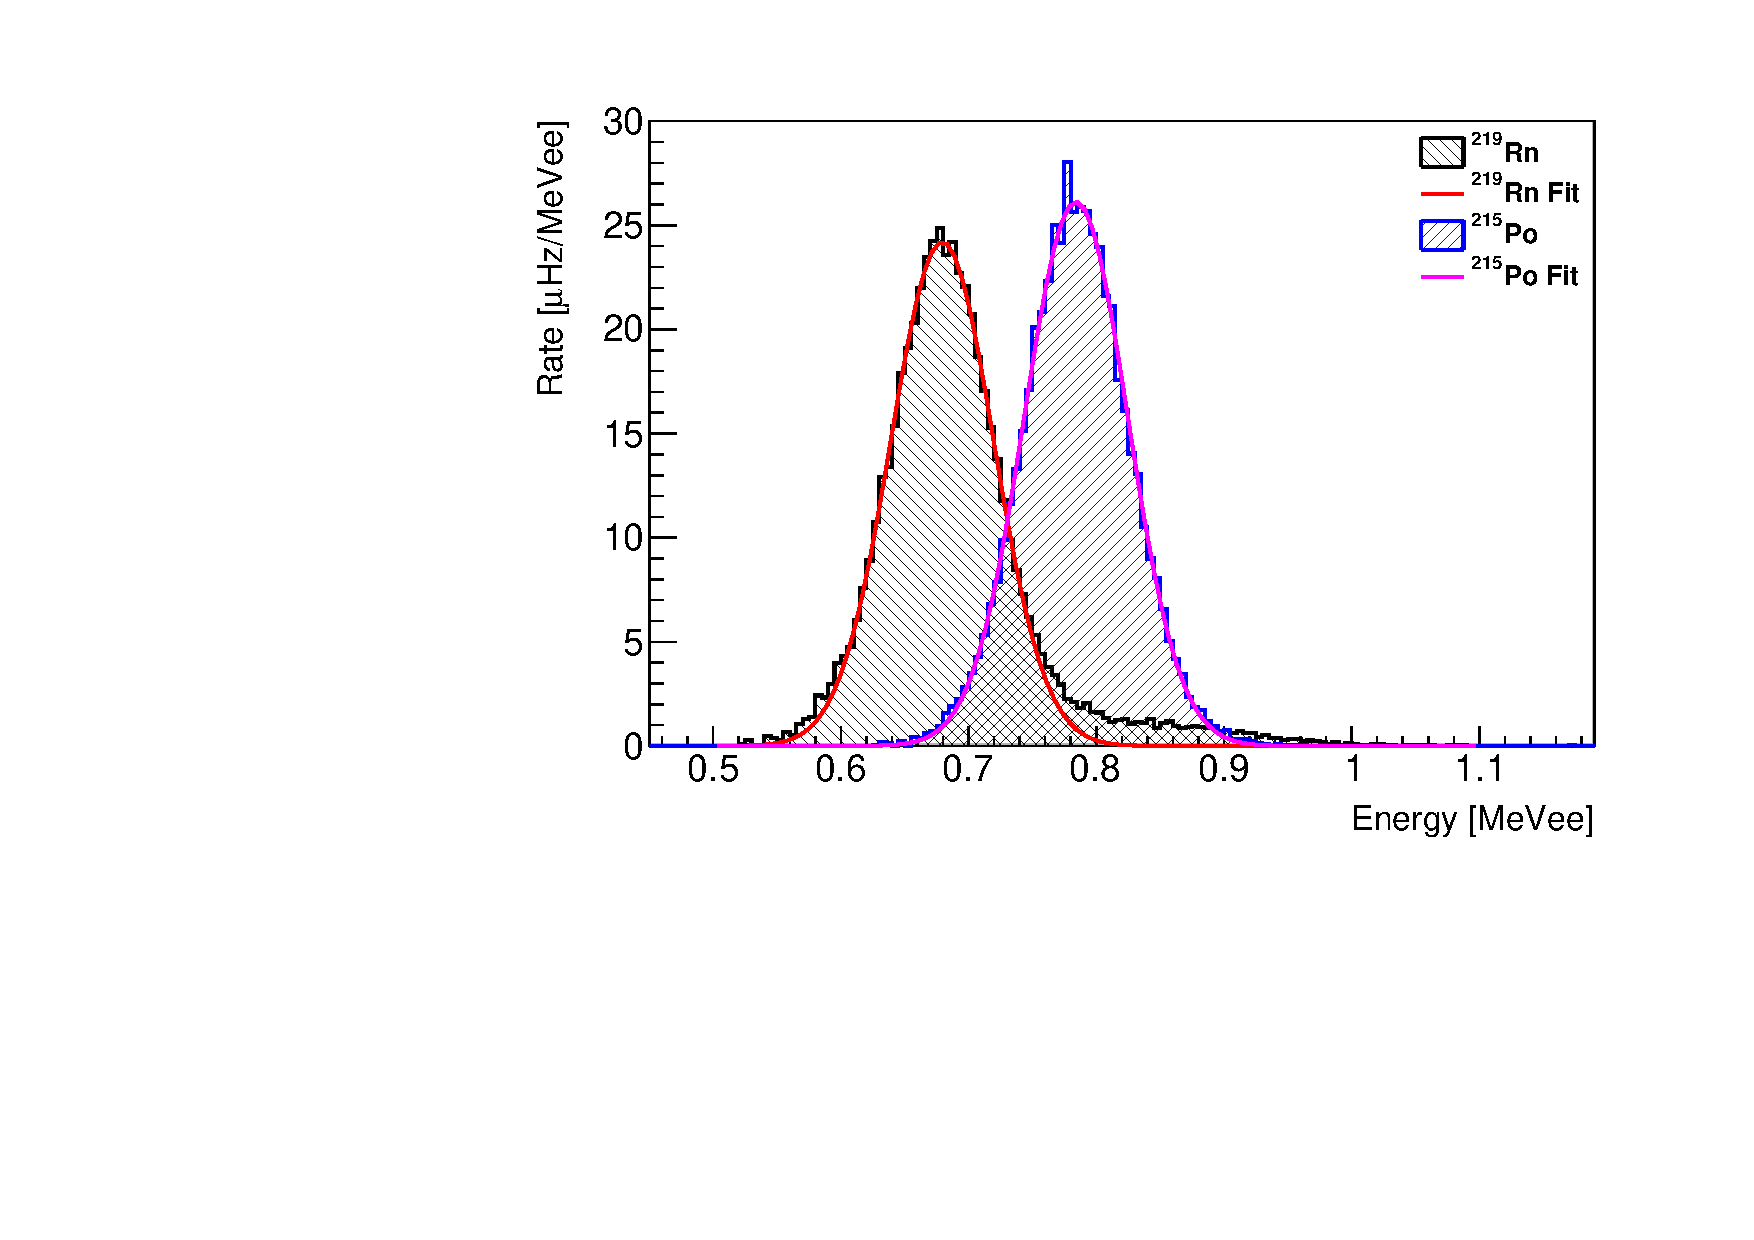
\includegraphics[width=0.95\linewidth]{tex/6-ac227-images/AD_RateCalc/RnPoEn_Seg76}
	\caption{}
	\label{fig:rnpoenseg76}
\end{subfigure}%
\begin{subfigure}{0.5\linewidth}
	\centering
	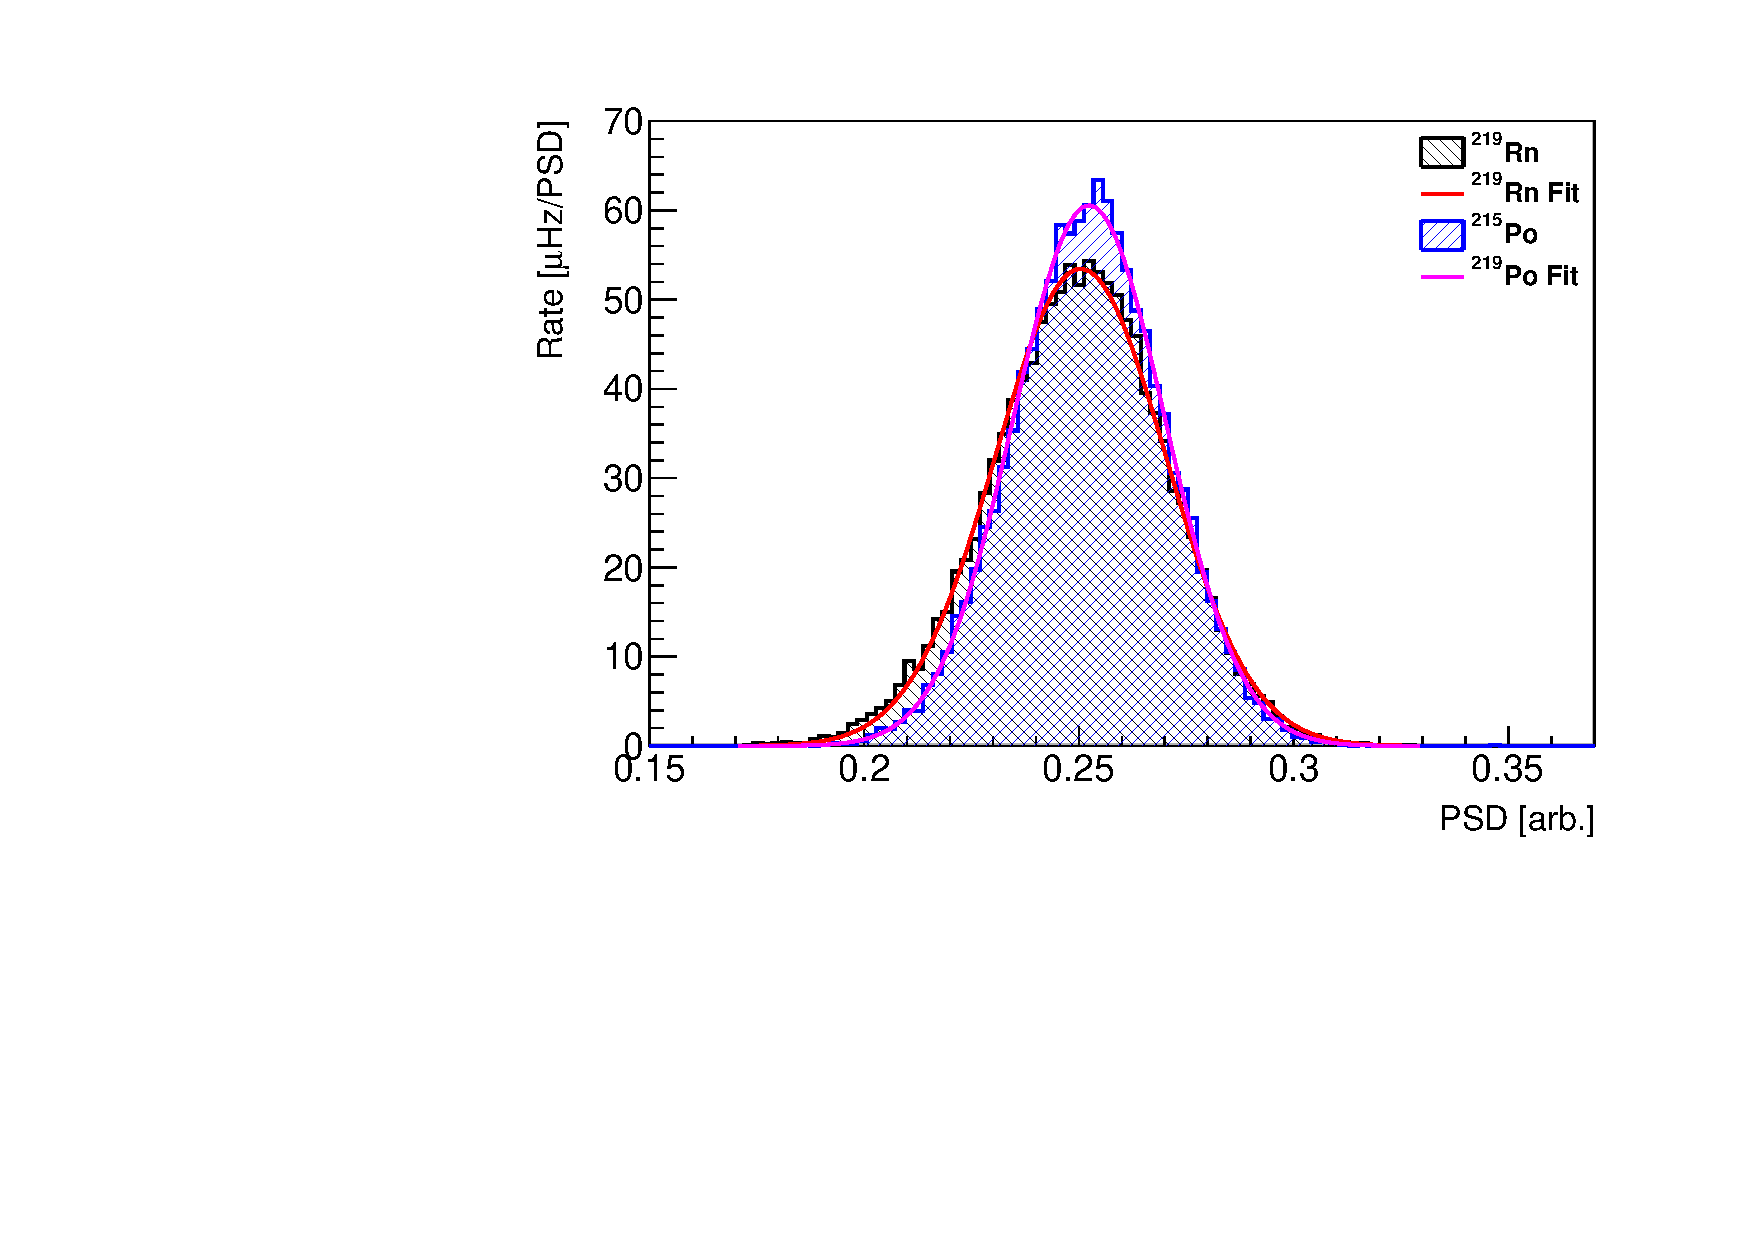
\includegraphics[width=0.95\linewidth]{tex/6-ac227-images/AD_RateCalc/RnPoPSD_Seg76}
	\caption{}
	\label{fig:rnpopsdseg76}
\end{subfigure}
\begin{subfigure}{1\linewidth}
	\centering
	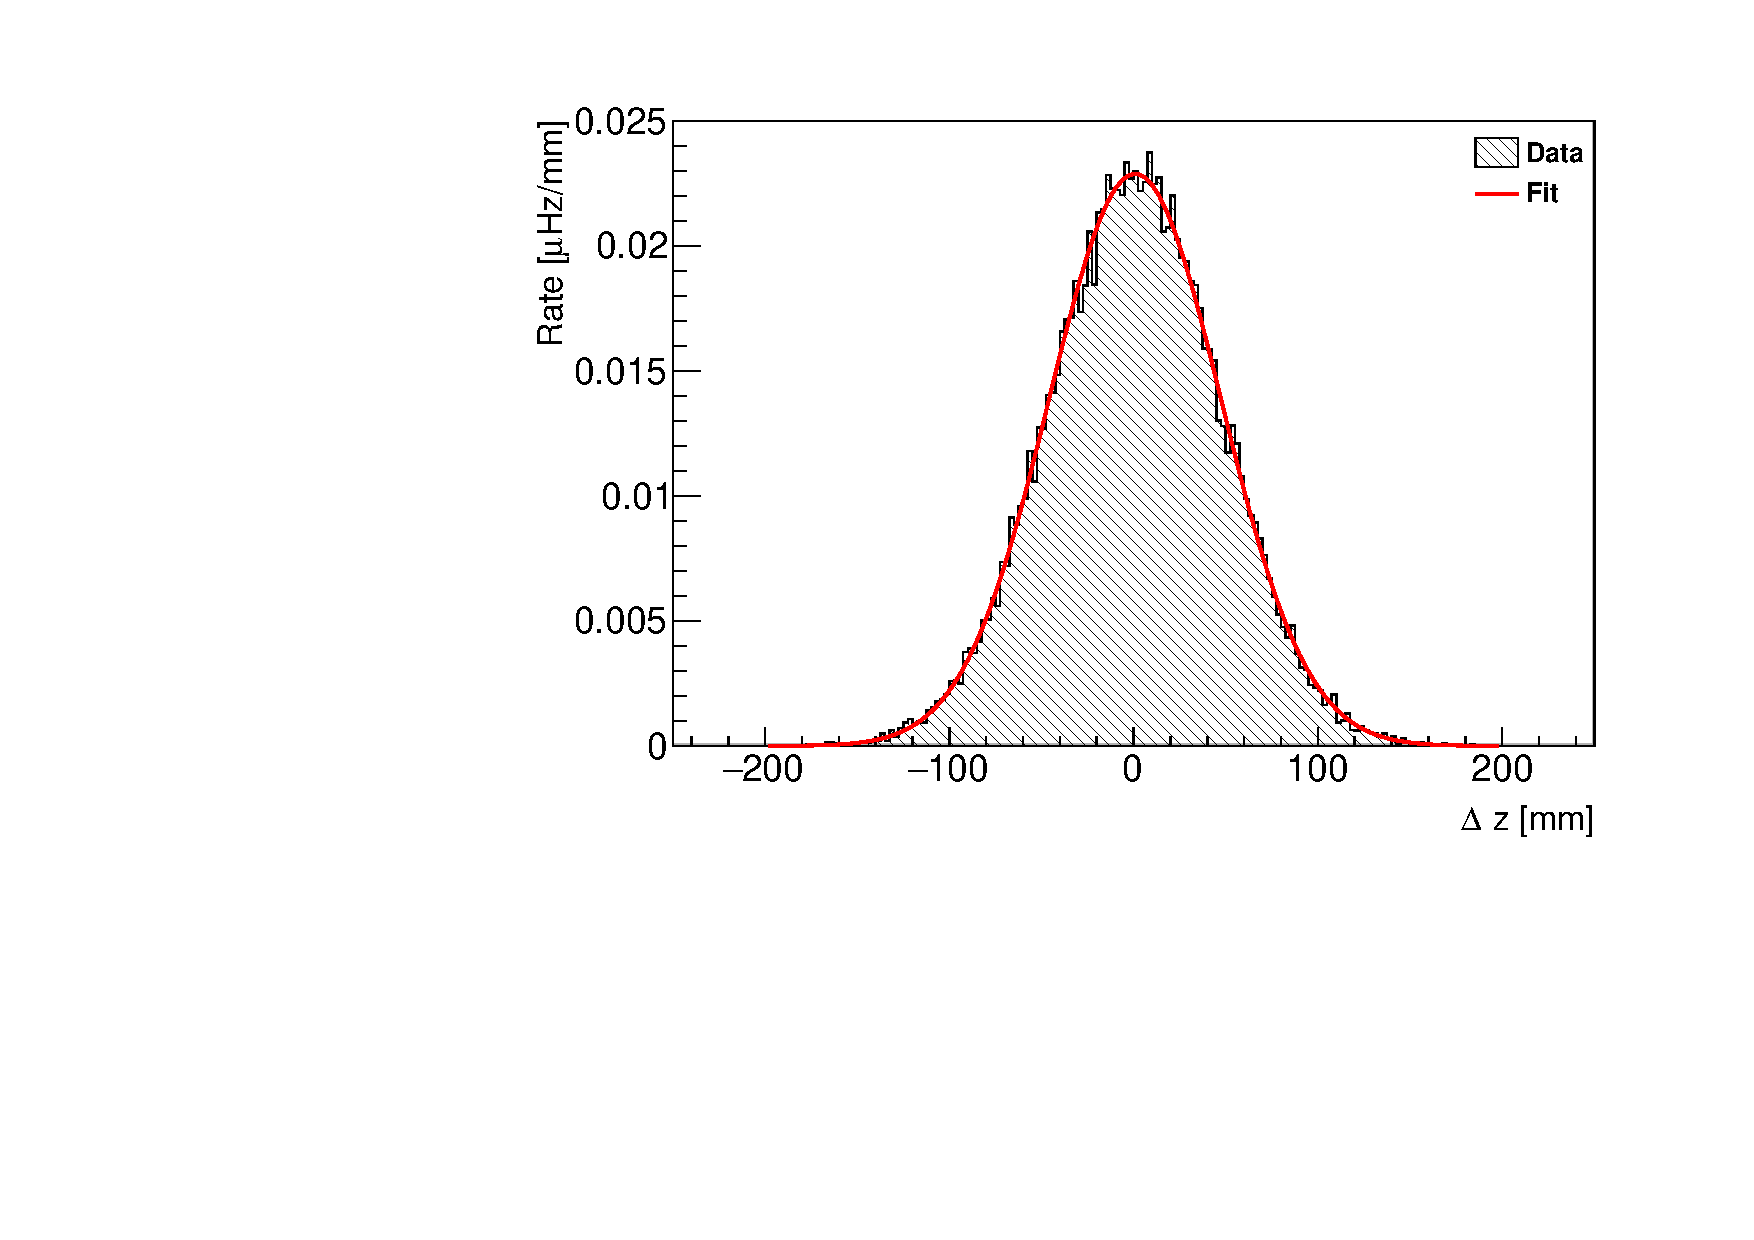
\includegraphics[width=0.475\linewidth]{tex/6-ac227-images/AD_RateCalc/RnPoDz_Seg76}
	\caption{}
	\label{fig:rnpodzseg76}
\end{subfigure}
\caption{Energy (a), PSD (b), and $\Delta z$ (c) distributions for RnPo events in a typical segment integrated over all time. Also shown are the results of fitting each distribution with a Gaussian for the purpose of calculating the cut efficiencies.}
\label{fig:RnPoDist}
\end{figure}


\begin{figure}[h]
	\centering
	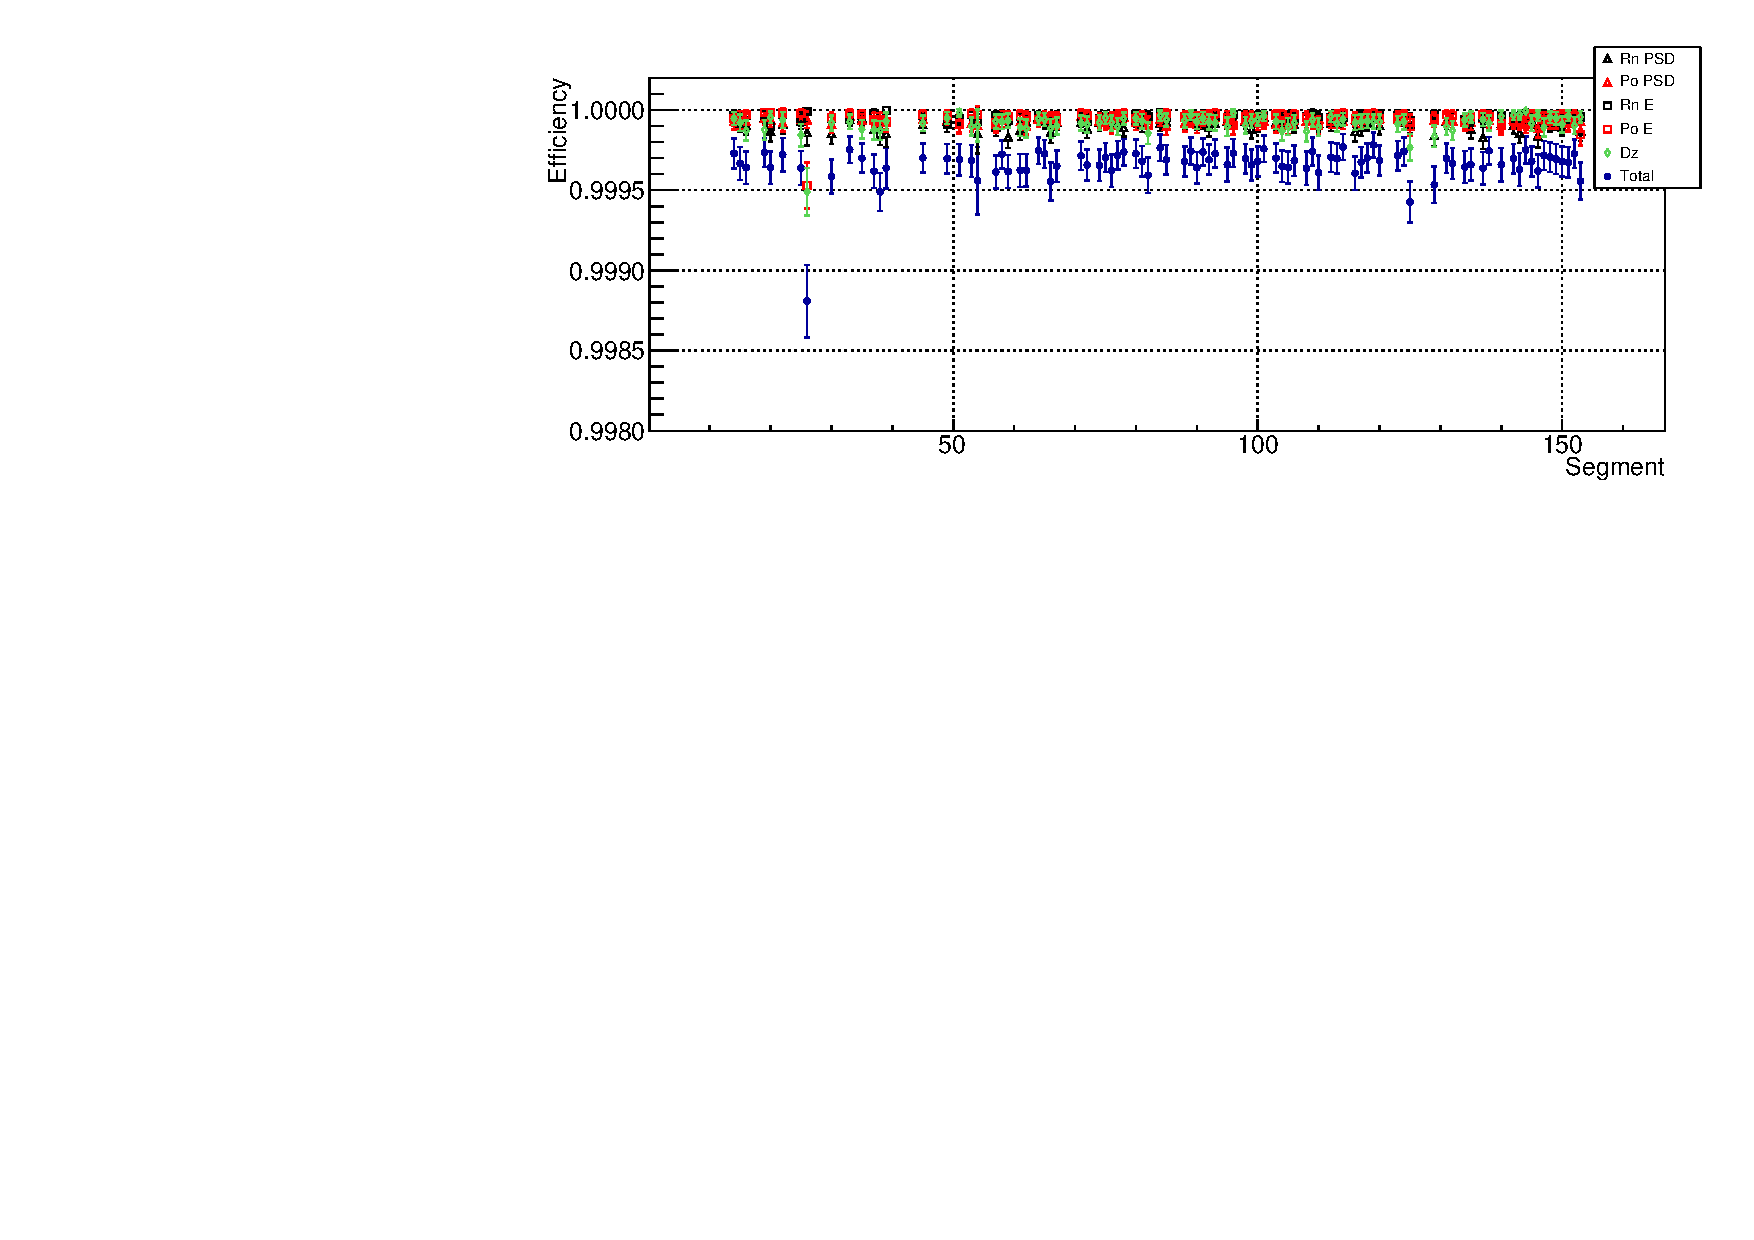
\includegraphics[width=0.9\linewidth]{tex/6-ac227-images/AD_RateCalc/EfficiencyPerCell}
	\caption{Cut efficiencies calculated for RnPo events in individual segments integrated over all time.}
	\label{fig:efficiencypercell}
\end{figure}

\begin{figure}[h]
	\centering
	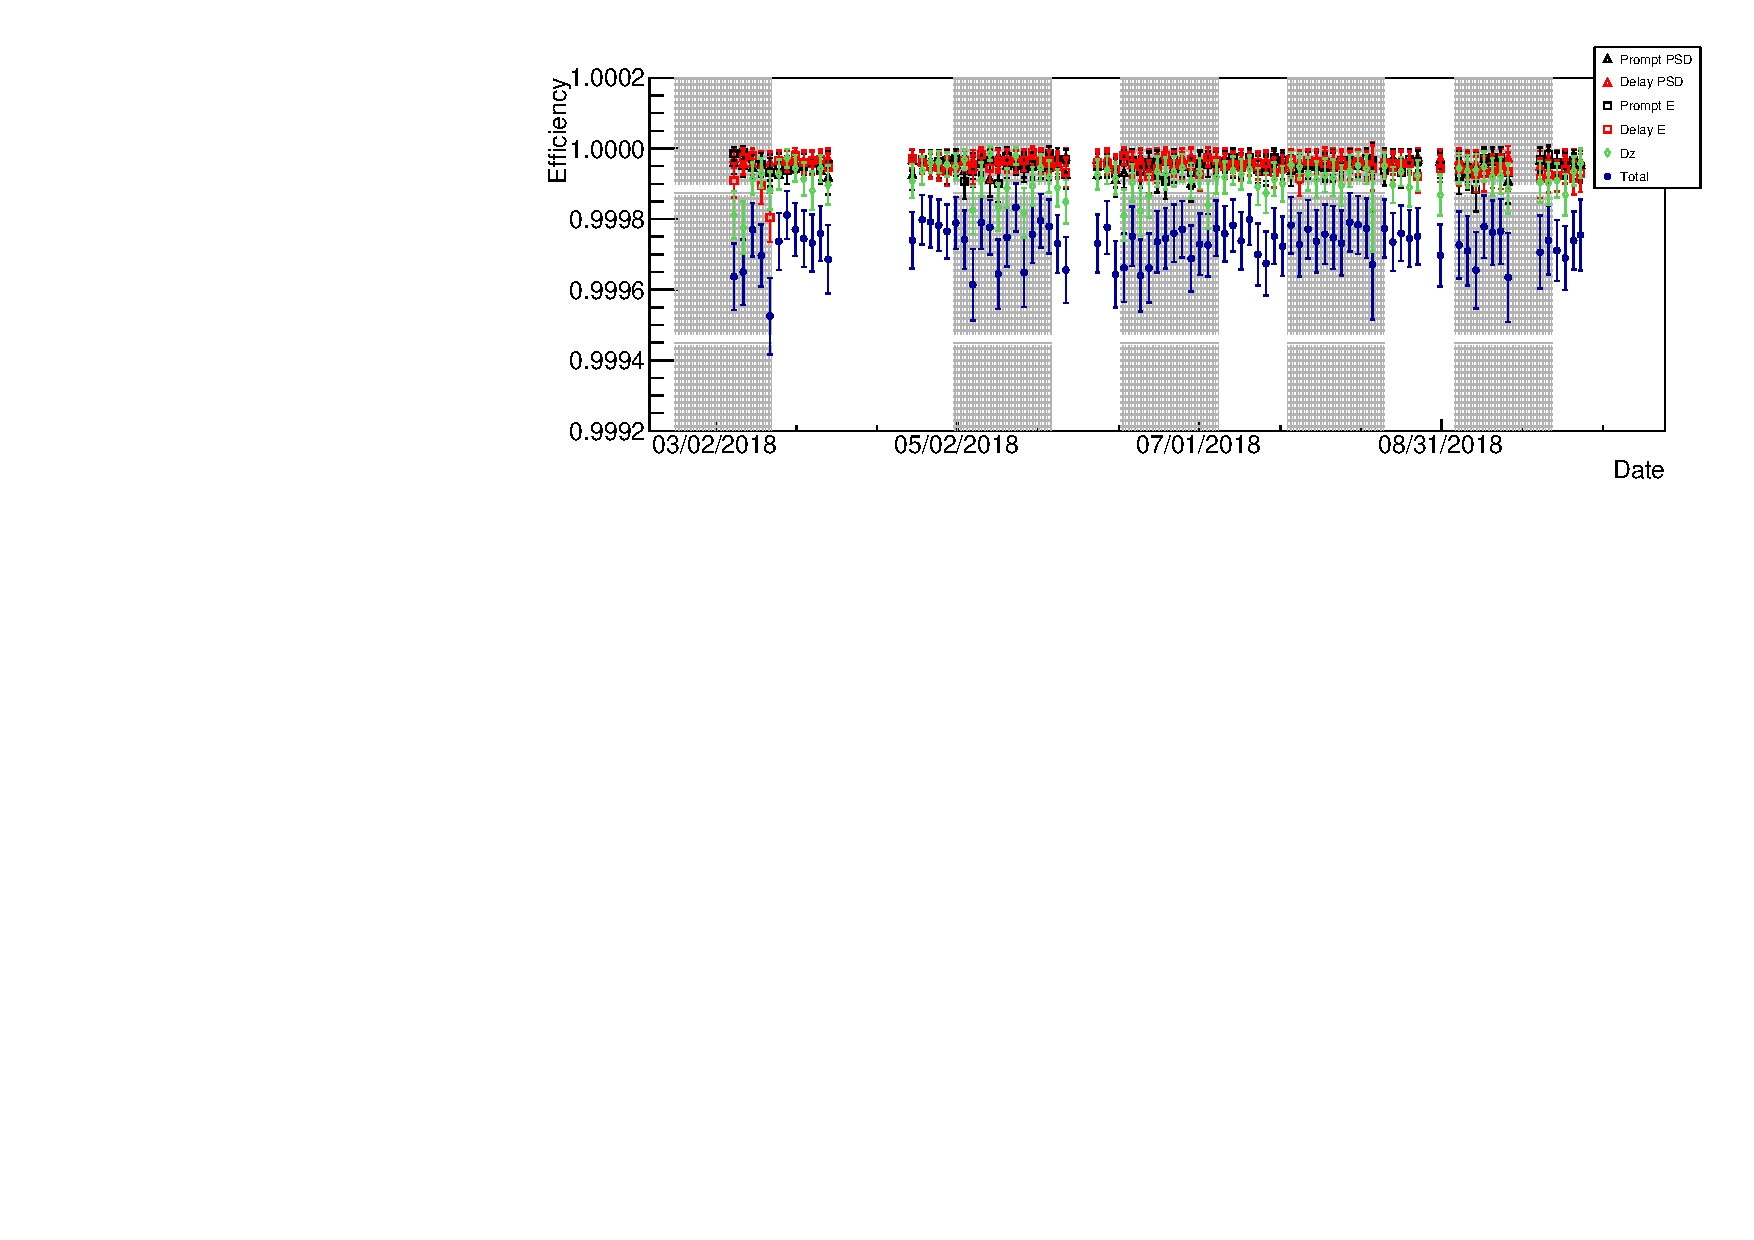
\includegraphics[width=0.9\linewidth]{tex/6-ac227-images/AD_RateCalc/EfficiencyVsTime}
	\caption{Cut efficiencies calculated for RnPo events versus time integrated over all segments. Shaded areas are reactor on periods.}
	\label{fig:efficiencyvstime}
\end{figure}


\subsection{Detector Performance as Tracked with \Ac}

Though \Ac was added to the detector to track the product of efficiency$\times$volume for all segments, the mono-energetic \Po $\alpha$ is also useful for tracking the performance of the detector and the applied calibrations.


\begin{figure}[h]
	\centering
	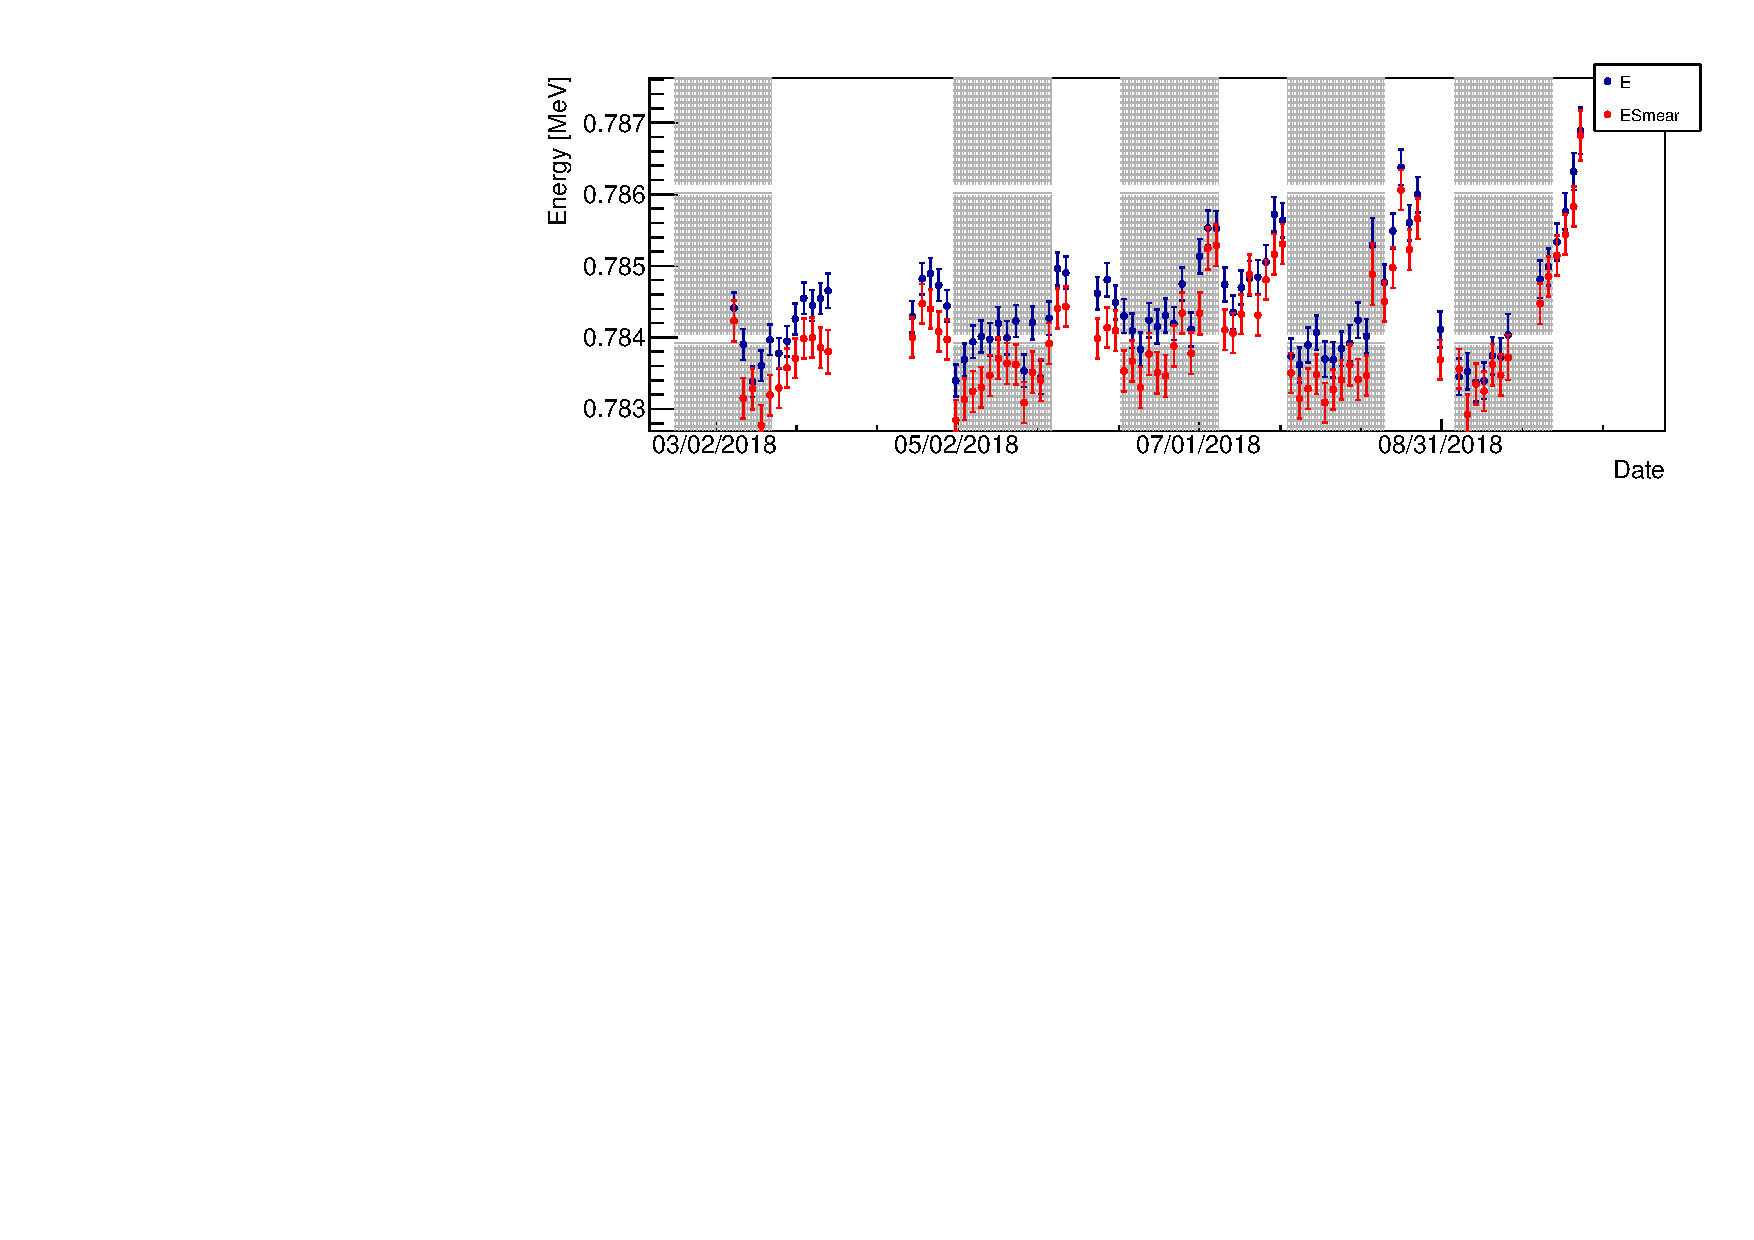
\includegraphics[width=0.9\linewidth]{tex/6-ac227-images/DetPerformance/PoEnMeanVsTime}
	\caption{}
	\label{fig:poenmeanvstime}
\end{figure}

\begin{figure}[h]
	\centering
	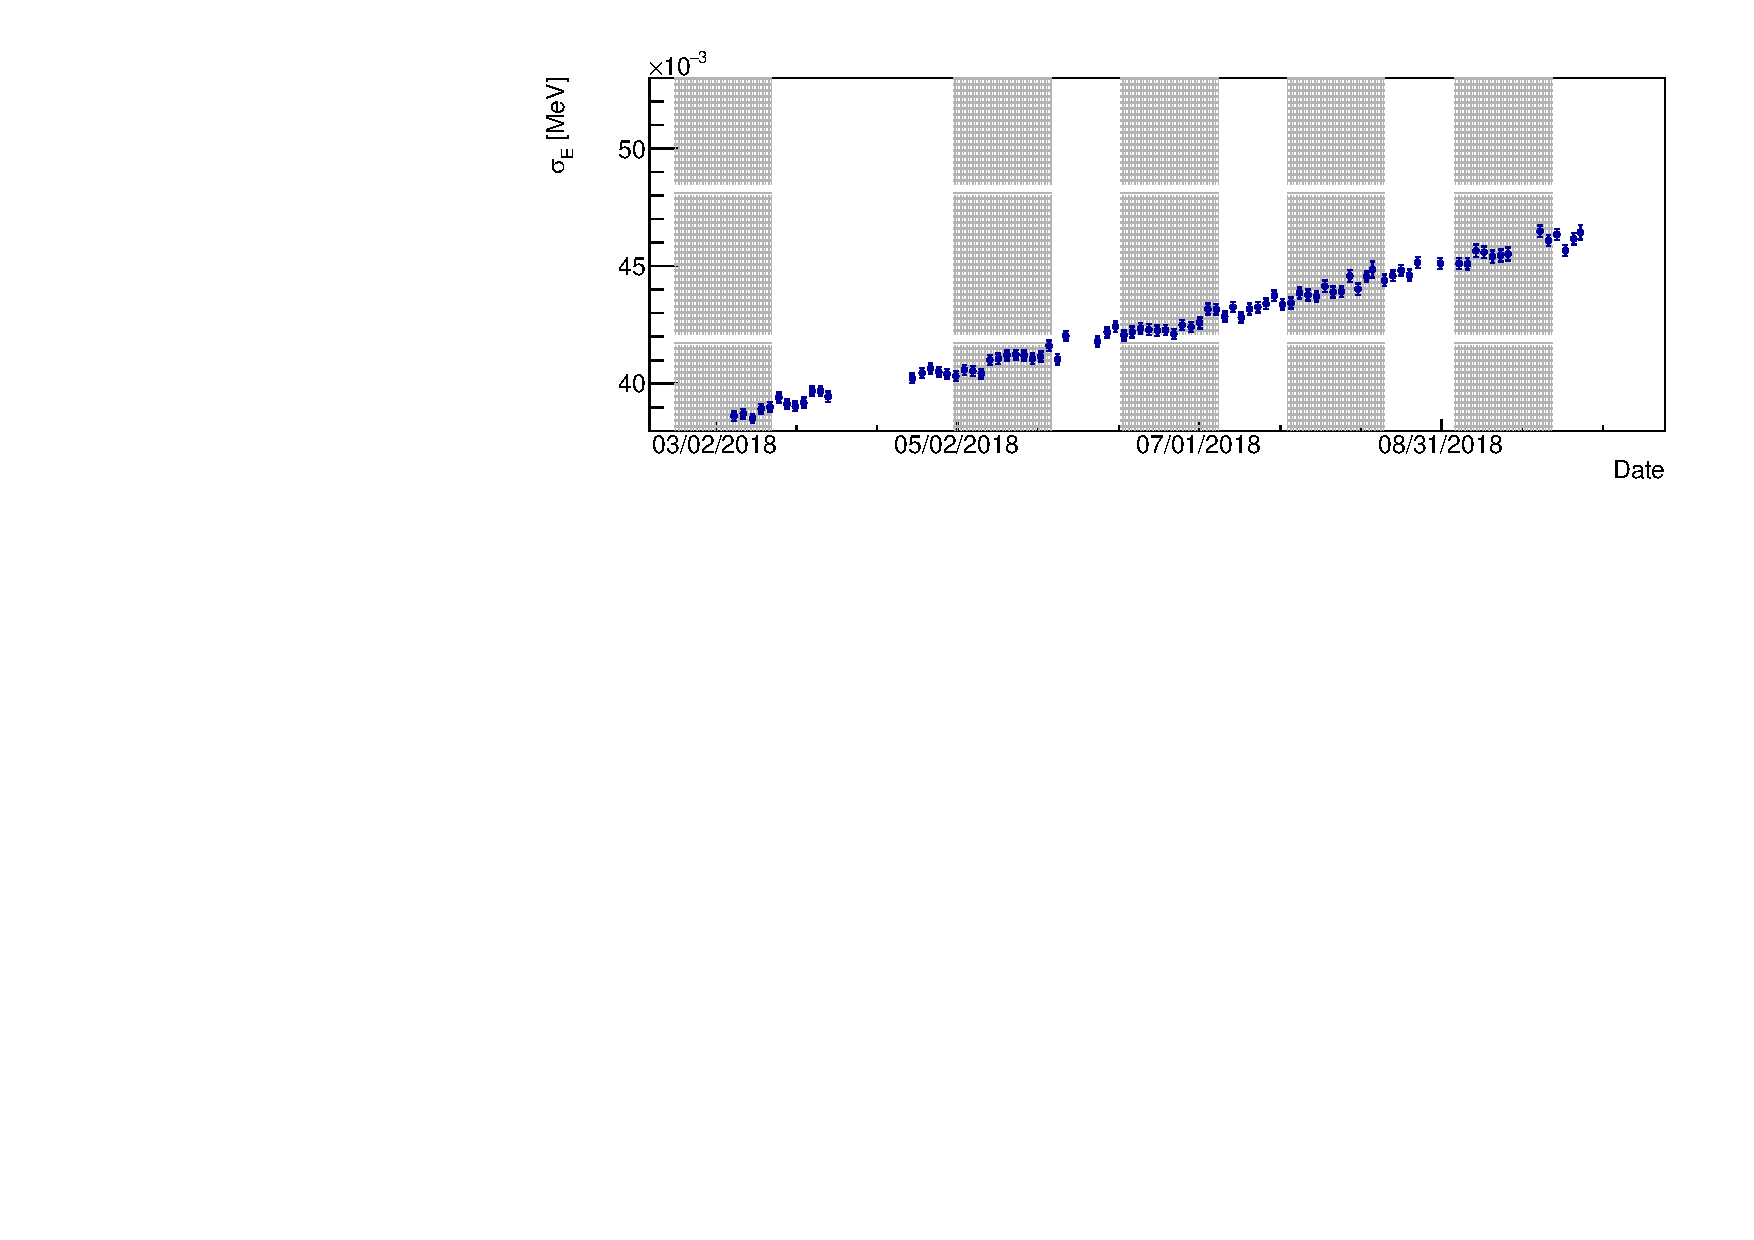
\includegraphics[width=0.9\linewidth]{tex/6-ac227-images/DetPerformance/PoEnSigmaVsTime}
	\caption{}
	\label{fig:poensigmavstime}
\end{figure}


\begin{figure}[h]
	\centering
	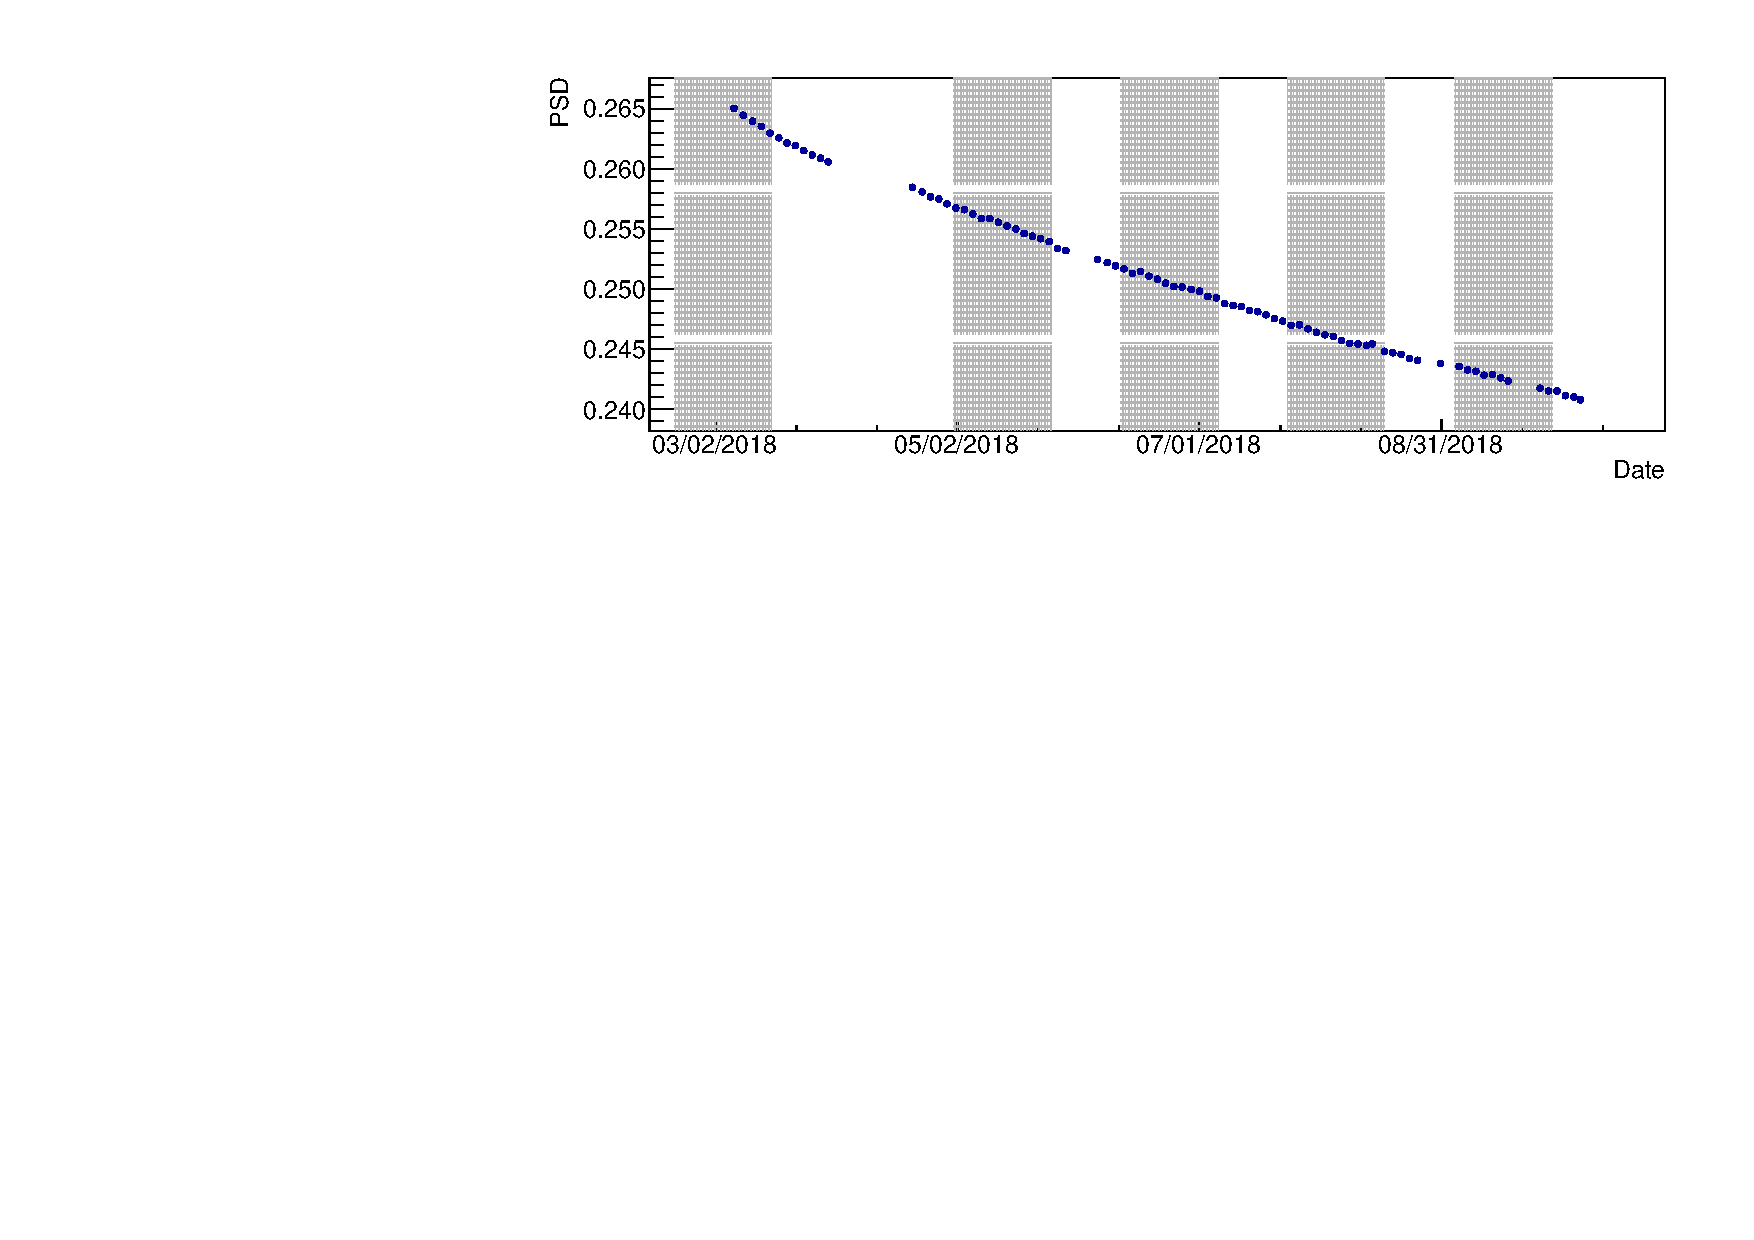
\includegraphics[width=0.9\linewidth]{tex/6-ac227-images/DetPerformance/PoPSDMeanVsTime}
	\caption{}
	\label{fig:popsdmeanvstime}
\end{figure}


\begin{figure}[h]
	\centering
	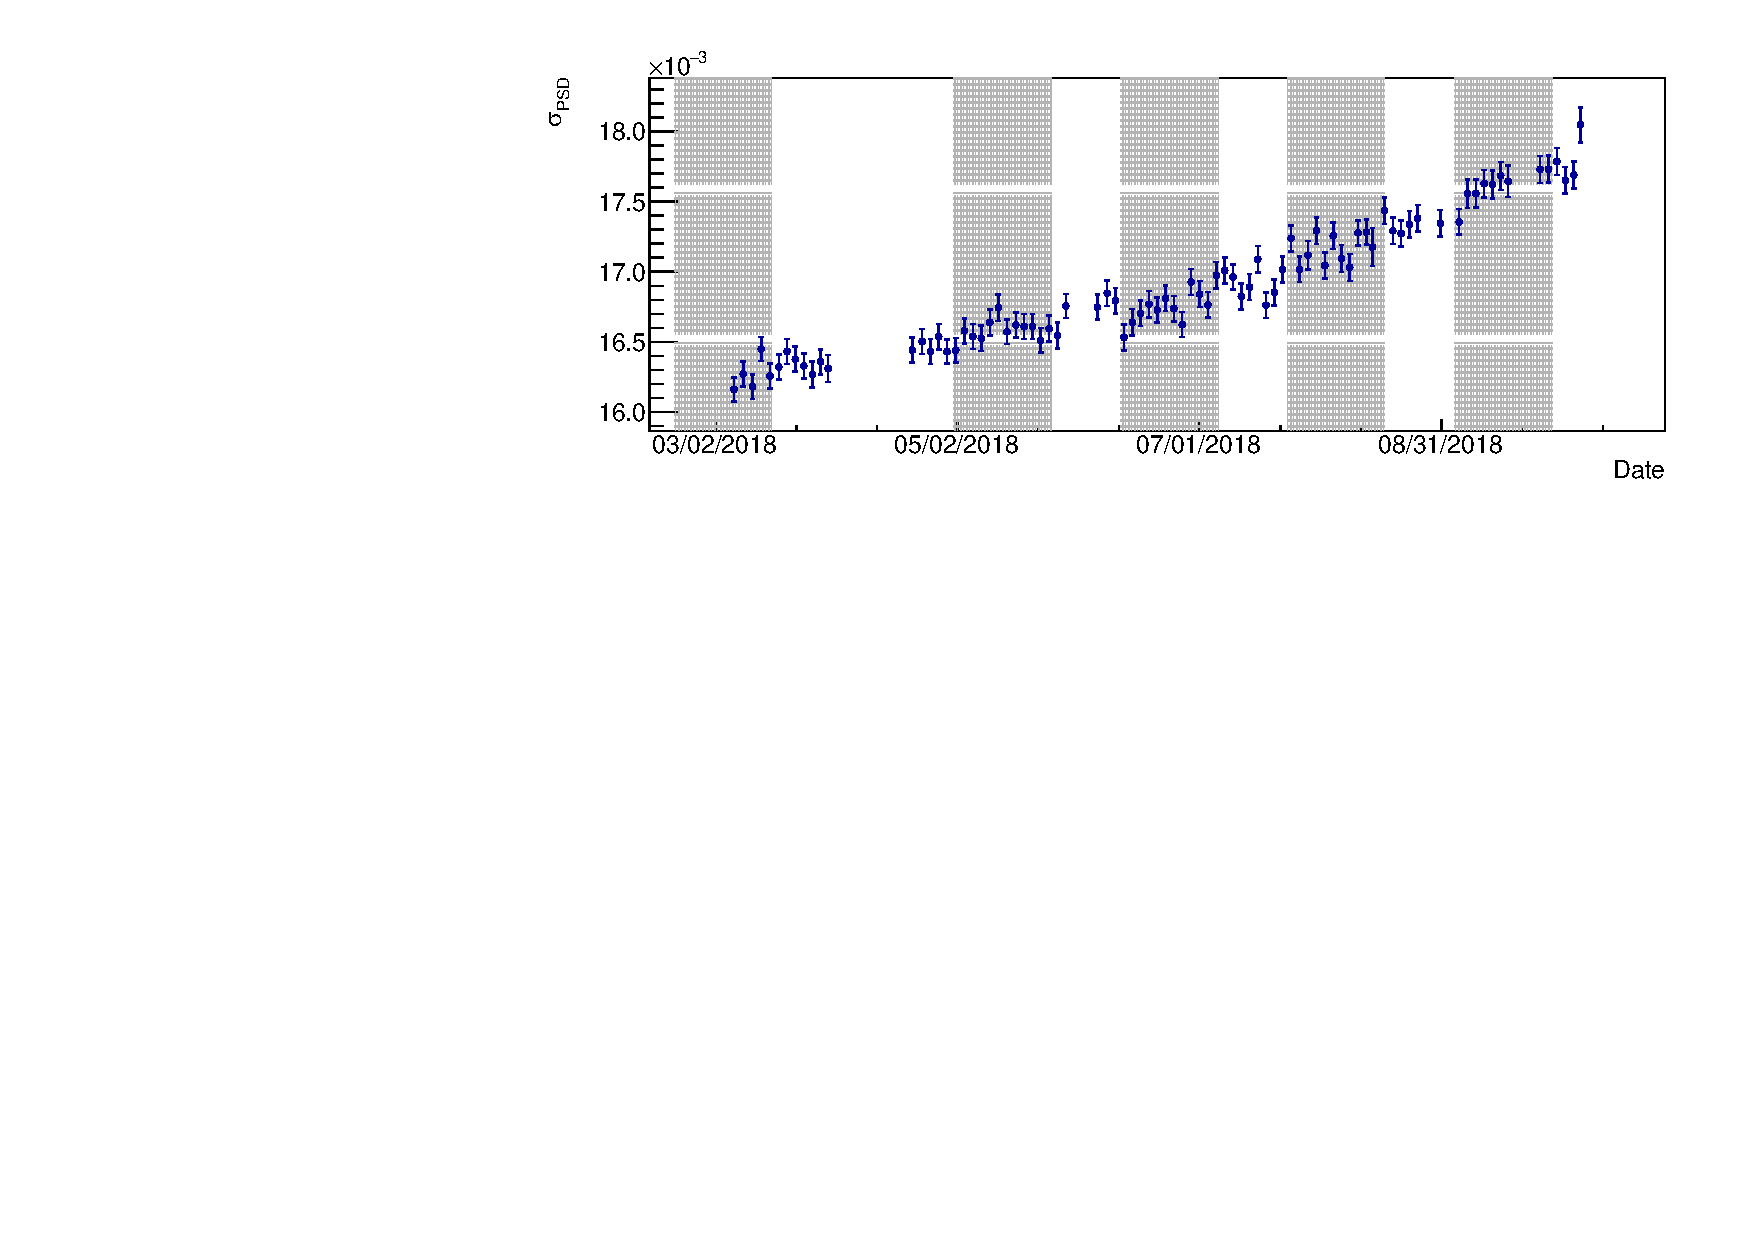
\includegraphics[width=0.9\linewidth]{tex/6-ac227-images/DetPerformance/PoPSDSigmaVsTime}
	\caption{}
	\label{fig:popsdsigmavstime}
\end{figure}


\begin{figure}[h]
	\centering
	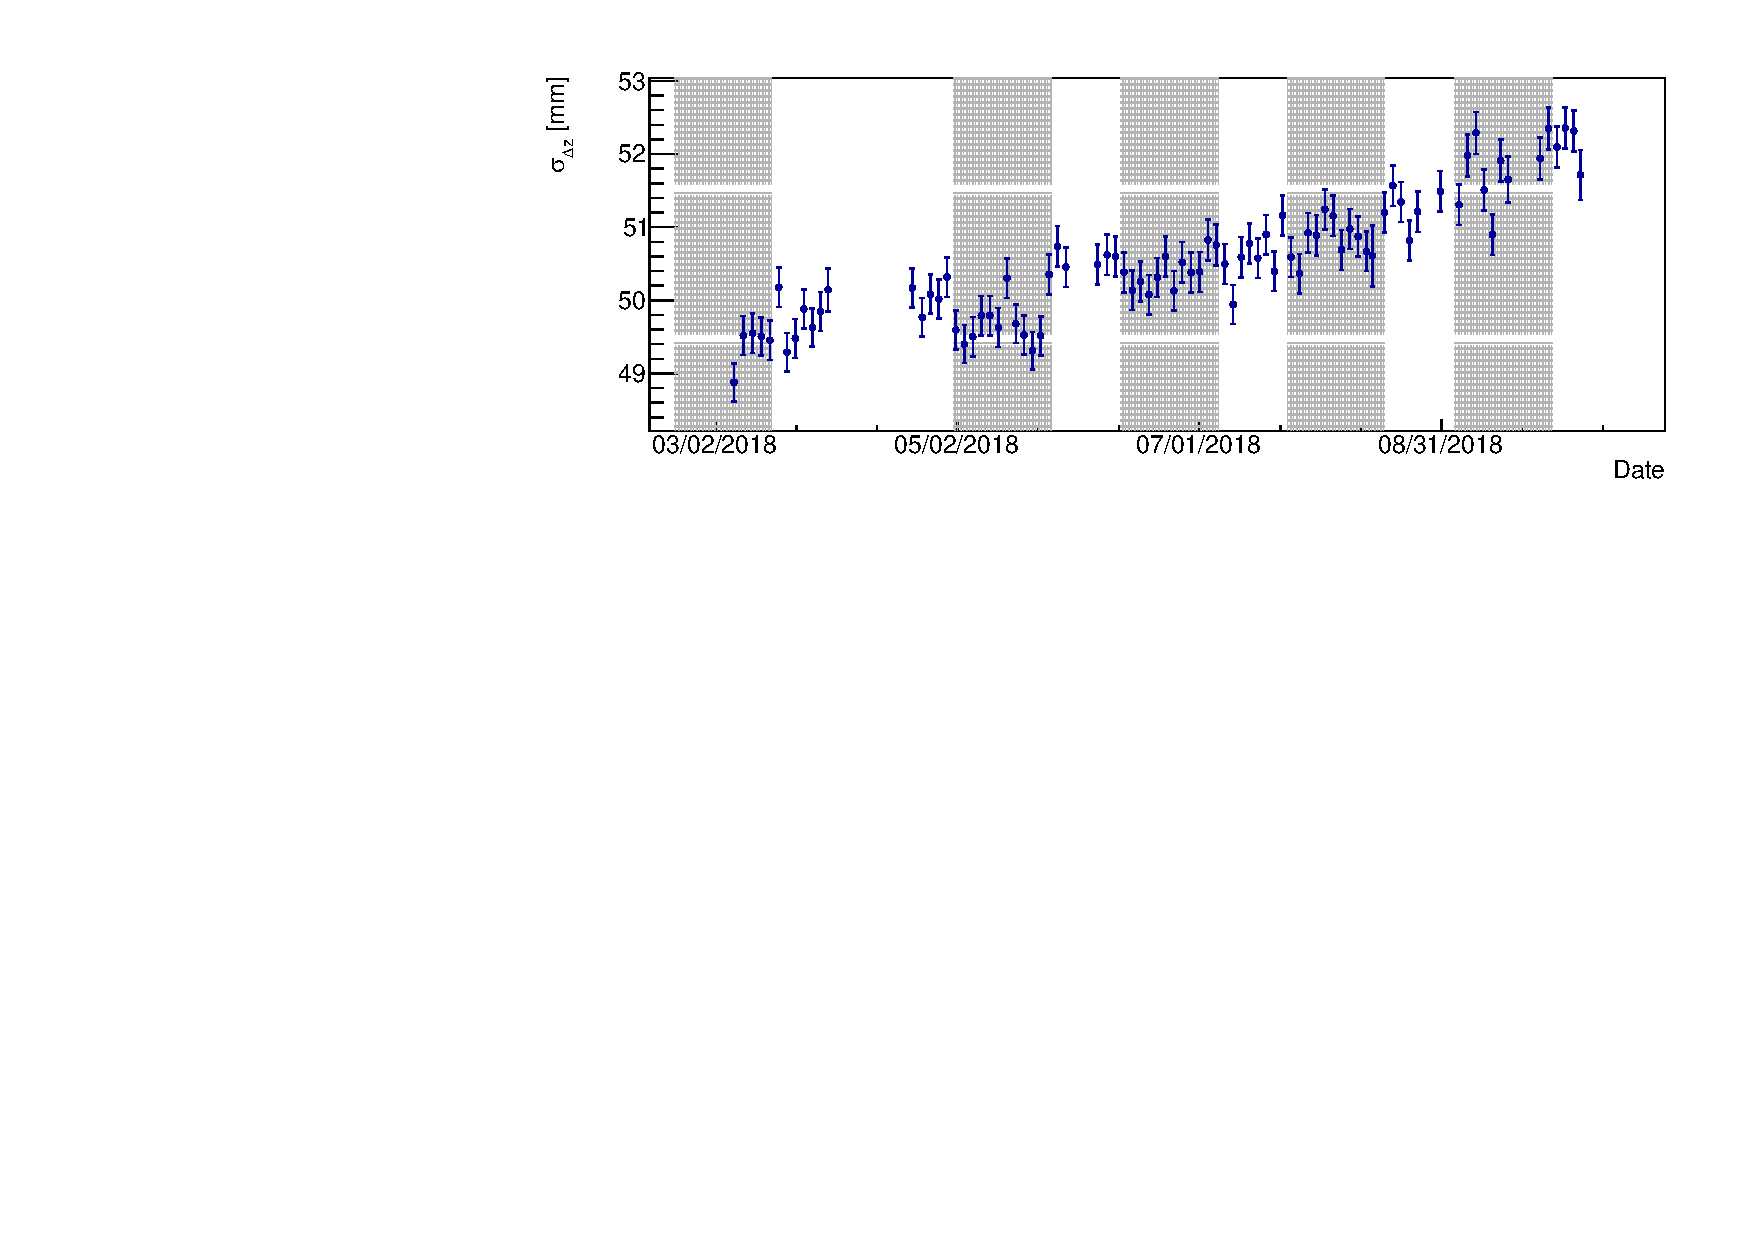
\includegraphics[width=0.9\linewidth]{tex/6-ac227-images/DetPerformance/RnPoDzSigmaVsTime}
	\caption{}
	\label{fig:rnpodzsigmavstime}
\end{figure}

\todo{INCLUDE SEGMENT PLOT}



\subsection{\Ac Rate versus Time}

\subsection{\Ac Rate in Individual Segments}


\subsection{Systematic Errors}

\subsubsection{Energy, PSD, and $\Delta$z Cuts}
\subsubsection{Other Coincident Alphas}
